\documentclass{article}


% if you need to pass options to natbib, use, e.g.:
\PassOptionsToPackage{numbers, sort, compress}{natbib}
%\usepackage[numbers,sort&compress]{natbib}
% before loading neurips_2023


% ready for submission
% \usepackage{neurips_2023}


% to compile a preprint version, e.g., for submission to arXiv, add add the
% [preprint] option:
% \usepackage[preprint]{neurips_2023}


% to compile a camera-ready version, add the [final] option, e.g.:
\usepackage[final]{neurips_2023}


% to avoid loading the natbib package, add option nonatbib:
%    \usepackage[nonatbib]{neurips_2023}


\usepackage[utf8]{inputenc} % allow utf-8 input
\usepackage[T1]{fontenc}    % use 8-bit T1 fonts
\usepackage[colorlinks=true, citecolor=blue, linkcolor=black, urlcolor=Violet]{hyperref}       % hyperlinks
%\usepackage{hyperref}
\usepackage{url}            % simple URL typesetting
\usepackage{booktabs}       % professional-quality tables
\usepackage{amsfonts}       % blackboard math symbols
\usepackage{nicefrac}       % compact symbols for 1/2, etc.
\usepackage{microtype}      % microtypography
\usepackage[dvipsnames]{xcolor}         % colors
\usepackage{subfigure}
\usepackage{multirow}
\usepackage{multicol} 
\usepackage{pifont}
\usepackage{graphicx}
\usepackage{algorithm}
\usepackage{algorithmic}
\usepackage{caption}
\usepackage{amsmath}
\usepackage{amssymb}
\usepackage[font={footnotesize}]{caption}


\usepackage[utf8]{inputenc} % allow utf-8 input
\usepackage[T1]{fontenc}    % use 8-bit T1 fonts
\usepackage{hyperref}       % hyperlinks
\usepackage{url}            % simple URL typesetting
\usepackage{booktabs}       % professional-quality tables
\usepackage{amsfonts}       % blackboard math symbols
\usepackage{nicefrac}       % compact symbols for 1/2, etc.
\usepackage{microtype}      % microtypography
%\usepackage{xcolor}         % colors
% \usepackage[table]{xcolor}
% \usepackage{tcolorbox}

 
 \usepackage{graphicx}
\usepackage{subfigure} 
\usepackage{pifont}
%%%%%%%%%%%%%%%% Customized by SL
% %%%%% NEW MATH DEFINITIONS %%%%%

\usepackage{amsmath,amsfonts,bm}

% Mark sections of captions for referring to divisions of figures
\newcommand{\figleft}{{\em (Left)}}
\newcommand{\figcenter}{{\em (Center)}}
\newcommand{\figright}{{\em (Right)}}
\newcommand{\figtop}{{\em (Top)}}
\newcommand{\figbottom}{{\em (Bottom)}}
\newcommand{\captiona}{{\em (a)}}
\newcommand{\captionb}{{\em (b)}}
\newcommand{\captionc}{{\em (c)}}
\newcommand{\captiond}{{\em (d)}}

% Highlight a newly defined term
\newcommand{\newterm}[1]{{\bf #1}}


% Figure reference, lower-case.
\def\figref#1{figure~\ref{#1}}
% Figure reference, capital. For start of sentence
\def\Figref#1{Figure~\ref{#1}}
\def\twofigref#1#2{figures \ref{#1} and \ref{#2}}
\def\quadfigref#1#2#3#4{figures \ref{#1}, \ref{#2}, \ref{#3} and \ref{#4}}
% Section reference, lower-case.
\def\secref#1{section~\ref{#1}}
% Section reference, capital.
\def\Secref#1{Section~\ref{#1}}
% Reference to two sections.
\def\twosecrefs#1#2{sections \ref{#1} and \ref{#2}}
% Reference to three sections.
\def\secrefs#1#2#3{sections \ref{#1}, \ref{#2} and \ref{#3}}
% Reference to an equation, lower-case.
\def\eqref#1{equation~\ref{#1}}
% Reference to an equation, upper case
\def\Eqref#1{Equation~\ref{#1}}
% A raw reference to an equation---avoid using if possible
\def\plaineqref#1{\ref{#1}}
% Reference to a chapter, lower-case.
\def\chapref#1{chapter~\ref{#1}}
% Reference to an equation, upper case.
\def\Chapref#1{Chapter~\ref{#1}}
% Reference to a range of chapters
\def\rangechapref#1#2{chapters\ref{#1}--\ref{#2}}
% Reference to an algorithm, lower-case.
\def\algref#1{algorithm~\ref{#1}}
% Reference to an algorithm, upper case.
\def\Algref#1{Algorithm~\ref{#1}}
\def\twoalgref#1#2{algorithms \ref{#1} and \ref{#2}}
\def\Twoalgref#1#2{Algorithms \ref{#1} and \ref{#2}}
% Reference to a part, lower case
\def\partref#1{part~\ref{#1}}
% Reference to a part, upper case
\def\Partref#1{Part~\ref{#1}}
\def\twopartref#1#2{parts \ref{#1} and \ref{#2}}

\def\ceil#1{\lceil #1 \rceil}
\def\floor#1{\lfloor #1 \rfloor}
\def\1{\bm{1}}
\newcommand{\train}{\mathcal{D}}
\newcommand{\valid}{\mathcal{D_{\mathrm{valid}}}}
\newcommand{\test}{\mathcal{D_{\mathrm{test}}}}

\def\eps{{\epsilon}}


% Random variables
\def\reta{{\textnormal{$\eta$}}}
\def\ra{{\textnormal{a}}}
\def\rb{{\textnormal{b}}}
\def\rc{{\textnormal{c}}}
\def\rd{{\textnormal{d}}}
\def\re{{\textnormal{e}}}
\def\rf{{\textnormal{f}}}
\def\rg{{\textnormal{g}}}
\def\rh{{\textnormal{h}}}
\def\ri{{\textnormal{i}}}
\def\rj{{\textnormal{j}}}
\def\rk{{\textnormal{k}}}
\def\rl{{\textnormal{l}}}
% rm is already a command, just don't name any random variables m
\def\rn{{\textnormal{n}}}
\def\ro{{\textnormal{o}}}
\def\rp{{\textnormal{p}}}
\def\rq{{\textnormal{q}}}
\def\rr{{\textnormal{r}}}
\def\rs{{\textnormal{s}}}
\def\rt{{\textnormal{t}}}
\def\ru{{\textnormal{u}}}
\def\rv{{\textnormal{v}}}
\def\rw{{\textnormal{w}}}
\def\rx{{\textnormal{x}}}
\def\ry{{\textnormal{y}}}
\def\rz{{\textnormal{z}}}

% Random vectors
\def\rvepsilon{{\mathbf{\epsilon}}}
\def\rvtheta{{\mathbf{\theta}}}
\def\rva{{\mathbf{a}}}
\def\rvb{{\mathbf{b}}}
\def\rvc{{\mathbf{c}}}
\def\rvd{{\mathbf{d}}}
\def\rve{{\mathbf{e}}}
\def\rvf{{\mathbf{f}}}
\def\rvg{{\mathbf{g}}}
\def\rvh{{\mathbf{h}}}
\def\rvu{{\mathbf{i}}}
\def\rvj{{\mathbf{j}}}
\def\rvk{{\mathbf{k}}}
\def\rvl{{\mathbf{l}}}
\def\rvm{{\mathbf{m}}}
\def\rvn{{\mathbf{n}}}
\def\rvo{{\mathbf{o}}}
\def\rvp{{\mathbf{p}}}
\def\rvq{{\mathbf{q}}}
\def\rvr{{\mathbf{r}}}
\def\rvs{{\mathbf{s}}}
\def\rvt{{\mathbf{t}}}
\def\rvu{{\mathbf{u}}}
\def\rvv{{\mathbf{v}}}
\def\rvw{{\mathbf{w}}}
\def\rvx{{\mathbf{x}}}
\def\rvy{{\mathbf{y}}}
\def\rvz{{\mathbf{z}}}

% Elements of random vectors
\def\erva{{\textnormal{a}}}
\def\ervb{{\textnormal{b}}}
\def\ervc{{\textnormal{c}}}
\def\ervd{{\textnormal{d}}}
\def\erve{{\textnormal{e}}}
\def\ervf{{\textnormal{f}}}
\def\ervg{{\textnormal{g}}}
\def\ervh{{\textnormal{h}}}
\def\ervi{{\textnormal{i}}}
\def\ervj{{\textnormal{j}}}
\def\ervk{{\textnormal{k}}}
\def\ervl{{\textnormal{l}}}
\def\ervm{{\textnormal{m}}}
\def\ervn{{\textnormal{n}}}
\def\ervo{{\textnormal{o}}}
\def\ervp{{\textnormal{p}}}
\def\ervq{{\textnormal{q}}}
\def\ervr{{\textnormal{r}}}
\def\ervs{{\textnormal{s}}}
\def\ervt{{\textnormal{t}}}
\def\ervu{{\textnormal{u}}}
\def\ervv{{\textnormal{v}}}
\def\ervw{{\textnormal{w}}}
\def\ervx{{\textnormal{x}}}
\def\ervy{{\textnormal{y}}}
\def\ervz{{\textnormal{z}}}

% Random matrices
\def\rmA{{\mathbf{A}}}
\def\rmB{{\mathbf{B}}}
\def\rmC{{\mathbf{C}}}
\def\rmD{{\mathbf{D}}}
\def\rmE{{\mathbf{E}}}
\def\rmF{{\mathbf{F}}}
\def\rmG{{\mathbf{G}}}
\def\rmH{{\mathbf{H}}}
\def\rmI{{\mathbf{I}}}
\def\rmJ{{\mathbf{J}}}
\def\rmK{{\mathbf{K}}}
\def\rmL{{\mathbf{L}}}
\def\rmM{{\mathbf{M}}}
\def\rmN{{\mathbf{N}}}
\def\rmO{{\mathbf{O}}}
\def\rmP{{\mathbf{P}}}
\def\rmQ{{\mathbf{Q}}}
\def\rmR{{\mathbf{R}}}
\def\rmS{{\mathbf{S}}}
\def\rmT{{\mathbf{T}}}
\def\rmU{{\mathbf{U}}}
\def\rmV{{\mathbf{V}}}
\def\rmW{{\mathbf{W}}}
\def\rmX{{\mathbf{X}}}
\def\rmY{{\mathbf{Y}}}
\def\rmZ{{\mathbf{Z}}}

% Elements of random matrices
\def\ermA{{\textnormal{A}}}
\def\ermB{{\textnormal{B}}}
\def\ermC{{\textnormal{C}}}
\def\ermD{{\textnormal{D}}}
\def\ermE{{\textnormal{E}}}
\def\ermF{{\textnormal{F}}}
\def\ermG{{\textnormal{G}}}
\def\ermH{{\textnormal{H}}}
\def\ermI{{\textnormal{I}}}
\def\ermJ{{\textnormal{J}}}
\def\ermK{{\textnormal{K}}}
\def\ermL{{\textnormal{L}}}
\def\ermM{{\textnormal{M}}}
\def\ermN{{\textnormal{N}}}
\def\ermO{{\textnormal{O}}}
\def\ermP{{\textnormal{P}}}
\def\ermQ{{\textnormal{Q}}}
\def\ermR{{\textnormal{R}}}
\def\ermS{{\textnormal{S}}}
\def\ermT{{\textnormal{T}}}
\def\ermU{{\textnormal{U}}}
\def\ermV{{\textnormal{V}}}
\def\ermW{{\textnormal{W}}}
\def\ermX{{\textnormal{X}}}
\def\ermY{{\textnormal{Y}}}
\def\ermZ{{\textnormal{Z}}}

% Vectors
\def\vzero{{\bm{0}}}
\def\vone{{\bm{1}}}
\def\vmu{{\bm{\mu}}}
\def\vtheta{{\bm{\theta}}}
\def\vpsi{{\bm{\psi}}}
\def\vsigma{{\bm{\sigma}}}
\def\vlambda{{\bm{\lambda}}}
\def\vgamma{{\bm{\gamma}}}
\def\vomega{{\bm{\omega}}}
\def\va{{\bm{a}}}
\def\vb{{\bm{b}}}
\def\vc{{\bm{c}}}
\def\vd{{\bm{d}}}
\def\ve{{\bm{e}}}
\def\vf{{\bm{f}}}
\def\vg{{\bm{g}}}
\def\vh{{\bm{h}}}
\def\vi{{\bm{i}}}
\def\vj{{\bm{j}}}
\def\vk{{\bm{k}}}
\def\vl{{\bm{l}}}
\def\vm{{\bm{m}}}
\def\vn{{\bm{n}}}
\def\vo{{\bm{o}}}
\def\vp{{\bm{p}}}
\def\vq{{\bm{q}}}
\def\vr{{\bm{r}}}
\def\vs{{\bm{s}}}
\def\vt{{\bm{t}}}
\def\vu{{\bm{u}}}
\def\vv{{\bm{v}}}
\def\vw{{\bm{w}}}
\def\vx{{\bm{x}}}
\def\vy{{\bm{y}}}
\def\vz{{\bm{z}}}

% Elements of vectors
\def\evalpha{{\alpha}}
\def\evbeta{{\beta}}
\def\evepsilon{{\epsilon}}
\def\evlambda{{\lambda}}
\def\evomega{{\omega}}
\def\evmu{{\mu}}
\def\evpsi{{\psi}}
\def\evsigma{{\sigma}}
\def\evtheta{{\theta}}
\def\evgamma{{\gamma}}
\def\eva{{a}}
\def\evb{{b}}
\def\evc{{c}}
\def\evd{{d}}
\def\eve{{e}}
\def\evf{{f}}
\def\evg{{g}}
\def\evh{{h}}
\def\evi{{i}}
\def\evj{{j}}
\def\evk{{k}}
\def\evl{{l}}
\def\evm{{m}}
\def\evn{{n}}
\def\evo{{o}}
\def\evp{{p}}
\def\evq{{q}}
\def\evr{{r}}
\def\evs{{s}}
\def\evt{{t}}
\def\evu{{u}}
\def\evv{{v}}
\def\evw{{w}}
\def\evx{{x}}
\def\evy{{y}}
\def\evz{{z}}

% Matrix
\def\mA{{\bm{A}}}
\def\mB{{\bm{B}}}
\def\mC{{\bm{C}}}
\def\mD{{\bm{D}}}
\def\mE{{\bm{E}}}
\def\mF{{\bm{F}}}
\def\mG{{\bm{G}}}
\def\mH{{\bm{H}}}
\def\mI{{\bm{I}}}
\def\mJ{{\bm{J}}}
\def\mK{{\bm{K}}}
\def\mL{{\bm{L}}}
\def\mM{{\bm{M}}}
\def\mN{{\bm{N}}}
\def\mO{{\bm{O}}}
\def\mP{{\bm{P}}}
\def\mQ{{\bm{Q}}}
\def\mR{{\bm{R}}}
\def\mS{{\bm{S}}}
\def\mT{{\bm{T}}}
\def\mU{{\bm{U}}}
\def\mV{{\bm{V}}}
\def\mW{{\bm{W}}}
\def\mX{{\bm{X}}}
\def\mY{{\bm{Y}}}
\def\mZ{{\bm{Z}}}
\def\mBeta{{\bm{\beta}}}
\def\mPhi{{\bm{\Phi}}}
\def\mPsi{{\bm{\Psi}}}
\def\mTheta{{\bm{\Theta}}}
\def\mLambda{{\bm{\Lambda}}}
\def\mSigma{{\bm{\Sigma}}}

% Tensor
\DeclareMathAlphabet{\mathsfit}{\encodingdefault}{\sfdefault}{m}{sl}
\SetMathAlphabet{\mathsfit}{bold}{\encodingdefault}{\sfdefault}{bx}{n}
\newcommand{\tens}[1]{\bm{\mathsfit{#1}}}
\def\tA{{\tens{A}}}
\def\tB{{\tens{B}}}
\def\tC{{\tens{C}}}
\def\tD{{\tens{D}}}
\def\tE{{\tens{E}}}
\def\tF{{\tens{F}}}
\def\tG{{\tens{G}}}
\def\tH{{\tens{H}}}
\def\tI{{\tens{I}}}
\def\tJ{{\tens{J}}}
\def\tK{{\tens{K}}}
\def\tL{{\tens{L}}}
\def\tM{{\tens{M}}}
\def\tN{{\tens{N}}}
\def\tO{{\tens{O}}}
\def\tP{{\tens{P}}}
\def\tQ{{\tens{Q}}}
\def\tR{{\tens{R}}}
\def\tS{{\tens{S}}}
\def\tT{{\tens{T}}}
\def\tU{{\tens{U}}}
\def\tV{{\tens{V}}}
\def\tW{{\tens{W}}}
\def\tX{{\tens{X}}}
\def\tY{{\tens{Y}}}
\def\tZ{{\tens{Z}}}


% Graph
\def\gA{{\mathcal{A}}}
\def\gB{{\mathcal{B}}}
\def\gC{{\mathcal{C}}}
\def\gD{{\mathcal{D}}}
\def\gE{{\mathcal{E}}}
\def\gF{{\mathcal{F}}}
\def\gG{{\mathcal{G}}}
\def\gH{{\mathcal{H}}}
\def\gI{{\mathcal{I}}}
\def\gJ{{\mathcal{J}}}
\def\gK{{\mathcal{K}}}
\def\gL{{\mathcal{L}}}
\def\gM{{\mathcal{M}}}
\def\gN{{\mathcal{N}}}
\def\gO{{\mathcal{O}}}
\def\gP{{\mathcal{P}}}
\def\gQ{{\mathcal{Q}}}
\def\gR{{\mathcal{R}}}
\def\gS{{\mathcal{S}}}
\def\gT{{\mathcal{T}}}
\def\gU{{\mathcal{U}}}
\def\gV{{\mathcal{V}}}
\def\gW{{\mathcal{W}}}
\def\gX{{\mathcal{X}}}
\def\gY{{\mathcal{Y}}}
\def\gZ{{\mathcal{Z}}}

% Sets
\def\sA{{\mathbb{A}}}
\def\sB{{\mathbb{B}}}
\def\sC{{\mathbb{C}}}
\def\sD{{\mathbb{D}}}
% Don't use a set called E, because this would be the same as our symbol
% for expectation.
\def\sF{{\mathbb{F}}}
\def\sG{{\mathbb{G}}}
\def\sH{{\mathbb{H}}}
\def\sI{{\mathbb{I}}}
\def\sJ{{\mathbb{J}}}
\def\sK{{\mathbb{K}}}
\def\sL{{\mathbb{L}}}
\def\sM{{\mathbb{M}}}
\def\sN{{\mathbb{N}}}
\def\sO{{\mathbb{O}}}
\def\sP{{\mathbb{P}}}
\def\sQ{{\mathbb{Q}}}
\def\sR{{\mathbb{R}}}
\def\sS{{\mathbb{S}}}
\def\sT{{\mathbb{T}}}
\def\sU{{\mathbb{U}}}
\def\sV{{\mathbb{V}}}
\def\sW{{\mathbb{W}}}
\def\sX{{\mathbb{X}}}
\def\sY{{\mathbb{Y}}}
\def\sZ{{\mathbb{Z}}}

% Entries of a matrix
\def\emLambda{{\Lambda}}
\def\emA{{A}}
\def\emB{{B}}
\def\emC{{C}}
\def\emD{{D}}
\def\emE{{E}}
\def\emF{{F}}
\def\emG{{G}}
\def\emH{{H}}
\def\emI{{I}}
\def\emJ{{J}}
\def\emK{{K}}
\def\emL{{L}}
\def\emM{{M}}
\def\emN{{N}}
\def\emO{{O}}
\def\emP{{P}}
\def\emQ{{Q}}
\def\emR{{R}}
\def\emS{{S}}
\def\emT{{T}}
\def\emU{{U}}
\def\emV{{V}}
\def\emW{{W}}
\def\emX{{X}}
\def\emY{{Y}}
\def\emZ{{Z}}
\def\emSigma{{\Sigma}}
\def\emPhi{{\Phi}}
\def\emPsi{{\Psi}}
\def\emTheta{{\Theta}}




% entries of a tensor
% Same font as tensor, without \bm wrapper
\newcommand{\etens}[1]{\mathsfit{#1}}
\def\etLambda{{\etens{\Lambda}}}
\def\etA{{\etens{A}}}
\def\etB{{\etens{B}}}
\def\etC{{\etens{C}}}
\def\etD{{\etens{D}}}
\def\etE{{\etens{E}}}
\def\etF{{\etens{F}}}
\def\etG{{\etens{G}}}
\def\etH{{\etens{H}}}
\def\etI{{\etens{I}}}
\def\etJ{{\etens{J}}}
\def\etK{{\etens{K}}}
\def\etL{{\etens{L}}}
\def\etM{{\etens{M}}}
\def\etN{{\etens{N}}}
\def\etO{{\etens{O}}}
\def\etP{{\etens{P}}}
\def\etQ{{\etens{Q}}}
\def\etR{{\etens{R}}}
\def\etS{{\etens{S}}}
\def\etT{{\etens{T}}}
\def\etU{{\etens{U}}}
\def\etV{{\etens{V}}}
\def\etW{{\etens{W}}}
\def\etX{{\etens{X}}}
\def\etY{{\etens{Y}}}
\def\etZ{{\etens{Z}}}

% The true underlying data generating distribution
\newcommand{\pdata}{p_{\rm{data}}}
% The empirical distribution defined by the training set
\newcommand{\ptrain}{\hat{p}_{\rm{data}}}
\newcommand{\Ptrain}{\hat{P}_{\rm{data}}}
% The model distribution
\newcommand{\pmodel}{p_{\rm{model}}}
\newcommand{\Pmodel}{P_{\rm{model}}}
\newcommand{\ptildemodel}{\tilde{p}_{\rm{model}}}
% Stochastic autoencoder distributions
\newcommand{\pencode}{p_{\rm{encoder}}}
\newcommand{\pdecode}{p_{\rm{decoder}}}
\newcommand{\precons}{p_{\rm{reconstruct}}}

\newcommand{\laplace}{\mathrm{Laplace}} % Laplace distribution

\newcommand{\E}{\mathbb{E}}
\newcommand{\Ls}{\mathcal{L}}
\newcommand{\R}{\mathbb{R}}
\newcommand{\emp}{\tilde{p}}
\newcommand{\lr}{\alpha}
\newcommand{\reg}{\lambda}
\newcommand{\rect}{\mathrm{rectifier}}
\newcommand{\softmax}{\mathrm{softmax}}
\newcommand{\sigmoid}{\sigma}
\newcommand{\softplus}{\zeta}
\newcommand{\KL}{D_{\mathrm{KL}}}
\newcommand{\Var}{\mathrm{Var}}
\newcommand{\standarderror}{\mathrm{SE}}
\newcommand{\Cov}{\mathrm{Cov}}
% Wolfram Mathworld says $L^2$ is for function spaces and $\ell^2$ is for vectors
% But then they seem to use $L^2$ for vectors throughout the site, and so does
% wikipedia.
\newcommand{\normlzero}{L^0}
\newcommand{\normlone}{L^1}
\newcommand{\normltwo}{L^2}
\newcommand{\normlp}{L^p}
\newcommand{\normmax}{L^\infty}

\newcommand{\parents}{Pa} % See usage in notation.tex. Chosen to match Daphne's book.

\DeclareMathOperator*{\argmax}{arg\,max}
\DeclareMathOperator*{\argmin}{arg\,min}

\DeclareMathOperator{\sign}{sign}
\DeclareMathOperator{\Tr}{Tr}
\let\ab\allowbreak

\usepackage{adjustbox}
\usepackage{lipsum}
\usepackage{color}
\usepackage{wrapfig}
\usepackage{booktabs}
\usepackage[textsize=scriptsize]{todonotes}
\usepackage{multirow,mathtools}
% \usepackage{algorithm,algpseudocode}
\usepackage{threeparttable}
%\usepackage{xcolor}
% \usepackage[dvipsnames]{xcolor}


%  \algnewcommand{\algorithmicforeach}{\textbf{for each}}
% \algdef{SE}[FOR]{ForEach}{EndForEach}[1]
%   {\algorithmicforeach\ #1\ \algorithmicdo}% \ForEach{#1}
%   {\algorithmicend\ \algorithmicforeach}% \EndForEach
  
  
\definecolor{lightblue}{rgb}{0.68, 0.85, 0.9}
\definecolor{lightgreen}{rgb}{0.56, 0.93, 0.56}
\definecolor{lightskyblue}{rgb}{0.53, 0.81, 0.98}
\definecolor{non-photoblue}{rgb}{0.64, 0.87, 0.93}
\definecolor{magicmint}{rgb}{0.67, 0.94, 0.82}
\definecolor{mossgreen}{rgb}{0.68, 0.87, 0.68}
\definecolor{salmon}{rgb}{1.0, 0.55, 0.41}
\definecolor{babypink}{rgb}{0.96, 0.76, 0.76}
\definecolor{darkgreen}{rgb}{0, 0.7, 0}


\newtheorem{myprop}{\bf{Proposition}}
\newtheorem{mycor}{\bf{Corollary}}
\newtheorem{mythr}{\bf{Theorem}}
\newtheorem{mylemma}{\bf{Lemma}}
\newtheorem{myremark}{\bf{Remark}}
\DeclareMathOperator{\tr}{tr}
\DeclareMathOperator{\card}{card}
\DeclareMathOperator{\cov}{cov}
\DeclareMathOperator{\diag}{diag}
\DeclareMathOperator*{\minimize}{\text{minimize}}
\DeclareMathOperator*{\maximize}{\text{maximize}}
\DeclareMathOperator*{\st}{\text{subject to}}
\DeclareMathAlphabet\mathbfcal{OMS}{cmsy}{b}{n}
\newcommand{\Def}[0]{\mathrel{\mathop:}=}
\newcommand{\Deff}[0]{=\mathrel{\mathop:}}



 \newcommand{\YL}[1]{\textcolor{orange}{YL: #1}}
 
 \newcommand{\SL}[1]{\textcolor{purple}{SL: #1}}
 \newcommand{\JH}[1]{\textcolor{blue}{JH: #1}}
 \newcommand{\JC}[1]{\textcolor{darkgreen}{JC: #1}}
 \newcommand{\PR}[1]{\textcolor{brown}{{\scriptsize [PR: #1]}}}
  \newcommand{\PS}[1]{\textcolor{magenta}{{\scriptsize [PS: #1]}}}
 \newcommand{\revision}[1]{\textcolor{cyan}{revision: #1}}
 
% \def\remark{\addtocounter{remark}{1}\def\@currentlabel{\theremark}%
% \emph{Remark~\theremark}. } \makeatother
% \newcommand{\ubar}[1]{\underaccent{\bar}{#1}}
% \newcommand{\overbar}[1]{\mkern 1.5mu\overline{\mkern-1.5mu#1\mkern-1.5mu}\mkern 1.5mu}
% \newcounter{remark}


\def\balpha{\boldsymbol{\alpha}}
\def\btheta{\boldsymbol{\theta}}
\def\bdelta{\boldsymbol{\delta}}
\def\bbeta{\boldsymbol{\beta}}
\def\bseta{\boldsymbol{\eta}}
\def\bdelta{\boldsymbol{\delta}}




\usepackage{color, colortbl}
\definecolor{Gray}{gray}{0.93}
\definecolor{Orange}{rgb}{1,0.5,0}
\definecolor{DGray}{gray}{0.83}
\definecolor{LightCyan}{rgb}{0.88,1,1}


\usepackage[most]{tcolorbox}
\newtcolorbox{mybox}[2][]{%
  attach boxed title to top center
               = {yshift=-8pt},
  colback      = Gray,
  colframe     = black,
  fonttitle    = \bfseries,
  colbacktitle = white,
  title        = #2,#1,
  enhanced,
}


\DeclarePairedDelimiterX{\inp}[2]{\langle}{\rangle}{#1, #2}


\DeclareMathOperator*{\argmax}{arg\,max}
\DeclareMathOperator*{\argmin}{arg\,min}

\makeatletter
\newcommand*{\rom}[1]{\expandafter\@slowromancap\romannumeral #1@}
\makeatother
\newcommand{\mycomment}[1]{}

\definecolor{Sijia_color}{rgb}{0.858, 0.188, 0.478}
%%%%%%%%Sijia Liu 

\newcommand{\MU}{{\text{MU}}}
\newcommand{\Df}{\mathcal D_\mathrm{f}}
\newcommand{\Dr}{\mathcal D_\mathrm{r}}
\newcommand{\thetaunl}{\boldsymbol \theta_\mathrm{u}}
\newcommand{\thetafull}{\boldsymbol \theta_\mathrm{o}}
\newcommand{\Lunl}{L_\mathrm{u}}


\newcommand{\retrain}{{\text{Retrain}}}
\newcommand{\FT}{{\text{FT}}}
\newcommand{\GA}{{\text{GA}}}
\newcommand{\FF}{{\text{FF}}}
\newcommand{\IU}{{\text{IU}}}


\newcommand{\retrainC}{{\color{red}{\text{Retrain}}}}
\newcommand{\FTC}{{\color{ForestGreen}{\text{FT}}}}
\newcommand{\GAC}{{\color{blue}{\text{GA}}}}
\newcommand{\FFC}{{\color{YellowOrange}{\text{FF}}}}
\newcommand{\IUC}{{\color{purple}{\text{IU}}}}

\newcommand{\UA}{{\text{UA}}}
\newcommand{\RA}{{\text{RA}}}
\newcommand{\TA}{{\text{TA}}}

\newcommand{\MIAF}{{\text{MIA}-Efficacy}}
%\newcommand{\MIAR}{{\text{MIA}-$\Dr$}}
\newcommand{\MIAR}{{\text{MIA}-Privacy}}
\newcommand{\RTE}{{\text{RTE}}}

\newcommand{\thetaEU}{\boldsymbol \theta_\mathrm{\retrain}}

\newcommand{\MUSparse}{{\text{$\ell_1$-sparse MU}}}

\newcommand{\FTSparse}{{\text{$\ell_1$-sparse FT}}}

\newcommand{\acc}{{\text{Acc}}}
\newcommand{\TIME}{{\text{Time}}}



% \newcommand{\MUAO}{{\text{AO-sparse MU}}}

% \newcommand{\FTAO}{{\text{AO-sparse FT}}}
%%%%%%%%%%%%%%%%%%%%%%%%%%%%%%%%
% THEOREMS
%%%%%%%%%%%%%%%%%%%%%%%%%%%%%%%%
% \theoremstyle{plain}
% \newtheorem{theorem}{Theorem}[section]
% \newtheorem{proposition}[theorem]{Proposition}
% \newtheorem{lemma}[theorem]{Lemma}
% \newtheorem{corollary}[theorem]{Corollary}
% \theoremstyle{definition}
% \newtheorem{definition}[theorem]{Definition}
% \newtheorem{assumption}[theorem]{Assumption}
% \theoremstyle{remark}
% \newtheorem{remark}[theorem]{Remark}
% \date{}
\title{
Model Sparsity Can Simplify Machine Unlearning
}


% The \author macro works with any number of authors. There are two commands
% used to separate the names and addresses of multiple authors: \And and \AND.
%
% Using \And between authors leaves it to LaTeX to determine where to break the
% lines. Using \AND forces a line break at that point. So, if LaTeX puts 3 of 4
% authors names on the first line, and the last on the second line, try using
% \AND instead of \And before the third author name.


\author{%
  Jinghan Jia$^{1, \star}$
  \And Jiancheng Liu$^{1, \star}$
  \And Parikshit Ram$^{2}$ 
  \And Yuguang Yao$^{1}$
  \And Gaowen Liu$^{3}$
  \And Yang Liu$^{4,5}$
  \And Pranay Sharma$^{6}$
  \And Sijia Liu$^{1,2}$   
  \AND \vspace*{-5mm}\\
  ${}^1$Michigan State University,
  ${}^2$IBM Research,
  ${}^3$Cisco Research,\\
  ${}^4$University of California, Santa Cruz,
   ${}^5$ByteDance Research,
  ${}^6$Carnegie Mellon University\\
  $^\star$Equal contribution\\
  % examples of more authors
  % \And
  % Coauthor \\
  % Affiliation \\
  % Address \\
  % \texttt{email} \\
  % \AND
  % Coauthor \\
  % Affiliation \\
  % Address \\
  % \texttt{email} \\
  % \And
  % Coauthor \\
  % Affiliation \\
  % Address \\
  % \texttt{email} \\
  % \And
  % Coauthor \\
  % Affiliation \\
  % Address \\
  % \texttt{email} \\
}


\begin{document}


\maketitle

% \begin{enumerate}
    \item \textbf{Introduction}.
    \item \textbf{Revisiting MU training and evaluation}.
    \item \textbf{Why model sparsity for MU}.
    \item \textbf{Sparsity-aided machine unlearning}.
    \item \textbf{Experiments}.
    \item \textbf{Related Work}. 
\end{enumerate}

% \newpage
\begin{abstract}
As a popular paradigm for juggling data privacy and collaborative training, federated learning~(FL) is flourishing to distributively process the large scale of heterogeneous datasets on edged clients. Due to bandwidth limitations and security considerations, it ingeniously splits the original problem into multiple subproblems to be solved in parallel, which empowers \textit{primal dual} solutions to great application values in FL. In this paper, we review the recent development of classical \textit{federated primal dual} methods and point out a serious common defect of such methods in non-convex scenarios, which we say is a ``dual drift'' caused by dual hysteresis of those longstanding inactive clients under partial participation training. To further address this problem, we propose a novel \textit{\textbf{A}ligned \textbf{Fed}erated \textbf{P}rimal \textbf{D}ual}~(\textit{\textbf{A-FedPD}}) method, which constructs virtual dual updates to align global consensus and local dual variables for those protracted unparticipated local clients. Meanwhile, we provide a comprehensive analysis of the optimization and generalization efficiency for the \textit{A-FedPD} method on smooth non-convex objectives, which confirms its high efficiency and practicality. Extensive experiments are conducted on several classical FL setups to validate the effectiveness of our proposed method. 
\end{abstract}
%%%%%%%%%%%%%%%%%%%%%%%%%%%%%%%%%%%%%%%%%%%%%%%%%%
\section{Introduction}
\label{main:sec:introduction}
%%%%%%%%%%%%%%%%%%%%%%%%%%%%%%%%%%%%%%%%%%%%%%%%%%

\glsresetall

% \ljh{Just a draft. need polishing and proofreading}
A \gls{np}~\citep{garnelo2018conditional,garnelo2018neural} meta-learns a stochastic process describing the relationship between inputs and outputs in a given data stream, where each task in the data stream consists of a meta-training set of input-output pairs and also a meta-validation set. The \gls{np} then defines an implicit stochastic process whose functional form is determined by a neural network taking the meta-training set as an input, and the parameters of the neural network are optimized to maximize the predictive likelihood for the meta-validation set. This approach is philosophically different from the traditional learning pipeline where one would first elicit a stochastic process from the known class of models (e.g., \glspl{gp}) and hope that it describes the data well. An ideal \gls{np} would assume minimal inductive biases and learn as much as possible from the data. In this regard, \glspl{np} can be framed as a ``data-driven'' way of choosing proper stochastic processes.

 An important design choice for a \gls{np} model is how to capture the uncertainty in the random functions drawn from stochastic processes. When mapping the meta-training set into a function, one might employ a deterministic mapping as in \citet{garnelo2018conditional}. However, it is more natural to assume that there may be multiple plausible functions that might have generated the given data, and thus encode the functional (epistemic) uncertainty as a part of the \gls{np} model. \citet{garnelo2018neural} later proposed to map the meta-training set into a fixed dimensional \emph{global latent variable} with a Gaussian posterior approximation. While this improves upon the vanilla model without such a latent variable~\citep{le2018empirical}, expressing the functional uncertainty only through the Gaussian approximated latent variable has been reported to be a bottleneck~\citep{louizos2019functional}. To this end, \citet{lee2020bootstrapping} and \citet{lee2022neural} propose to apply bootstrap to the meta-training set to use the uncertainty arising from the population distribution as a source for the functional uncertainty.

In this paper, we take a rather different approach to define the functional uncertainty for \glspl{np}. Specifically, we utilize the martingale posterior distribution~\citep{fong2021martingale}, a recently developed alternative to conventional Bayesian inference. In the martingale posterior, instead of eliciting a likelihood-prior pair and inferring the Bayesian posterior, we elicit a joint predictive distribution on future data given observed data. Under suitable conditions on such a predictive distribution, it can be shown that the uncertainty due to the generated future data indeed corresponds to the uncertainty of the Bayesian posterior. Following this, we endow a \gls{np} with a joint predictive distribution defined through neural networks and derive the functional uncertainty as the uncertainty arising when mapping the randomly generated future data to the functions. Compared to the previous approaches of either explicitly positing a finite-dimensional variable encoding the functional uncertainty or deriving it from a population distribution, our method makes minimal assumptions about the predictive distribution and gives more freedom to the model to choose the proper form of uncertainty solely from the data. Due to the theory of martingale posteriors, our model guarantees the existence of the martingale posterior corresponding to the valid Bayesian posterior of an implicitly defined parameter. 
% \ed{Does the following make sense: }
Furthermore, working in the space of future observations allows us to incorporate the latent functional uncertainty path with deterministic path in a more natural manner.
% \ljh{It would be good to have more concrete motivation to prefer the martingale posteriors over conventional Bayesian inference; what would be an advantage of doing that, aside from the fact that we don't need to choose likelihood and prior?} \ed{I'll have a think about this, and will also do some proofreading. Because of the time difference and my job hours, timing might be a bit tricky tomorrow. When would be the best time for me to proofread?}

We name our extension of \glspl{np} with the joint predictive generative models as the \gls{mpnp}. Throughout the paper, we propose an efficient neural network architecture for the generative model that is easy to implement, flexible, and yet guarantees the existence of the martingale posterior. We also propose a training scheme to stably learn the parameters of \glspl{mpnp}. Using various synthetic and real-world regression tasks, we demonstrate that \gls{mpnp} significantly outperforms the previous \gls{np} variants in terms of predictive performance.





% \gls{npf}~\citep{garnelo2018conditional, garnelo2018neural} is a class of parametric models which defines stochastic processes over given data using neural networks.
% Unlike classical stochastic processes (e.g. \glspl{gp}), \gls{npf} learns to fit a proper stochastic processes from data under meta-learning framework.
% The deterministic version of \gls{npf}, \glspl{cnp}~\citep{garnelo2018conditional} deterministically map each dataset to a certain stochastic process which does not consider functional uncertainty.
% In order to compensate for this problem, \glspl{np}~\citep{garnelo2018neural} introduce a global latent variable which captures functional uncertainty.
% \citet{le2018empirical} empirically shows that considering functional uncertainty in \glspl{np} improves the diversity in function realizations and the predictive performance for data.

% Although \glspl{np} tries to capture functional uncertainty, there is some limitations for \glspl{np} to well capture uncertainty with a Gaussian latent variable.
% To overcome this problem, there are some prior works which applying advanced functional uncertainty modeling strategies~\citep{lee2020bootstrapping}\citep{lee2022neural} instead of a global latent variable.
% \gls{bnp}~\citep{lee2020bootstrapping} employs the residual bootstrapping strategy to make more robust uncertainty estimation even for the data-model mismatch situation. 
% However, \gls{bnp} requires a high computational cost compared to \gls{np} due to it's residual bootstrapping strategy.
% \gls{neubnp}~\citep{lee2022neural} employs the recent computationally efficient bootstrapping of the neural network called Neural Bootstrapper~\citep{shin2021neural}.
% However, \gls{neubnp} multiplies Dirichlet distributed random bootstrap weights to features of context dataset which disturbs model to well recovers the given dataset.

% This paper presents a novel extension of \gls{npf} which introduces functional uncertainty by changing posterior uncertainty on function parameters as predictive uncertainty on the unseen data conditional on the observed data...

%\SL{------ Working Sections -----}


\section{Revisiting Machine Unlearning and Evaluation}
\label{sec: primer_MU}



\iffalse 
In this section, we begin by formulating the problem of {\MU} (machine unlearning) and     reviewing  unlearning methods regarded as baselines in this work. Next, we  revisit how the
%provide a holistic understanding of 
unlearning performance can be assessed using diverse and    complementary  metrics.
\fi 


\noindent \textbf{Problem setup.}
MU aims to remove ({or} scrub) the influence of some targeted training data on a trained ML model \cite{cao2015towards,bourtoule2021machine}. 
\iffalse 
%trained over the entire training set. 
This problem was  raised for protecting data privacy 
%the     private data information contained in the training set 
\citep{cao2015towards,bourtoule2021machine}, in particular in coming forth with legislation like  General Data Protection Regulation (GDPR) \cite{hoofnagle2019european} and  California Consumer Privacy Act (CCPA) \cite{pardau2018california}. It can also be viewed as a method of understanding dataset influence
%\PR{dataset influence?}
in model training
%analysis method to understand the dataset 
\cite{koh2017understanding}. 
\fi 
%We elaborate on its mathematical formulation below. 
%of {\MU} below.
%of the MU problem is illustrated below.
Let $\mathcal{D} = \{\mathbf z_i \}_{i=1}^N$ be a (training) dataset of $N$  data points, with label information encoded for supervised learning. $\Df \subseteq \mathcal D$ represents  a subset whose influence we want to scrub, termed
%. We term  $\Df $ 
the \textbf{forgetting dataset}.
%typically with a  less number of data points than  $\mathcal D$, 
%\textit{e.g.}, the set of data points  in  a single class with sensitive data content to be scrubbed. 
Accordingly, the complement of $\Df$ is the \textbf{remaining dataset}, \textit{i.e.}, $\Dr = \mathcal D \setminus \mathcal{D}_{\mathrm{f}}$.
We denote by $\btheta$ the model parameters, and $\thetafull$   the \textbf{original  model} trained    on the entire training set  $\mathcal D$ using \textit{e.g.}, empirical risk minimization (ERM). Similarly, we denote by $\thetaunl$  an \textbf{unlearned model}, obtained by a scrubbing algorithm, after    removing the influence of $\Df$ from the  trained model $\thetafull$. The \textbf{problem of MU} is to find an accurate and efficient  scrubbing mechanism  to generate  $\thetaunl$   from  $\thetafull$. 
In existing studies \cite{golatkar2020eternal,graves2021amnesiac,bourtoule2021machine}, the choice of the forgetting dataset $\Df$ specifies different unlearning scenarios. 
There exist two main categories. 
{First}, \textit{class-wise forgetting} \cite{golatkar2020eternal,graves2021amnesiac} refers to  unlearning $\Df$ consisting of training data points of an entire class. 
% Second, \textit{random data forgetting (per class)} \cite{golatkar2020eternal} refers to unlearning $\Df$   given by a subset of data points randomly selected from a single class, \textit{e.g.}, the basic backdoor data poisoning setup in \SL{\cite{gu2017badnets,liu2022backdoor}}. 
Second, \textit{random data forgetting} corresponds to unlearning $\Df$  given by a  subset of random data drawn from all classes.
%\JH{delete random data forgetting (one class)}



% {\color{cyan}
% \noindent \textbf{Different unlearning scenarios.}
% There are various unlearning scenarios in the machine unlearning area. Here we summarize them into three main categories based on how the forgetting dataset is selected. 

% \ding{70} \textit{Class-wise forgetting} \cite{golatkar2020eternal,graves2021amnesiac}
% The forgetting dataset $D_f$ contains one class.


% \ding{70} \textit{Random data forgetting (per-class)} \cite{golatkar2020eternal}
% $D_f$ only contains a subset of data points from a single class. 



% \ding{70} \textit{Random data forgetting (all-class)} \cite{bourtoule2021machine}
% $D_f$ contains data points randomly selected from all classes.
%}
%given $\Df$ and $\mathcal D$. 
% \PS{redundant sentences}
%
% We express the above unlearning process  as
% $
%  \thetaunl  \overset{\mathrm{MU}}{\longleftarrow} S( \thetafull, \Df, \mathcal D )
% $.
% \begin{align}
%     \thetaunl  \overset{\mathrm{MU}}{\longleftarrow} S( \thetafull, \Df, \mathcal D ).
% \end{align}
%

\noindent \textbf{Exact and approximate MU methods.} The \textit{exact unlearning}  method refers to 
%the ground-truth scrubbing strategy of 
\textit{retraining} the model parameters  from \textit{scratch} over the remaining dataset $\Dr$. 
%We call this exact method   \textbf{\retrain} and denote the resulting unlearned model by $\thetaEU$.
Although retraining from scratch (that we term  \textbf{\retrain})
is optimal for MU, it entails a large computational overhead, particularly for DNN training. This problem is alleviated by \textit{approximate unlearning}, an easy-to-compute proxy for {\retrain}, which has received growing attention.
%For ease of presentation, the model parameters of using approximate unlearning is denoted by  
Yet,   the boosted computation efficiency   comes at the cost of  MU's  efficacy. %Thus, the development of effective   approximate unlearning methods is now a major research focus. 
We next review some commonly-used approximate unlearning methods that we improve in the sequel by leveraging sparsity; see a summary in  \textbf{Tab.\,\ref{tab: summary_MU_methods_metrics}}. 

%\PS{$\thetafull$ is fixed but $\thetaunl$ is method dependent. So, should we differentiate different $\thetaunl$'s in the following description, e.g., $\thetaunl^{\text{FT}}$, $\thetaunl^{\text{GA}}$, $\thetaunl^{\text{FF}}$, etc. to avoid confusion.}


%will serve as our baselines.\PR{``... methods we will improve in the sequel by leveraging sparsity.''}

%$\bhq$

\begin{wraptable}{r}{70mm}
\vspace*{-4.5mm}
        \centering
         \caption{\footnotesize{Summary of approximate unlearning methods considered in this work. 
         %We also listed five evaluation metrics to evaluate machine unlearning performance. 
         The marker `\textcolor{black}{\ding{51}}' denotes the metric used in previous research. The number in {\RTE} is the   run-time cost reduction compared to the  cost of {\retrain}, based on our empirical studies in Sec.\,\ref{sec: exp} on %with the data-model setup 
         (CIFAR-10, ResNet-18). Note that 
         {\GA} seems better than ours in terms of RTE, but it is less effective in unlearning.
         %\PS{Maybe we can add one sentence clarifying (for the eager-to-judge reviewer) that even though GA seems better in terms of RTE, but the performance loss compared to ours offsets its gain.}
         %in Sec.\,\ref{sec: exp}. 
         %\SL{[change back to Representative work]}
        % \SL{[no need to specify venue, replacing it with Representative work. add more refs? and add `our work'? \SL{Concern on complexities?}]}
         } 
         }
\vspace*{-2mm}
        \label{tab: summary_MU_methods_metrics}
        \resizebox{0.50\textwidth}{!}{
        \begin{tabular}{c|ccccc|c}
        \toprule
        Unlearning &  \multicolumn{5}{c|}{Evaluation metrics} & \multirow{2}{*}{Representative work}\\
        Methods &  \UA& \MIAF & \RA & \TA & \RTE & \\
        \midrule
        FT & \textcolor{black}{\ding{51}} & & \textcolor{black}{\ding{51}}& \textcolor{black}{\ding{51}}& 0.06$\times$ & \cite{golatkar2020eternal,warnecke2021machine}    \\
        GA &  \textcolor{black}{\ding{51}}& \textcolor{black}{\ding{51}}& \textcolor{black}{\ding{51}}& \textcolor{black}{\ding{51}}& 0.02$\times$ &  \cite{graves2021amnesiac,thudi2021unrolling}  \\
        FF & \textcolor{black}{\ding{51}} & & \textcolor{black}{\ding{51}}& \textcolor{black}{\ding{51}}& 0.9
        %\SL{?}
        $\times$ & \cite{golatkar2020eternal,becker2022evaluating}    \\
        \IU & \textcolor{black}{\ding{51}} & & &\textcolor{black}{\ding{51}} & 0.08$\times$ &  \cite{koh2017understanding,izzo2021approximate} \\
        \midrule
        Ours & \textcolor{black}{\ding{51}} & \textcolor{black}{\ding{51}}&\textcolor{black}{\ding{51}} & \textcolor{black}{\ding{51}}& 0.07$\times$ & This work  \\
        \bottomrule
        \end{tabular}}
\vspace*{-7.5mm}
\end{wraptable}
\noindent\ding{70} \textit{Fine-tuning (\textbf{\FT})} \cite{golatkar2020eternal,warnecke2021machine}:  
Different from    {\retrain}, {\FT} fine-tunes the   pre-trained  model   $\thetafull$ on {$\Dr$} using a few training epochs to obtain ${\thetaunl}$. The rationale is that fine-tuning on {$\Dr$} initiates the catastrophic forgetting in  the model over {$\Df$} as is common in continual learning \cite{parisi2019continual}. 

\noindent\ding{70} \textit{Gradient ascent (\textbf{\GA})} \cite{graves2021amnesiac,thudi2021unrolling}:
{\GA} reverses the model training on  %the forgetting dataset 
$\Df$ by adding the corresponding gradients    back to  $\thetafull$, \textit{i.e.}, moving $\thetafull$  in the direction of increasing  loss for   data points to be scrubbed. 
%The unlearning error of using GA was also approximated and bounded  by \citet{thudi2021unrolling} in the scenario of unlearning a single data point.  

%  is the opposite of gradient de- scent performed to train the model normally.
% we fine-tune on D by moving in the direction of increasing loss for samples in Df , which is equivalent to using a negative gradient for the samples to forget. This aims to damage features predicting Df correctly. 


\noindent \ding{70} \textit{Fisher forgetting (\textbf{\FF})}  \cite{golatkar2020eternal,becker2022evaluating}:
{\FF} adopts  an  additive Gaussian noise  to `perturb'   $\thetafull$ towards   exact unlearning.
%model from {\retrain}.
%\PS{But how do we know the model from \retrain?} 
Here the Gaussian distribution has zero mean  and covariance determined by  the $4$th root of Fisher Information matrix with respect to (w.r.t.) $\thetafull$ on   $\Dr$.
%We note that the computation of the Fisher Information matrix could lower the  efficiency of {\FF} on GPUs
We note that the computation of the Fisher Information matrix exhibits lower parallel efficiency in contrast to other unlearning methods, resulting in higher computational time when executed on GPUs; see
\citet{golatkar2020eternal} for implementation details. %\SL{Why is slow?}


\noindent \ding{70} \textit{Influence unlearning (\textbf{\IU})} \cite{koh2017understanding,izzo2021approximate}:
{\IU} leverages the influence function approach \cite{cook1982residuals} to characterize the change in  $\thetafull$  if a training point is removed from the training loss. {\IU} estimates the change in model parameters from $\thetafull$ to $\thetaunl$, \textit{i.e.}, $\thetaunl - \thetafull$.  {{\IU} also relates to an important line of research in MU, known as $\epsilon$-$\delta$ forgetting \cite{wang2022federated,guo2019certified,xu2023machine}. However, it typically requires additional model and training assumptions \cite{guo2019certified}. 
%the application of $\epsilon$-$\delta$ forgetting is limited to linear finetuning of Deep Learning (DL) models \cite{guo2019certified}. Furthermore, it necessitates alterations to the model training pipeline \cite{guo2019certified}. Such constraints are not congruent with our objective of efficiently approximating unlearning on pre-trained DL models. Given these inherent limitations and misalignment with our goals, we have chosen not to compare methods from the $\epsilon$-$\delta$ forgetting domain in our paper. 
}
%as derived in Proposition\,\ref{prop: IU}.

We next take a step further to revisit the {\IU} method and re-derive its formula (\textbf{Prop.\,\ref{prop: IU}}), with the aim of enhancing the effectiveness of existing  solutions proposed in the previous research.

\iffalse
Specifically, let us consider a \textit{weighted} ERM training, yielding   the optimization problem $\btheta(\mathbf w) = \argmin_{\btheta} L(\mathbf w, \btheta)$, where $L(\mathbf w, \btheta) = \sum_{i=1}^N [w_i \ell_i (\btheta, \mathbf z_i)]$. 
%\PS{We can change $\ell_i$ to $\ell$, since the dependence on $i$ is already present in $\mathbf z_i$} 
Here
%we explicitly express the learned model as a function of the data influence weights $\mathbf w$,  
$\ell_i (\btheta, \mathbf z_i)$ is the training loss of $\btheta$  on the data point $\mathbf z_i$,   $w_i \in [0,1]$ is the influence weight associated with $\mathbf z_i$, and $\mathbf 1^T \mathbf w = 1$.
%$L(\mathbf w, \btheta) = \sum_{i=1}^N [w_i \ell_i (\btheta, \mathbf z_i)]$, where $\btheta$ is the variable of model parameters,  $\ell_i (\btheta, \mathbf z_i)$ is the training loss of $\btheta$  on the data point $\mathbf z_i$,   $w_i \in [0,1]$ is the influence weight associated with $\mathbf z_i$ during training, and $\mathbf 1^T \mathbf w = 1$.
Based on the above, the non-scrubbed (original) model  is   given by $\thetafull = \btheta(\mathbf 1/N)$,  and the exactly unlearned model by {\retrain} is  $\thetaunl = \btheta(\mathbf{1}_{\Dr}/\mathrm{card}(\Dr))$, 
% $\thetaunl = \argmin_{\btheta} L(\mathbf{1}_{\Dr}/\mathrm{card}(\Dr), \btheta)$, 
where $\mathbf{1}_{\Dr}\in\mathbb \{ 0,1\}^N$  is the binary vector whose $i$th element is $1$ if the $i$th data point belongs to $\Dr$ and $0$ otherwise, and $\mathrm{card}(\Dr)$ is the cardinality of $\Dr$.   {\IU} then  estimates the change in model parameters from $\thetafull$ to $\thetaunl$, \textit{i.e.}, $\thetaunl - \thetafull$, as derived in Proposition\,\ref{prop: IU}.
%\PS{Do we want to keep this result here, given that this section is more of an overview, and this is our proof?}

% $L(\mathbf w, \btheta) = \sum_{i=1}^N [w_i \ell_i (\btheta, \mathbf z_i)]$, where $\btheta$ is the variable of model parameters,  $\ell_i (\btheta, \mathbf z_i)$ is the training loss of $\btheta$  on the data point $\mathbf z_i$,   $w_i \in [0,1]$ is the influence weight associated with $\mathbf z_i$ during training, and $\mathbf 1^T \mathbf w = 1$. Based on the above, the model trained on the full dataset is   given by $\thetafull = \argmin_{\btheta} L( \mathbf 1/N, \btheta)$, and {\retrain} yields 
% $\thetaunl = \argmin_{\btheta} L(\mathbf{1}_{\Dr}/\mathrm{card}(\Dr), \btheta)$, where $\mathbf{1}_{\Dr}\in\mathbb \{ 0,1\}^N$  is the (element-wise) binary vector whose $i$th element is $1$ if the $i$th data point belongs to $\Dr$ and $0$ otherwise, and $\mathrm{card}(\Dr)$ denotes the cardinality of $\Dr$. The {\IU} method aims to estimate the change in model parameters from $\thetafull$ to $\thetaunl$, \textit{i.e.}, $\Delta = \thetaunl - \thetafull$. We show the estimator of $\Delta$ of using {\IU} in Proposition\,\ref{prop: IU}.
\fi


\begin{myprop}
\label{prop: IU}
Given the weighted ERM training $\btheta(\mathbf w) = \argmin_{\btheta}
L(\mathbf w,\btheta)
%\sum_{i=1}^N [w_i \ell_i (\btheta, \mathbf z_i)]
$ where $L(\mathbf w,\btheta) = \sum_{i=1}^N [w_i \ell_i (\btheta, \mathbf z_i)]$, 
$w_i \in [0,1]$ is the influence weight associated with the data point $\mathbf z_i$ and $\mathbf 1^T \mathbf w = 1$, 
%\revision{let $L(\mathbf w,\btheta) = \sum_{i=1}^N [w_i \ell_i (\btheta, \mathbf z_i)]$} for convenience,  
the  model update from   $\thetafull$  to $\btheta(\mathbf w)$ yields %\YL{anyway we can explain briefly the "approximation" power? it seems weird to use the approximation without explaining in a proposition..}
% \vspace*{-5mm}
{\small\begin{align}
   \hspace*{-2mm} \Delta(\mathbf w) \Def   \btheta(\mathbf w) - \thetafull \approx  \mathbf H^{-1} {\color{black}{  \nabla_{\btheta} L( \mathbf 1/N - \mathbf w, \thetafull)  }},  
  \hspace*{-2mm}
  \label{eq: Delta_IU}
\end{align}}%
where $\mathbf 1$ is the $N$-dimensional vector of all ones, {$\mathbf w=\mathbf{1}/N$ signifies the uniform weights used by ERM}, $\mathbf H^{-1} $ is the inverse of the Hessian    $\nabla^2_{\btheta,\btheta} L(\mathbf 1/N,  \thetafull)$ evaluated at $ \thetafull$, and $\nabla_{\btheta} L$ is the gradient of $L$. When scrubbing $\Df$, the unlearned model is given by
$\thetaunl = \thetafull + \Delta(\mathbf{w}_\mathrm{MU})$. Here  
%$\mathbf w_{\mathrm{MU}} = \mathbf{1}_{\Dr}/\mathrm{card}(\Dr)$,
$\mathbf w_{\mathrm{MU}} \in [0, 1]^{N}$ with entries $w_{\mathrm{MU},i} = \mathbb{I}_{\Dr } (i) / |\Dr|$ signifying the data influence weights for {\MU}, %$\Dr = \mathcal D \setminus \mathcal{D}_{\mathrm{f}}$, 
$\mathbb{I}_{\Dr } (i) $ is the indicator function with value 1 if $i \in \Dr $ and 0 otherwise, and $|\Dr|$ is the cardinality of $\Dr$.
\end{myprop}
% {\scriptsize \textcolor{red}{PS: $\mathbf w$ should be $N$-dimensional, so I guess $\mathbf w_{\mathrm{MU}}$ should be $N$-dimensional with $w_{\mathrm{MU}} (i) = 0$ if $i \in \mathcal{D}_{\mathrm{f}}$ and $w_{\mathrm{MU}} (i) = 1/|\mathcal{D}_{\mathrm{r}}|$ else. Also, if you're using ``card'' for cardinality, mention this explicitly.}}
%
%\vspace*{-0.5mm}
\textbf{Proof}: We derive \eqref{eq: Delta_IU}  using an implicit gradient approach;
%Different from  existing proofs in \cite{koh2017understanding,izzo2021approximate,warnecke2021machine}, we derive \eqref{eq: Delta_IU} from a bi-level optimization viewpoint; 
see Appendix\,\ref{appendix: IU}.
% \SL{[@Jinghan, @Jiancheng; add proof details using our current notations in Appendix.]}
\hfill $\square$
%\vspace*{-1.8mm}
%\end{myprop}


%\SL{[Missing remark on computing of  inverse Hessian-gradient product. ]}

It is worth noting that we have taken into consideration the weight normalization effect $\mathbf 1^T \mathbf w =1$ 
 in  \eqref{eq: Delta_IU}. This is   different from  existing work like \citet[Sec.\,3]{izzo2021approximate} using Boolean or unbounded weights. In practice, we found that {\IU} with  weight normalization can improve the unlearning performance. 
Furthermore, 
to update the model influence given by \eqref{eq: Delta_IU}, one needs to acquire the second-order information in the form of  inverse-Hessian gradient product. Yet, the exact computation is prohibitively expensive. To overcome this issue, we use the first-order WoodFisher approximation \cite{singh2020woodfisher} to estimate  the inverse-Hessian gradient product. 
%of high accuracy.

\noindent \textbf{Towards a `full-stack' {\MU} evaluation.}
Existing work   has assessed  {\MU} performance from different aspects \cite{thudi2021unrolling,golatkar2020eternal,graves2021amnesiac}. 
%\revision{In particular, Golatkar\citep{golatkar2020eternal} proposed `read-out' function to assess the performance of machine unlearning.} 
%,  such as the Euclidean distance between an unlearned model $\thetaunl$  and the exactly unlearned model \cite{thudi2021unrolling},  the accuracy of   $\thetaunl$ on  $\Df$ \cite{golatkar2020eternal}, and membership inference of $\thetaunl$ on  $\Df$ \cite{graves2021amnesiac}. 
Yet, a single  performance metric may provide   a limited %\PS{``limited'', ``incomplete''?}
view of {\MU} \cite{thudi2022necessity}. 
\iffalse 
For example, it was shown in \cite{thudi2022necessity} that the unlearning error in the parameter space (given by the Euclidean distance between an unlearned model and retrained one) could give us a false sense of successful unlearning since it might be possible to   unlearn without modifying the model at all \YL{i think the above sentence is confusing: is it true that you can unlearn without modifying the model? that sounds unlikely..or did you mean that minimizing the unlearning error defined above can return an unmodified model }. 
\fi 
%which leads to a large Euclidean  distance from the exactly unlearned model.
%Thus,  precisely evaluating the performance of {\MU}   remains a challenge. 
By carefully reviewing the prior art, we focus on the following empirical metrics (summarized in  Tab.\,\ref{tab: summary_MU_methods_metrics}).

\noindent \ding{70} \textit{Unlearning accuracy (\textbf{\UA})}: 
% Given by the  accuracy  of an unlearned model $\thetaunl$  on the forgetting dataset $\Df$ (denoted by $\mathrm{Acc}_{\Df} (\thetaunl)$), 
We define $\mathrm{\UA}(\thetaunl) = 1-\mathrm{Acc}_{\Df} (\thetaunl)$ to characterize the \textit{efficacy} of {\MU} in the accuracy dimension, where $\mathrm{Acc}_{\Df} (\thetaunl)$ is the  accuracy  of $\thetaunl$ on the forgetting dataset  $\Df$ \cite{golatkar2020eternal,graves2021amnesiac}.
It is important to note that a more favorable {\UA}   for an approximate unlearning method should   \textbf{reduce its performance disparity  with  the gold-standard retrained model (\retrain)}; a higher value is not necessarily better. This principle also extends to other evaluation metrics.

%Note that a better {\UA}  for   an approximate unlearning method signifies a smaller gap with {\UA} of  the gold-standard retrained model ({\retrain}). This also applies to other metrics.


% Since $\thetaunl$ is expected  to scrub  the influence of $\Df$ in $\thetafull$, we expect $\mathrm{Acc}_{\Df}(\thetaunl) < \mathrm{Acc}_{\Df}(\thetafull) \Rightarrow \mathrm{\UA}(\thetaunl) > \mathrm{\UA}(\thetafull)$.   
%$\mathrm{Acc}_{\Df} (\thetaunl)$ should be \textit{lower} than the accuracy of the unlearned model $\thetafull$ on $\Df$, yielding $\mathrm{\UA}(\thetaunl) > \mathrm{\UA}(\thetafull)$.

\noindent \ding{70} \textit{Membership inference attack (MIA)  on  $\Df$ (\textbf{\MIAF})}:   This is another metric   to assess the \textit{efficacy} of unlearning.
It is achieved by applying the   confidence-based MIA predictor \cite{song2019privacy,yeom2018privacy} to the unlearned model ($\thetaunl$) on the forgetting dataset ($\Df$). The MIA success rate can then indicate how many samples in $\Df$ can be correctly predicted as forgetting (\textit{i.e.}, non-training) samples of $\thetaunl$.
 A \textit{higher} {\MIAF}   implies    less information about   $\Df$     in $\thetaunl$; see Appendix\,\ref{appendix: metric settings} for more details.





% achieved by   MIA %(against $\thetaunl$) 
% to determine whether or not a data point in $\Df$ belongs to the training set of  $\thetaunl$ \cite{wu2022puma,chen2021machine}. A \textit{higher} {\MIAF}   implies that  less information about   $\Df$ contained in $\thetaunl$.
% \JC{For detailed formulations of {\MIAF}, please refer to Appendix\,\ref{appendix: metric settings}.}


%\SL{[refer to appendix for detailed formulations.]}

%\PS{All other metrics are accuracy or efficiency. However, it's not clear from the name \textbf{\MIAF} what it is. Can we call it ``MIA efficacy''?}


\iffalse 
It is also worth noting that one can similarly define {\MIAR}, given by   the MIA rate on the remaining dataset $\Dr$.  However, different from {\MIAF}, {\MIAR}  characterizes the   \textit{privacy}   of $\thetaunl$ about $\Dr$. A \textit{lower} {\MIAR} rate implies less information leakage from   $\thetaunl$ on $\Dr$.
\fi 

%$\mathrm{\UA}(\thetaunl)$ should be  higher than $\mathrm{Acc}_{\Df} (\thetafull)$

%The scrubbed model should contain as little information as possible about the target data


\noindent \ding{70} \textit{Remaining accuracy (\textbf{\RA})}:   This refers to 
the accuracy of {$\thetaunl$} on $\Dr$, which reflects the \textit{fidelity} of    {\MU} 
 \cite{becker2022evaluating}, {\textit{i.e.}, training data information}  should be  preserved from {$\thetafull$} to {$\thetaunl$}. 

%It is desired to preserve this accuracy after {\MU} 
%the fidelity of    {\MU} on  $\Dr$, \textit{i.e.}, 
%is preserved after {\MU}.
%\cite{becker2022evaluating}.

\noindent \ding{70} \textit{Testing accuracy (\textbf{\TA})}:  This measures the \textit{generalization} ability of {$\thetaunl$} on  a testing dataset rather than $\Df$ and $\Dr$. {{\TA} is evaluated on the whole test dataset, except for class-wise forgetting, in which testing data points belonging to the forgetting class are not in the testing scope. 
%By contrast, testing accuracy (TA) is evaluated on testing points from all non-forgetting classes in the class-wise forgetting scenario. 
}


%\ding{176} \textit{Membership inference attack rate on  $\Dr$ (\textbf{MIA}-$\Dr$)}:   


\noindent \ding{70} \textit{Run-time efficiency (\textbf{\RTE})}:  This measures the computation efficiency of an {\MU} method.  For example,
if we regard the run-time cost of  {\retrain} as the baseline, the computation acceleration gained by different approximate unlearning methods is summarized in Tab.\,\ref{tab: summary_MU_methods_metrics}.

%Note that the  run-time cost of  {\retrain}  provides the upper bound of the computation complexity in the algorithm design of {\MU}.



%Table\,\ref{tab: summary_MU_methods_metrics} summarizes the {\MU} methods and metrics that we reviewed. 
\iffalse 
Since the best unlearning efficacy  is achieved by {\retrain}, our aim in the next section is to reduce the gap between  approximate unlearning and {\retrain}. 
%while maintaining the former's run-time efficiency.
\fi 
% \SL{[@Jinghan @Jiancheng, please add a well-organized table here. You can get some inspiration \href{https://openreview.net/pdf?id=MjsDeTcDEy}{Table 1}.]}


% \begin{table}[t]
%         \centering
%          \caption{\footnotesize{Summary of 4 existing machine unlearning methods considered in this work. We also listed five evaluation metrics to evaluate machine unlearning performance. The Symbol `\textcolor{black}{\ding{51}}' denotes the metric used in the representative works. The number in {\RTE} demonstrates the relative time cost compared to retrain method.  \SL{[no need to specify venue, replacing it with Representative work. add more refs? and add `our work'? \SL{Concern on complexities?}]}}  }
%         \label{tab: summary_MU_methods_metrics}
%         \resizebox{0.45\textwidth}{!}{
%         \begin{tabular}{c|ccccc|c}
%         \toprule
%         Unlearning &  \multicolumn{5}{c|}{Evluation metrics} & \multirow{2}{*}{Representative work}\\
%         Methods &  \UA& \MIAF & \RA & \TA & \RTE & \\
%         \midrule
%         FT & \textcolor{black}{\ding{51}} & & \textcolor{black}{\ding{51}}& \textcolor{black}{\ding{51}}& 1.00& \cite{golatkar2020eternal,warnecke2021machine}  \\
%         GA &  \textcolor{black}{\ding{51}}& \textcolor{black}{\ding{51}}& \textcolor{black}{\ding{51}}& \textcolor{black}{\ding{51}}& 0.07 &  \cite{graves2021amnesiac,thudi2021unrolling} \\
%         FF & \textcolor{black}{\ding{51}} & & \textcolor{black}{\ding{51}}& \textcolor{black}{\ding{51}}& 0.92& \cite{golatkar2020eternal,becker2022evaluating}   \\
%         \IU &  & & & & 0.08 & \cite{koh2017understanding,izzo2021approximate}\\
%         \midrule
%         Ours & \textcolor{black}{\ding{51}} & \textcolor{black}{\ding{51}}&\textcolor{black}{\ding{51}} & \textcolor{black}{\ding{51}}& 0.07 & This Work \\
%         \bottomrule
%         \end{tabular}}
% \end{table}


% \begin{table}[htb]
%         \centering
%          \caption{\footnotesize{Summary of approximate unlearning methods considered in this work. 
%          %We also listed five evaluation metrics to evaluate machine unlearning performance. 
%          The marker `\textcolor{black}{\ding{51}}' denotes the metric used in the corresponding references. The number in {\RTE} demonstrates the   run-time improvement compared to {\retrain}.  
%         % \SL{[no need to specify venue, replacing it with Representative work. add more refs? and add `our work'? \SL{Concern on complexities?}]}
%          } 
%          }
%         \label{tab: summary_MU_methods_metrics}
%         \resizebox{0.45\textwidth}{!}{
%         \begin{tabular}{c|ccccc|c}
%         \toprule
%         Unlearning &  \multicolumn{5}{c|}{Evluation metrics} & \multirow{2}{*}{Difficulty for parameter tuning}\\
%         Methods &  \UA& \MIAF & \RA & \TA & \RTE & \\
%         \midrule
%         FT & \textcolor{black}{\ding{51}} & & \textcolor{black}{\ding{51}}& \textcolor{black}{\ding{51}}& 0.07$\times$ & Easy to tune the learning rate (1)   \\
%         GA &  \textcolor{black}{\ding{51}}& \textcolor{black}{\ding{51}}& \textcolor{black}{\ding{51}}& \textcolor{black}{\ding{51}}& 0.02$\times$ &  Sensitive to the learning rate (3) \\
%         FF & \textcolor{black}{\ding{51}} & & \textcolor{black}{\ding{51}}& \textcolor{black}{\ding{51}}& 0.92$\times$ & Sensitive to fisher information coefficient. (4)   \\
%         \IU &  & & & & 0.08$\times$ & Sensitive to parameters for hessian approximation (2) \\
%         \midrule
%         Ours & \textcolor{black}{\ding{51}} & \textcolor{black}{\ding{51}}&\textcolor{black}{\ding{51}} & \textcolor{black}{\ding{51}}& 0.07$\times$ & Unlearning Methods Agnostic  \\
%         \bottomrule
%         \end{tabular}}
% \end{table}





\section{
% Why Model Sparsity for {\MU}?
Model Sparsity: A Missing Factor Influencing Machine Unlearning
}
\label{sec: sparsityMU}

%\SL{[I stop here.]}

%This section shows that model sparsity is a missing factor influencing {\MU}.

%explore the effect of model sparsity (achieved by weight pruning) on {\MU}, demonstrating how  pruning can improve   unlearning in   theory and practice.




\noindent \textbf{Model sparsification via weight pruning.}
% Weight pruning promotes model  sparsity by
% %aims to reduce model sizes by 
% removing  redundant model parameters.
% %\textit{i.e.}, promoting model  sparsity.
% As shown in many prior studies \cite{han2015deep, blalock2020state,chen2021lottery,frankle2018lottery,frankle2020linear,ma2021sanity,zhang2022advancing},  
Model sparsification could not only facilitate  a model's training, inference, and deployment  but also benefit model's performance. For example, LTH (lottery ticket hypothesis) \cite{frankle2018lottery} stated that a trainable sparse sub-model  could be identified from the original dense model, with test accuracy on par or even better than the original model. 
%\PS{This para has lot of overlap with the first para of page 2, including description of LTH. Can be shortened.}
% There also exist many ways to find the desired sparse models,  ranging from pruning at random initialization before training \cite{tanaka2020pruning,frankle2020pruning} to pre-trained weights-based magnitude pruning \cite{ma2021sanity,frankle2018lottery}.
\textbf{Fig.\,\ref{fig: OMP_results}} shows an example of  the pruned model's generalization   vs. its   sparsity ratio. Here  one-shot magnitude pruning (\textbf{OMP}) \cite{ma2021sanity} is adopted to obtain sparse models. 
OMP is computationally the lightest pruning method, which   directly prunes the model weights to the target sparsity ratio based on their magnitudes. As we can see, there exists a graceful sparse regime  with lossless testing accuracy.
%the generalization performance of three commonly-used weight pruning methods 

\iffalse 
\begin{table}[h]
\caption{\footnotesize{OMP trajectory given by test accuracy (\%) VS. sparsity (\%) of ResNet-18 on CIFAR-10 dataset. \SL{Still needs improvement.}}}
\resizebox{0.45\textwidth}{!}{
\begin{tabular}{c|c|c|c|c|c|c|c}
\toprule
   Sparsity  & 0 & 50 & 75 & 90 &95&99&99.5  \\
   \midrule
     \TA& 94.57 & 94.83&94.73&94.76&94.24&92.28&90.05 \\
     \bottomrule
\end{tabular}}
\label{tab: OMP_results}
\end{table}
\fi 
% \begin{figure}[htb]


\begin{wrapfigure}{r}{45mm}
\vspace*{-5mm}
%\vspace*{-6mm}
\centerline{
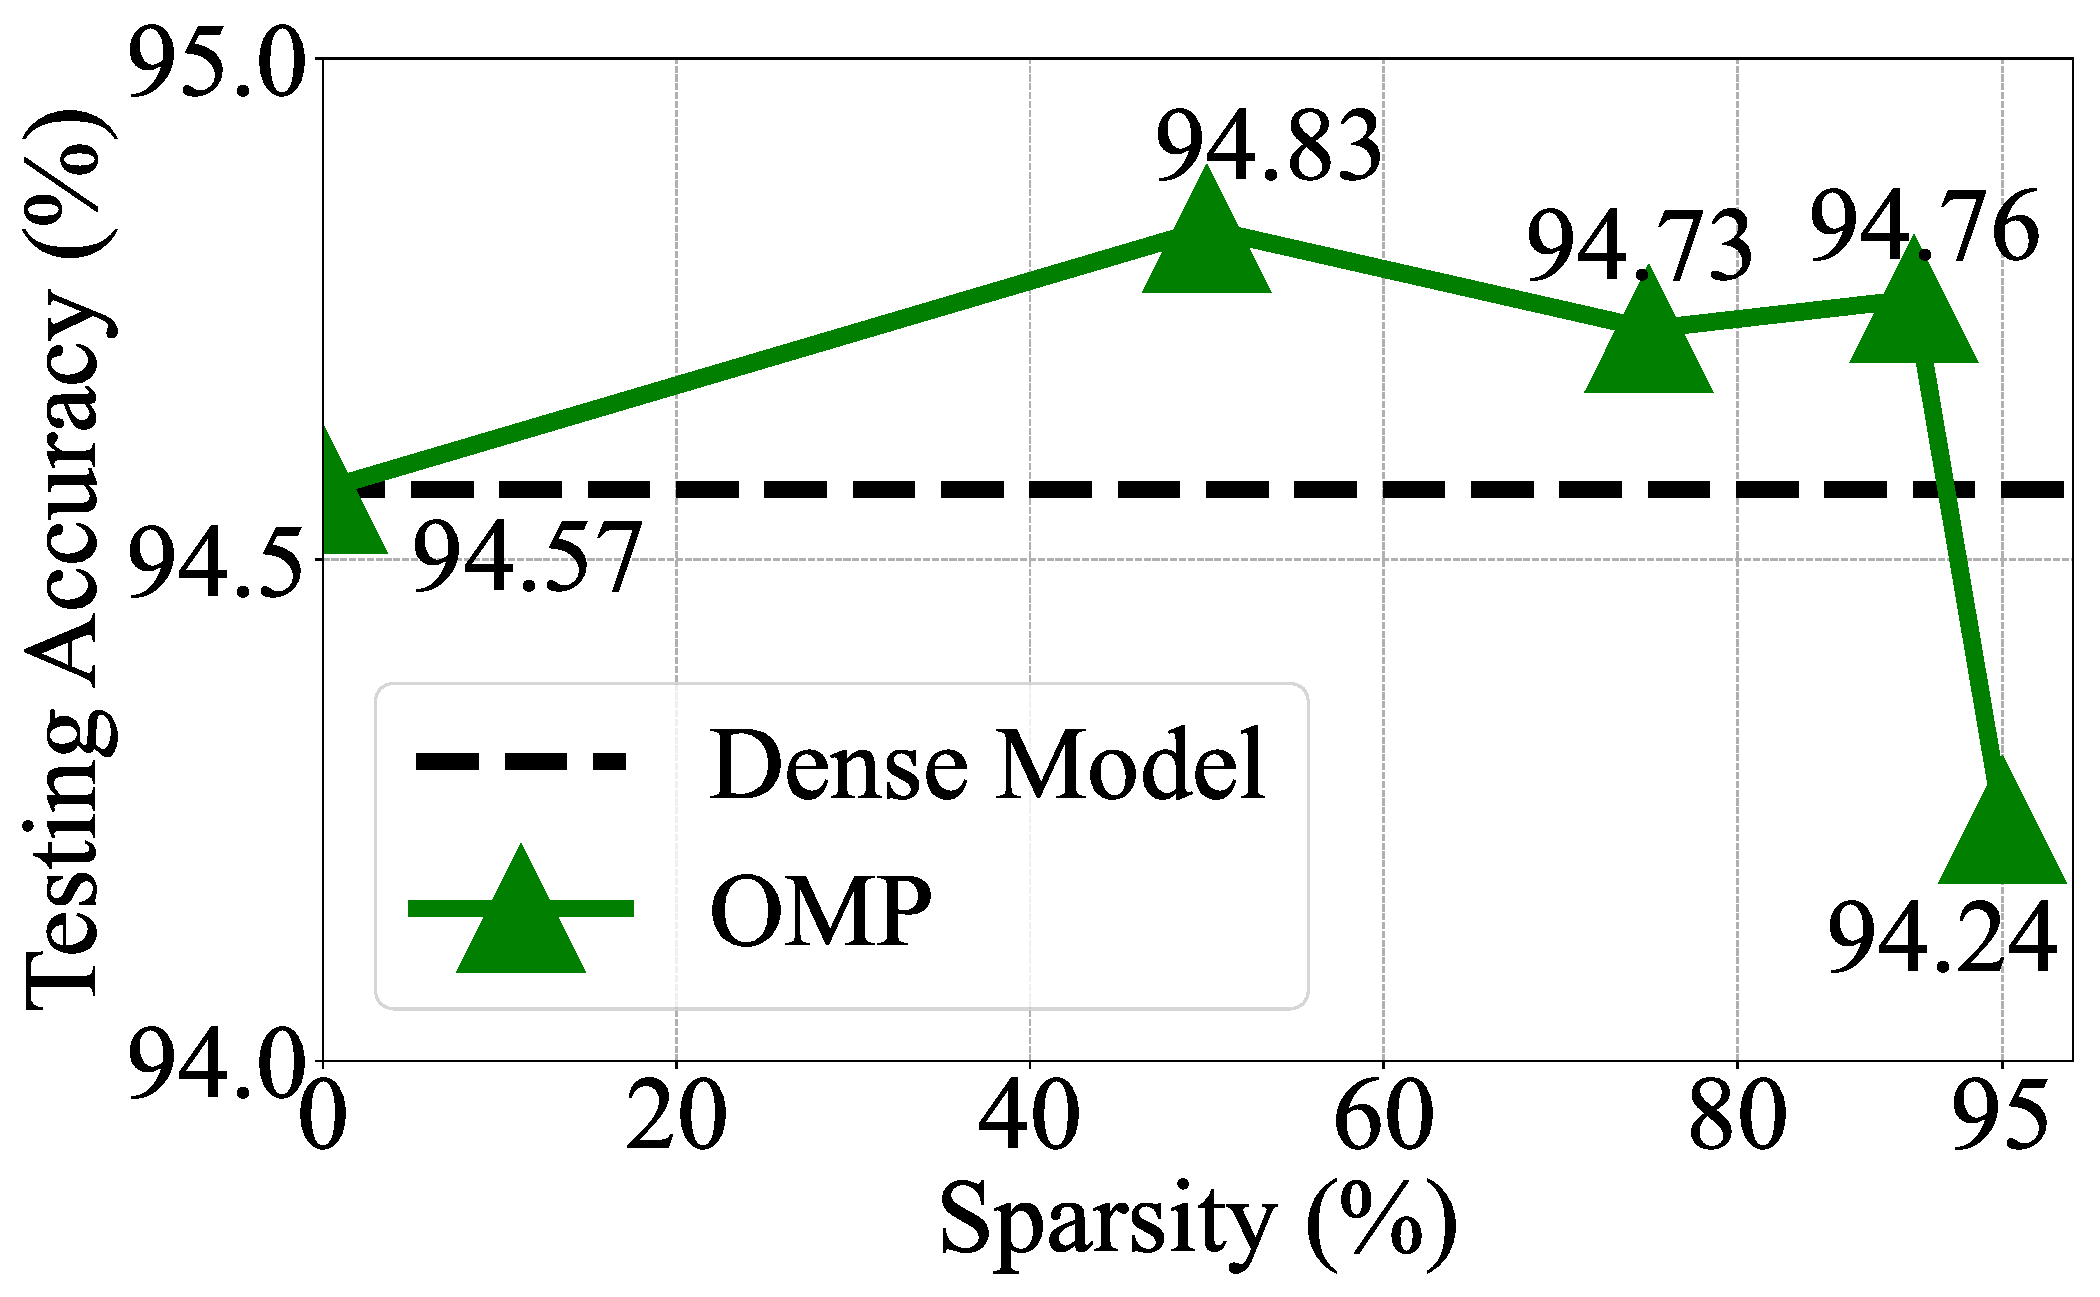
\includegraphics[width=45mm,height=!]{figs/OMP_on_CIFAR-10_ResNet18.pdf}
}
\vspace*{-2mm}
\caption{\footnotesize{
{Testing accuracy  of   OMP-based sparse ResNet-18   vs. the   dense model on CIFAR-10. 
%The  line  represents the mean  of test accuracies over 5 independent trials.
}
}}
  \label{fig: OMP_results}
 \vspace*{-5mm}
\end{wrapfigure}
\noindent \textbf{Gains of {\MU} from sparsity.}
We first analyze the impact of model sparsity on {\MU}  through a lens of   \textit{unrolling stochastic gradient descent} (\textbf{SGD}) \cite{thudi2021unrolling}. The specified SGD method allows us to derive the \textit{unlearning error} (given by the  weight difference between the approximately unlearned model   and the
gold-standard retrained model)  when scrubbing a single data point. However, different from \citet{thudi2021unrolling}, we  will infuse the model sparsity into  SGD unrolling. 


Let us assume a binary mask $\mathbf m$ associated with the model parameters $\btheta$, where $m_i = 0$ signifies that the $i$th parameter 
 $\theta_i$ is pruned to zero and $m_i = 1$  represents the unmasked   $\theta_i$.  This sparse pattern $\mathbf m$ could be obtained by a weight pruning method, like OMP. 
 %in Fig.\,\ref{fig: OMP_results} 
 %\PS{why refer to fig 2 here?}. 
Given $\mathbf m$,   the \textbf{sparse model}  is $ \mathbf m \odot \btheta $, where $\odot$ denotes the element-wise multiplication. Thudi \emph{et al.}\,\cite{thudi2021unrolling} showed that if 
%$\btheta^\prime = \btheta$ (\textit{i.e.}, $\mathbf{m} = \mathbf 1$) and  
{\GA} is adopted to scrub a single data point for the original (dense) model $ \btheta$ (\textit{i.e.}, $\mathbf{m} = \mathbf 1$),  then  the gap between {\GA} and {\retrain} can be approximately bounded in the weight space. 
  \textbf{Prop.\,\ref{prop: SGD_sparse_MU}} extends the existing unlearning error analysis   to a    sparse model. 

%error $e$ (\textit{i.e.}, the  weight difference from  {\retrain}) can be  bounded by

\iffalse 
\vspace*{-5mm}
{\small \begin{align}
   \hspace*{-2mm} e(\btheta_0, \{ \hat{\mathbf z}_i \},  t, \eta) 
 %\nonumber \\
=  \eta^2 \sum_{i=1}^{t-1} [ \nabla_{\btheta,\btheta}^2\ell(\btheta_0, \hat{\mathbf z}_i ) \sum_{j=0}^{i-1}   \nabla_{\btheta} \ell(\btheta_0, \hat{\mathbf z}_j ) ],
 \hspace*{-3mm}
 \label{eq: err_MU_SGD}
\end{align}}%
where $\btheta_0$ is  model initialization when using SGD-based ERM training,    $\{ \hat{\mathbf z}_i \}$
is the sequence of stochastic data samples, $t$ is the number of training iterations, $\eta$ is the learning rate, $\nabla_{\btheta,\btheta}^2\ell(\btheta_0, \hat{\mathbf z}_j)$ is the stochastic Hessian of the training loss $\ell$ evaluated at $\btheta_0$ and the  sample $\hat{\mathbf z}_j$.
Built upon \eqref{eq: err_MU_SGD}, 
%In the following 
Prop.\,\ref{prop: SGD_sparse_MU}  shows the    unlearning error   of {\GA} on a sparse model.
\fi 

%\SL{[Updated prop. Please check.]}
\begin{myprop}
\label{prop: SGD_sparse_MU}
Given the model sparse pattern $\mathbf m$ and the SGD-based  training, the unlearning error   of  {\GA}, denoted by $e(\mathbf m)$, can be characterized by the weight distance
between the {\GA}-unlearned model and the gold-standard retrained model. This leads to the error bound
\iffalse 
and 
 \underline{$ e_{\Omega_{\mathbf m}}(\btheta_0, \{ \hat{\mathbf z}_i \},  t, \eta) $}, where
 $e_{\Omega_{\mathbf m}}$ 
signifies the subvector of $e$ in \eqref{eq: err_MU_SGD} with coordinates given by the unmasked index set $\Omega_m$,  and $\Omega_{\mathbf{m}} = \{ i: m_i = 1 \}$ is the index set of unmasked parameters.
\fi 
%
% \vspace*{-5mm}
% {\small\begin{align}
%   \|  e^\prime(\btheta_0^\prime, \{ \hat{\mathbf z}_i \},  t, \eta)  \|_2 =
%   \|  e_{\Omega_{\mathbf m}}(\btheta_0, \{ \hat{\mathbf z}_i \},  t, \eta) \|_2 ,
%   \label{eq: MU_err_m}
% \end{align}}
% where $\btheta_0^\prime = \mathbf m \odot \btheta_0$,
% $\Omega_{\mathbf{m}} = \{ i: m_i = 1 \}$ is the index set of unmasked parameters, {\color{cyan}and  $e_{\Omega_{\mathbf m}}$ refers to the subvector of $e$ in \eqref{eq: err_MU_SGD} with coordinates given by the unmasked index set $\Omega_m$.}
%
%And the Euclidean norm of the unlearning error can be approximately bounded by
%modifies \eqref{eq: err_MU_SGD} to 
%\begin{align}
\iffalse
  $  e^\prime(\btheta_0^\prime, \{ \hat{\mathbf z}_i \},  t, \eta) \Def \mathbf m \odot e(\btheta_0, \{ \hat{\mathbf z}_i \},  t, \eta) $, where $e$ is  defined in  \eqref{eq: err_MU_SGD}.  
  \fi 
%\end{align}
%$\mathbf m \odot e(\btheta_0, \{ \hat{\mathbf z}_i \},  t, \eta) $. 
%an approximate     upper bound of the above  error is  given by
% \begin{align}
%     e(\mathbf m, \btheta_0, \{ \hat{\mathbf z}_i \},  t, \eta) 
% \end{align}

\vspace*{-5mm}
{\small\begin{align}
  % \|   e_{\Omega_{\mathbf m}}(\btheta_0, \{ \hat{\mathbf z}_i \},  t, \eta)  \|_2 
  e(\mathbf m) = \mathcal{O}(\eta^2 t  \| 
   \mathbf m \odot (\btheta_t - \btheta_0) \|_2 \sigma(\mathbf m) )
  % \leq \frac{\eta}{2}{(t-1) \|    \mathbf m \odot (\btheta_t - \btheta_0) \|_2}  \sigma(\mathbf m),
   \label{eq: err_bd_SGD_sparse}
\end{align}}%
where $\mathcal O$ is the big-O notation, $\eta$ is the learning rate, 
$t$ is the number of   training iterations, 
$ (\btheta_t - \btheta_0)$ denotes the weight difference at iteration $t$ from its   initialization $\btheta_0$,  and
$\sigma(\mathbf m)  $ is the largest singular value ($\sigma$) of the  Hessian $\nabla_{\btheta,\btheta}^2\ell$ (for a training loss $\ell$)   among the  unmasked parameter dimensions, \textit{i.e.}, $\sigma(\mathbf m) \Def \max_{j} \{  \sigma_{j}( \nabla_{\btheta,\btheta}^2\ell ), \text{if } m_j \neq 0  \}$.
%Here   $\sigma_j (\mathbf A)$ is the $j$th singular value of a matrix $\mathbf A$.

\textbf{Proof}: 
See Appendix\,\ref{appendix: SGD_sparse_MU}. 
%\SL{[ @Pranay, @Jinghan, @Jiancheng. Please check and use the above notations to complete the proof in appendix]}
\hfill $\square$
\end{myprop}
% \begin{myprop}
% \label{prop: SGD_sparse_MU}
% Given the model sparse pattern $\mathbf m$ and the SGD-based  training over the non-zero model weights in $\btheta^\prime$, the unlearning error of   {\GA} to scrub a single data point yields
% %modifies \eqref{eq: err_MU_SGD} to 
% %\begin{align}
%   $  e^\prime(\btheta_0^\prime, \{ \hat{\mathbf z}_i \},  t, \eta) \Def \mathbf m \odot e(\btheta_0, \{ \hat{\mathbf z}_i \},  t, \eta) $, where $e$ is  defined in  \eqref{eq: err_MU_SGD}.  
% %\end{align}
% %$\mathbf m \odot e(\btheta_0, \{ \hat{\mathbf z}_i \},  t, \eta) $. 
% An approximate     upper bound of the above  error is  given by
% % \begin{align}
% %     e(\mathbf m, \btheta_0, \{ \hat{\mathbf z}_i \},  t, \eta) 
% % \end{align}
% \begin{align}
%    \|   e^\prime(\btheta_0^\prime, \{ \hat{\mathbf z}_i \},  t, \eta)  \|_2 \leq \frac{\eta (t-1) \| \btheta_t - \btheta_0 \|_2}{2}  \sigma(\mathbf m),
%    \label{eq: err_bd_SGD_sparse}
% \end{align}
% where $\sigma(\mathbf m)  $ is the largest singular value of the stochastic Hessian $\nabla_{\btheta,\btheta}^2\ell$ given in \eqref{eq: err_MU_SGD} among the  model dimensions unpruned, \textit{i.e.}, $\sigma(\mathbf m) \Def \max_{j} \{  \sigma_{j}( \nabla_{\btheta,\btheta}^2\ell ), \text{if } m_j \neq 0  \}$. Here   $\sigma_j (\mathbf A)$ denotes the $j$th singular value of the matrix $\mathbf A$.
% \end{myprop}
We next draw some key insights   from \textbf{Prop.\,\ref{prop: SGD_sparse_MU}}. \textit{First},  it is clear from  \eqref{eq: err_bd_SGD_sparse} that the unlearning error reduces as the model sparsity in $\mathbf m$ increases. 
By contrast, the unlearning error  derived in  \citet{thudi2021unrolling} for a  dense model  (\textit{i.e.}, $\mathbf{m} = \mathbf 1$) is proportional to the dense model distance $\| \btheta_t - \btheta_0 \|_2$. 
%yields $O(\eta^2 t \| \mathbf{w}_t - \mathbf w_0 \|_2 \sigma(\mathbf 1))$.
%Recall that this unlearning error is given by the distance from the exact unlearned model.   
Thus,   model sparsity  is beneficial to reducing the gap between ({\GA}-based) approximate and exact unlearning. 
\textit{Second}, the error bound \eqref{eq: err_bd_SGD_sparse}  enables us to relate {\MU} to the  spectrum of the  Hessian  of the loss landscape. 
%Proposition\,\ref{prop: SGD_sparse_MU} that  the error term $\sigma(\mathbf m)$ in \eqref{eq: err_bd_SGD_sparse} characterizes the influence of model sparsity in {\MU}.  First, 
The number of active singular values (corresponding to nonzero dimensions in $\mathbf m$) decreases when the sparsity grows.
However, it is important to note that in a high-sparsity regime, the model's generalization   could   decrease. Consequently, it is crucial to  select the model sparsity to strike a balance between generalization   and unlearning performance.

% \SL{[Needs to clarify not  the sparser the better due to generalization loss.]}
% On the other hand, the magnitudes of these singular values also decrease since weight pruning can reduce the sharpness of the loss landscape; see  supporting  results in \textbf{Fig.\,\ref{fig: singular_sparsity}}.
%\SL{[Let us decide at the end if we should   move this to appendix.]}
%\PS{Is there a way to show this theoretically, since currently, in (4) we only observe decrease in number of active singular values.} 
% Such pruning effect has also been  justified by existing studies, \textit{e.g.},     %the reduced sharpness of the Hessian   \cite{chen2022can} and 
% the linear model connectivity of sparse models   \cite{frankle2020linear}. 
%The aforementioned insights from   \eqref{eq: err_bd_SGD_sparse}  also justify    that the unlearning error decreases as the sparsity of $\mathbf m$ increases; \PS{Isn't the last sentence redundant with first few sentences in this para?}


%Therefore, our key insight  from Proposition\,\ref{prop: SGD_sparse_MU} is that     model sparsity can contribute to reducing the gap between {\GA}-based approximate unlearning and exact unlearning. 

%the   error of  the {\GA}-based approximate unlearning method. 

%if the model is not pruned (\textit{i.e.}, $\mathbf m = \mathbf 1$), then 

%We provide some  insights   drawn from Proposition\,\ref{prop: SGD_sparse_MU} on the influence of model sparsity in {\MU}.  

% \begin{figure}[htb]
% %\begin{wrapfigure}{r}{80mm}
% %\vspace*{-6mm}
% \centerline{
% %\begin{tabular}{cc}
% %\hspace*{0mm}\includegraphics[width=.3\textwidth,height=!]{figure/performance_comparison.pdf}  
% %&
% %\hspace*{-4mm}
% \includegraphics[width=.31\textwidth,height=!]{example-image-a}
% % \\
% % \hspace*{2mm}\footnotesize{(a) Test accuracy vs. pruning ratio.} &   \footnotesize{(b) Runtime of pruning.}
% %\end{tabular}
% }
% \vspace*{-3mm}
% \caption{\footnotesize{
% TBD. 
% }}
%   \label{fig: singular_sparsity}
% %  \vspace*{-3.8mm}
% %\end{wrapfigure}
% %\end{figure}
% \end{figure}


\begin{figure*}[t]
% \vspace*{-3mm}
\centerline{
\begin{tabular}{cccc}
    \hspace*{-2mm}  \includegraphics[width=0.25\textwidth,height=!]{figs/ua.pdf} &
    \hspace*{-5mm} \includegraphics[width=0.25\textwidth,height=!]{figs/mia.pdf} &
    \hspace*{-5mm} 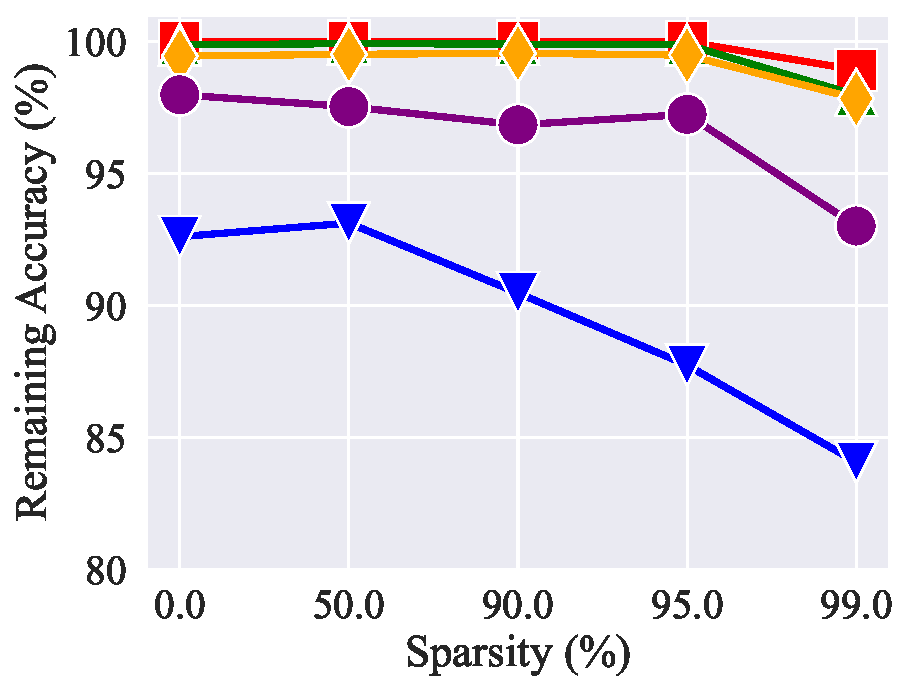
\includegraphics[width=0.25\textwidth,height=!]{figs/ra.pdf} &
    \hspace*{-5mm}  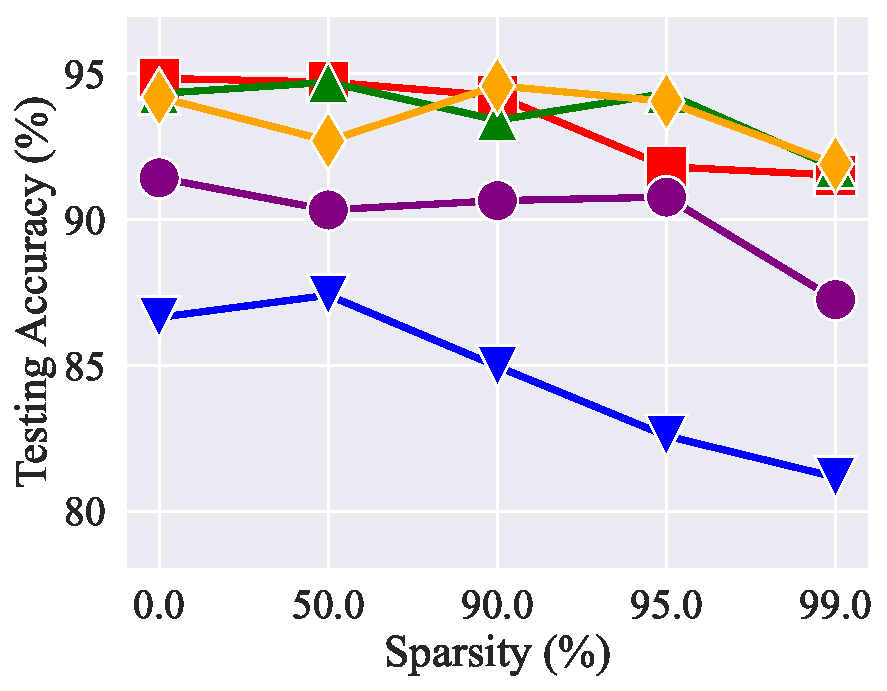
\includegraphics[width=0.25\textwidth,height=!]{figs/ta.pdf} 
\end{tabular}}
 \vspace*{-3mm}
\caption{\footnotesize{
%\SL{[Figure needs updating.]} %\JC{"Retain" -> "Remain"}
Performance of approximate unlearning ({\FTC}, {\GAC}, {\FFC}, {\IUC}) and exact unlearning ({\retrainC}) in efficacy ({\UA} and {\MIAF}), fidelity ({\RA}), and generalization ({\TA}) vs. model sparsity (achieved by {OMP}) in the data-model setup (CIFAR-10, ResNet-18). 
The unlearning scenario is class-wise 
 forgetting, and 
the average unlearning  performance over 10 classes is reported. We remark that being closer to \textcolor{red}{Retrain} performance is better for approximate MU schemes.
% \JC{TODO: Remove legend in fig 3c}
%\PS{See comment in the last para of Section 3. Are we trying to forget an entire class?}
}}
\vspace*{-7mm}
\label{fig: results_OMP_MU}
\end{figure*}

Inspired by Prop.\,\ref{prop: SGD_sparse_MU}, we ask: 
\textit{Does the above   benefit of model sparsification in {\MU} apply to   other approximate unlearning methods besides {\GA}?} This drives us to investigate the performance of approximate unlearning across the entire spectrum as depicted in  {Tab.\,\ref{tab: summary_MU_methods_metrics}}.
%unlearning on sparse models through our   multi-criteria evaluation in \textbf{Tab.\,\ref{tab: summary_MU_methods_metrics}}.
% conduct  the  all-dimension unlearning performance assessment 
% on sparse models, where evaluation metrics have been listed   in Table\,\ref{tab: summary_MU_methods_metrics}. 
Therefore,
\textbf{Fig.\,\ref{fig: results_OMP_MU}} shows the unlearning efficacy ({\UA} and {\MIAF}), fidelity ({\RA}), and generalization ({\TA}) of different   approximate unlearning methods   in the sparse model regime. Here class-wise forgetting is considered for {\MU} and OMP is used for weight pruning. 
% to 
% remove the influence of   all data points in one class from models pruned to different sparsity levels using OMP.
%\PS{We're trying to forget all the points from one class, right? This is not clear from this sentence.}
% on  OMP-based %\PS{``based''?}
% sparse models at different sparsity ratios. \PS{How about: ``... to remove the influence of all the data points belonging to a particular class from models pruned to different sparsity levels using OMP.''?}
%The performance of exact unlearning via {\retrain} is   provided for comparison. 
As we can see, the efficacy of approximate unlearning is significantly improved as the model sparsity increases, \textit{e.g.},   {\UA} and {\MIAF} of using {\FT} over 90\% sparsity.  By contrast, {\FT} over the dense  model (0\% sparsity) is the least effective for {\MU}. 
%\PS{Why do we mention FT alone? The same conclusion seems to hold for GA, FF, IU as well.}
%We also note that the efficacy  of {\retrain} is resilient to model sparsity. 
Also, the efficacy gap between exact unlearning ({\retrain}) and  approximate unlearning  reduces on sparse models. Further, through the fidelity and generalization lenses, {\FT} and {\FF} yield the {\RA} and {\TA}  performance closest to {\retrain}, compared to other unlearning methods. In the regime of ultra-high  sparsity (99\%), 
the efficacy of unlearning exhibits a tradeoff with  {\RA} and {\TA} to some extent.   
%For example, at the $95\%$-sparsity  regime, 

% presents our evaluation results  on {OMP}-based sparse models used in Fig.\,\ref{fig: OMP_results}. 
% % empirically study   the performance metrics  of   {\MU} methods  (Table\,\ref{tab: summary_MU_methods_metrics}) when applied to     sparse models given by OMP   in  Fig.\,\ref{fig: OMP_results}. Fig.\,\ref{fig: results_OMP_MU} shows our full-dimension assessments of {\MU} against model sparsity. 
% As we can see, \SL{[list key principled results.]}


% \begin{figure}[htb]
% \vspace*{-3mm}
% \centerline{
% \begin{tabular}{cccc}
%     \hspace*{-5mm}  \includegraphics[width=.23\textwidth,height=!]{figs/ua.pdf} &
%     \hspace*{-5mm} \includegraphics[width=.23\textwidth,height=!]{figs/mia.pdf} \\
    
%     \hspace*{-5mm} 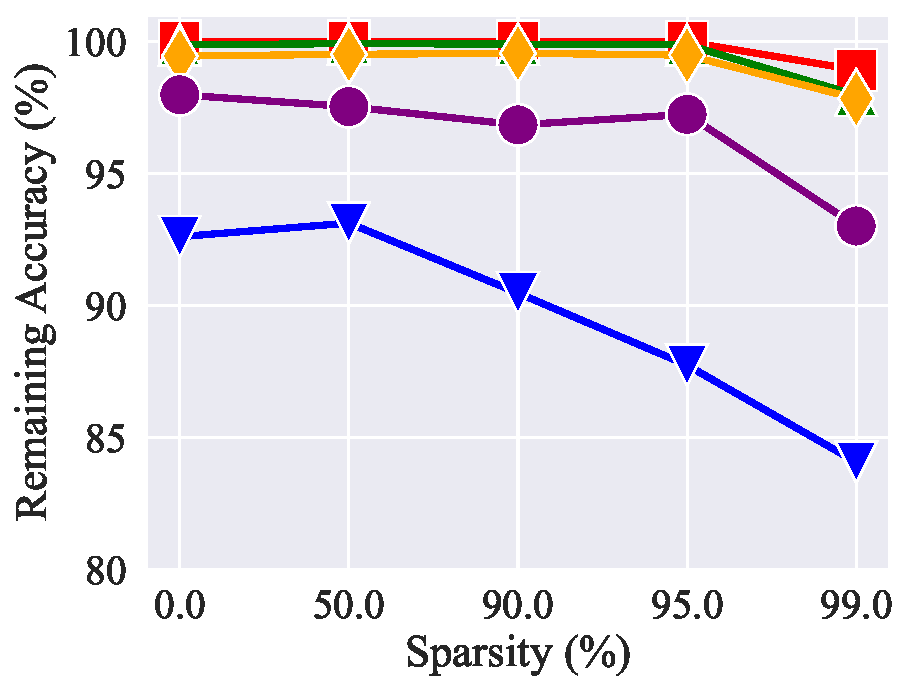
\includegraphics[width=.23\textwidth,height=!]{figs/ra.pdf} &
%     \hspace*{-5mm}  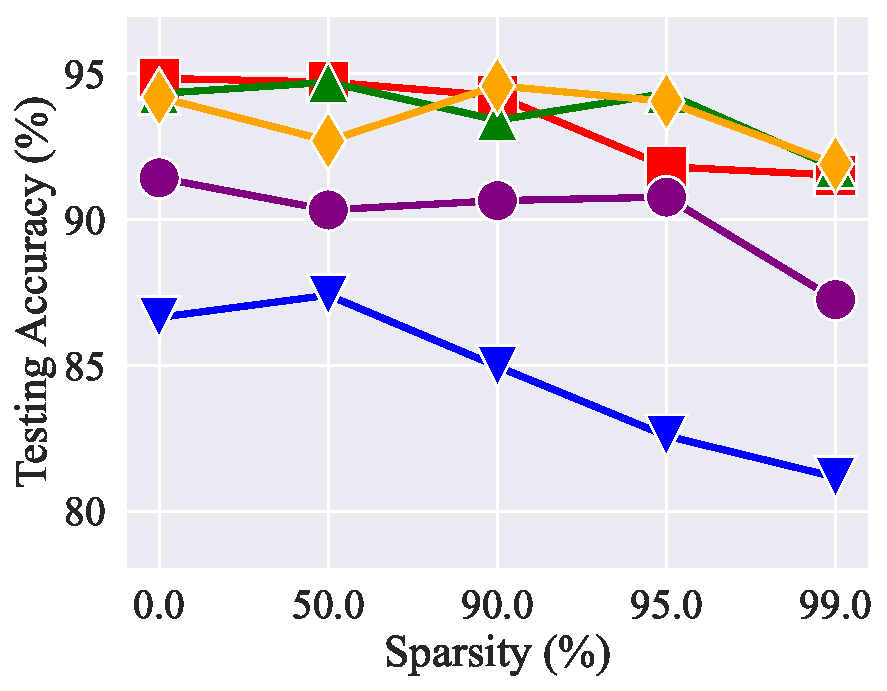
\includegraphics[width=.23\textwidth,height=!]{figs/ta.pdf} 
% \end{tabular}}
%  \vspace*{-3mm}
% \caption{\footnotesize{
% %\SL{[Figure needs updating.]} %\JC{"Retain" -> "Remain"}
% Performance of approximate unlearning ({\FTC}, {\GAC}, {\FFC}, {\IUC}) and exact unlearning ({\retrainC}) in efficacy ({\UA} and {\MIAF}), fidelity ({\RA}), and generalization ({\TA}) vs. model sparsity (achieved by {OMP}) in the data-model setup (CIFAR-10, ResNet-18). 
% The unlearning scenario is class-wise 
%  forgetting, and 
% the average unlearning  performance over 10 classes is reported. 
% %\PS{See comment in the last para of Section 3. Are we trying to forget an entire class?}
% }}
% % \vspace*{-3mm}
% \label{fig: results_OMP_MU}
% \end{figure}



\section{Sparsity-Aided Machine Unlearning}
\label{sec: sparsity_MU_alg}



%In the previous section, we showed that model sparsification could be a principled approach of reducing the gap between approximate unlearning and exact unlearning. 
Our study in Sec.\,\ref{sec: sparsityMU} suggests the new  {\MU} paradigm `prune first, then unlearn', which leverages the fact that  (approximate) unlearning on a sparse model yields a smaller unlearning error (Prop.\,\ref{prop: SGD_sparse_MU}) and improves the efficacy of {\MU}   (Fig.\,\ref{fig: results_OMP_MU}).
This promising finding, however, raises some new questions.  First, it remains elusive how the choice of a weight pruning method impacts the unlearning performance. Second,
%besides unlearning on a     sparse model,
it leaves room for developing  {sparsity-aware} {\MU} methods that can directly scrub data influence from a dense model.  %This section will address these two questions.
 



\noindent \textbf{Prune first, then unlearn: Choice of pruning methods.}
  % Our study in Sec.\,\ref{sec: sparsityMU} suggested the new  {\MU} paradigm `prune first, then unlearn', which shed light on that  (approximate) unlearning on a sparse model   yields a smaller unlearning error (Prop.\,\ref{prop: SGD_sparse_MU}) and improves the efficacy  of {\MU}   (Fig.\,\ref{fig: results_OMP_MU}).
  % Yet, 
  There exist many ways to find the desired sparse model
in addition to OMP. Examples include pruning at random
initialization before training \cite{tanaka2020pruning,frankle2020pruning}
 and simultaneous pruning-training iterative magnitude pruning (\textbf{IMP}) \cite{frankle2018lottery}.
  %Yet, there   exist many ways 
  %iterative magnitude pruning (\textbf{IMP}) \cite{ma2021sanity,frankle2018lottery}. 
  Thus, the problem of pruning method selection arises for {\MU}. From the viewpoint of {\MU},  the unlearner would prioritize a pruning method that satisfies the following criteria:  \ding{182} \textit{least dependence}  on the forgetting dataset ($\Df$), \ding{183} \textit{lossless generalization} when pruning, and \ding{184} \textit{pruning efficiency}. The rationale behind \ding{182} is  that  
  %since {\MU} targets scrubbing the influence of $\Df$ in the trained model, 
  it is desirable \textit{not} to incorporate    information of $\Df$ when seeking a sparse model prior to unlearning. 
  %\PS{This point is not clear to me. Additional info such as?} 
  And the criteria \ding{183} and \ding{184} ensure that sparsity cannot hamper {\TA} (testing accuracy)  and {\RTE} (run-time efficiency). 
  %which are also desired for {\MU} in addition to efficacy and fidelity (see Table\,\ref{tab: summary_MU_methods_metrics}).
  Based on \ding{182}-\ding{184}, 
  we   propose to use two pruning methods.  
  %in the `prune first, then unlearn' paradigm. 

\noindent  \ding{70} \textbf{SynFlow} (synaptic flow pruning) \cite{tanaka2020pruning}: 
SynFlow provides a (training-free) pruning method at initialization, even without   accessing the dataset. %to identify highly sparse sub-models  at initialization. 
Thus, it is uniquely suited for {\MU} to meet  the criterion \ding{182}. And SynFlow is easy to compute and yields a generalization improvement over many other pruning-at-initialization methods; see justifications in \cite{tanaka2020pruning}.


  
\noindent \ding{70} \textbf{OMP} (one-shot magnitude pruning)  \cite{ma2021sanity}: 
Different from SynFlow, {OMP}, which we focused on in Sec.\,\ref{sec: sparsityMU},
is performed over the original model   ($\thetafull$). It may depend on
%relate to \PS{``depend on''?}
%and thus  relates to 
the forgetting dataset ($\Df$), but has a much weaker dependence compared to {IMP}-based methods.
%Yet, such a relationship is much looser than     {IMP}-based methods \cite{frankle2018lottery}.
%that we have introduced and used in Sec.\,\ref{sec: sparsityMU} 
Moreover, {OMP} is  computationally lightest (\textit{i.e.}  best for \ding{184}) and    can yield better generalization than {SynFlow} \cite{zhang2022advancing}.
%Fig.\,\ref{fig: OMP_results} and Fig.\ref{fig: results_OMP_MU}


\begin{wrapfigure}{r}{72mm}
\vspace*{-4.5mm}
\centerline{
\begin{tabular}{cccc}
\hspace*{-5mm} 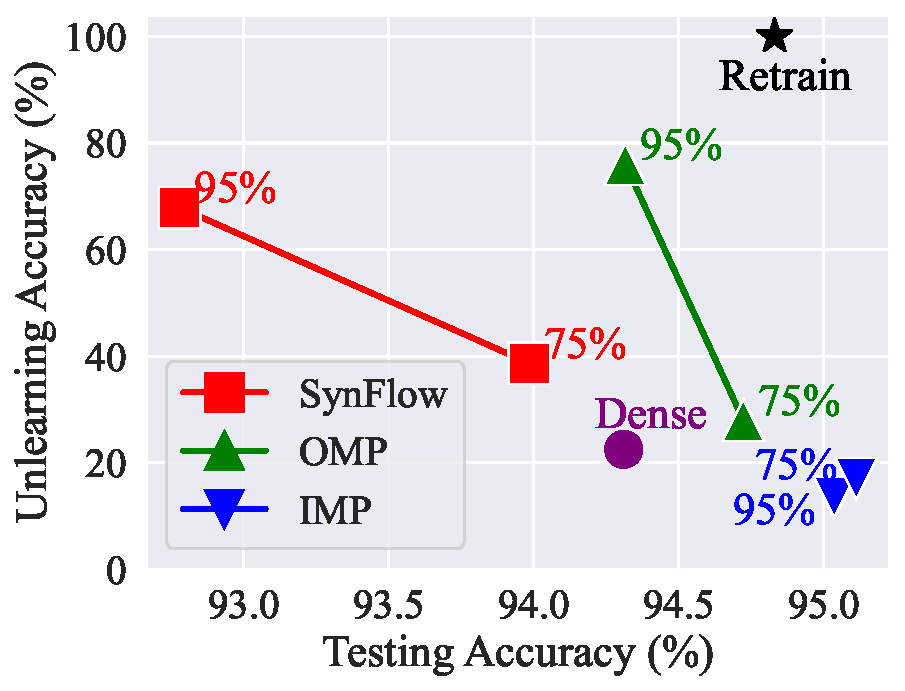
\includegraphics[width=35mm,height=!]{figs/UA_vs_pruning_retrain.pdf} &
    \hspace*{-5mm}  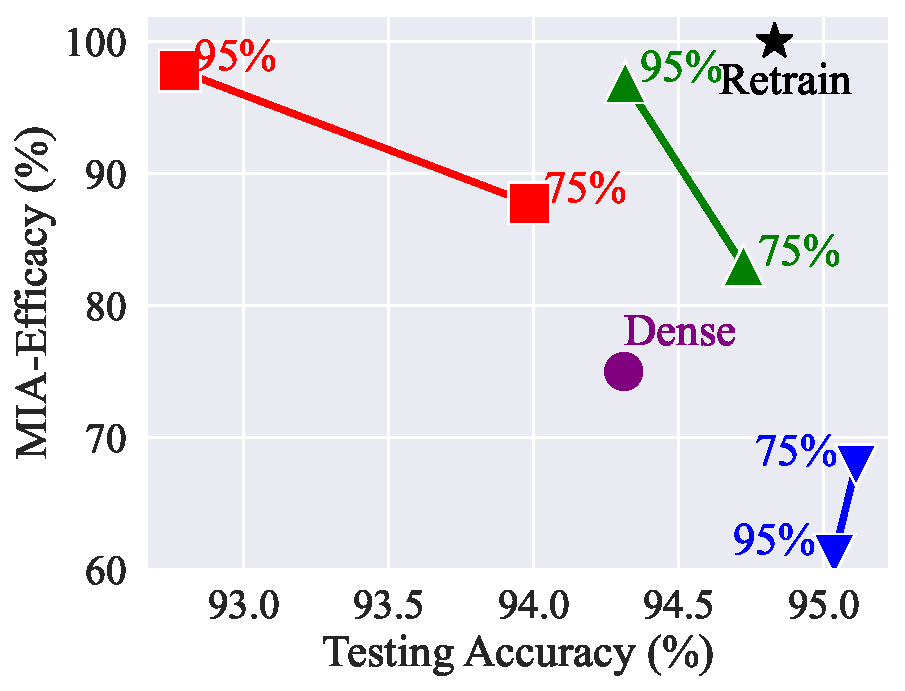
\includegraphics[width=35mm,height=!]{figs/MIA_vs_pruning.pdf} 
    \hspace*{-3mm} 
\end{tabular}}
 \vspace*{-3mm}
\caption{\footnotesize{Influence of different   pruning
methods ({\color{red}{SynFlow}}, {\color{ForestGreen}{OMP}}, and {\color{blue}{IMP}}) in unlearning efficacy ({\UA} and {\MIAF}) and generalization ({\TA})  on    (CIFAR-10, ResNet-18). \textbf{Left}: {\UA} vs. {\TA}. \textbf{Right}:   {\MIAF} vs. {\TA}. Each point is a {\FT}-based unlearned dense or sparse model (75\% or 95\% sparsity), or a retrained dense model.
%using  {\FT}. \JC{If a pruning method is proper for {\MU}, then its integration with {\FT} should  yield unlearned models with closer {\UA}, {\MIAF}, and {\TA} to {\retrain}.} 
%\JC{larger font in figs}
}}
 \vspace*{-4mm}
\label{fig: results_pruning_comparison}
\end{wrapfigure}
Furthermore, it is important to clarify that IMP (iterative magnitude pruning) is \textit{not} suitable for {\MU}, despite being widely used to find the most accurate sparse models (\textit{i.e.}, best for criterion \ding{183}).
% Next, we would like to highlight that IMP is not proper for {\MU} although it is the predominant approach to find the most accurate sparse models (\textit{i.e.},     best for \ding{183}). 
 % We also remark that in the research on model pruning, IMP   is   the predominant approach to find the most accurate sparse models (\textit{i.e.},     best for \ding{183}). 
 Compared with the proposed pruning methods, IMP has the largest computation overhead   and the strongest correlation with the training dataset (including $\Df$), thereby deviating from \ding{182} and \ding{184}.
 %due to its pruning-retraining iterations. 
 % In this sense, IMP may not be a proper  pruning choice for {\MU} through the lenses of \ding{182} and \ding{184}. 
 In \textbf{Fig.\,\ref{fig: results_pruning_comparison}}, we show  the   efficacy  of {\FT}-based unlearning on sparse models generated  using  different pruning methods (SynFlow, OMP, and IMP). 
 %where {\FF} is used as the unlearning algorithm.
 %the unlearning setup remains the same as Fig.\,\ref{fig: results_OMP_MU}.  
 As we can see, unlearning on {SynFlow} or {OMP}-generated sparse models yields improved {\UA} and {\MIAF} over that on the original dense model and   {IMP}-generated sparse models.  This unlearning improvement over the dense model is consistent with Fig.\,\ref{fig: results_OMP_MU}. More interestingly, we find that {IMP} \textit{cannot} benefit the unlearning efficacy, although it leads to the best {\TA}. This is because {IMP} heavily relies on the training set including forgetting data points, which is revealed by the empirical results -- the unlearning metrics get worse for IMP with increasing sparsity.
 %\textit{i.e.}, violating the criterion \ding{182}. 
 %We will  show a fix to {IMP} for {\MU} later.
 Furthermore, when examining the performance of SynFlow and OMP, we observe that the latter   generally outperforms the former, exhibiting results that are closer to those of {\retrain}. 
 %in {\TA} with  similar unlearning efficacy.  
 Thus,  \textit{{OMP} is the pruning method we will use by default}. 
 
 
 %at the model sparsity ratios 75\% and 95\%
 
 %compared to SynFlow and IMP, 
 
 %\SL{[add experiment analysis and distilled unlearning principles/insights. @Jiancheng, @Jinghan]}



%% While IMP is powerful, it requires multiple cycles of
%expensive training and pruning with very specific sets of hyperparameters.


%%% empirical results



%To this end, we  propose two sparsity-aware (approximate) unlearning methods below.

%built upon sparsity-regularized optimization   and pruning-unlearning alternative optimization (AO), respectively.  

%
\begin{wrapfigure}{r}{35mm}
\vspace*{-3mm}
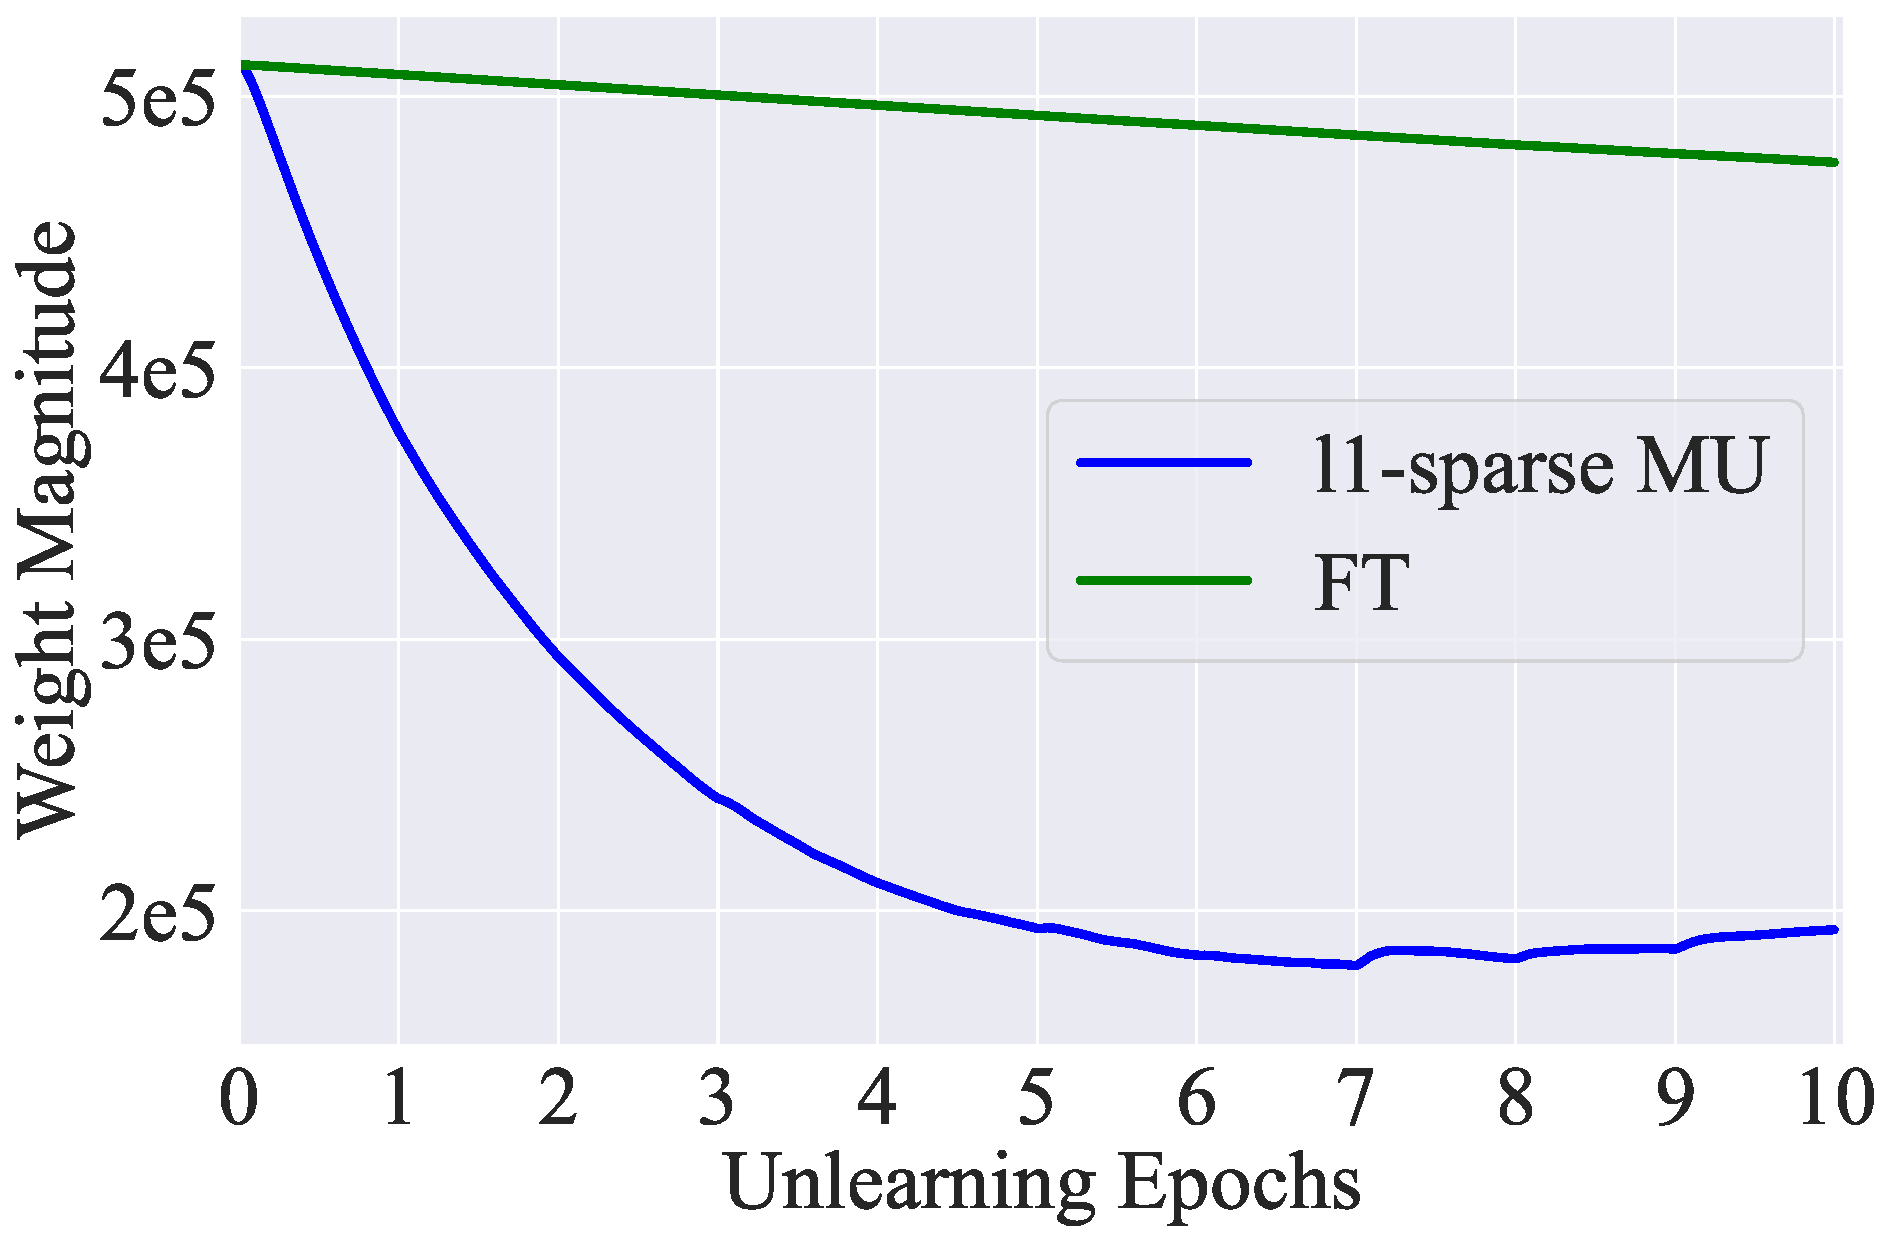
\includegraphics[width=35mm,height=!]{figs/magnitude.pdf}
\caption{\JC{Magnitude trend of the model weights during unlearning.}
\SL{Move to an appendix or delete.}}
\label{fig: l1_weight_magnitude}
\vspace*{-3mm}
\end{wrapfigure}
{\noindent \textbf{Sparsity-aware  unlearning.}}
% \JH{Add discussion about schedulers of $\gamma$, refer to table\,\ref{tab: ablation_l1_scheduler}.Also add some figures to show changes of magnitude.}
%In the   `prune first, then unlearn' paradigm, model sparsity is given \textit{a priori} for {\MU}. 
We next study if pruning and unlearning can be carried out simultaneously, without requiring prior knowledge of model sparsity. Let $\Lunl (\btheta; \thetafull,  \Dr)$ denote the unlearning objective function of model parameters $\btheta$, given the pre-trained  state $\thetafull$, 
%the overall training dataset $\mathcal D$, 
and the remaining training dataset $\Dr$. %Recall that $\Lunl $ can be specified by any {\MU} method studied in Sec.\,\ref{sec: primer_MU}. 
Inspired by  sparsity-inducing optimization \cite{bach2012optimization}, we integrate an $\ell_1$ norm-based sparse penalty into  $\Lunl $. This leads to the problem of `\textbf{\MUSparse}':

\vspace*{-3mm}
{\small{\begin{align}
    \thetaunl = \argmin_{\btheta} \Lunl (\btheta; \thetafull,  \Dr) + \gamma \| \btheta \|_1,
    \label{eq: MUSparse}
\end{align}}}%
where we specify $\Lunl$ by the fine-tuning objective, and $\gamma > 0$ is a regularization parameter that {controls the penalty level of the $\ell_1$ norm, thereby reducing the magnitudes of `unimportant' weights.}

%\noindent \textbf{\JC{Ablation study on parameter scheduler in \MUSparse.}}
% However, as \citep{bach2012optimization} mentioned, the downside of $\ell_1$ regulation term will affect the is its loss  in {\RA} and {\TA} compared to {\FT} and {\retrain}. Therefore, we conducted a comprehensive study of the scheduler of $\lambda$ in {\MUSparse}. In \textbf{Tab.\,\ref{tab: ablation_l1_scheduler}}, we present the results of unlearning performance on different parameter schedulers: constant scheduler, linear growing scheduler, and linear decaying scheduler.
% It shows that the decaying $\gamma$ scheduler performs the best among all the schedulers. If we directly apply a constant $\lambda$ to {\MUSparse}, it will either get a low {\UA} with lower $\lambda$ (for $\lambda = 0$, the method reduces to {\FT}) or worse {\RA} and {\TA} 
%  under higher $\lambda$. In Tab.\,\ref{tab: ablation_l1_scheduler}, we picked a sweet point to get a balance between them. If we use the linear growing scheduler, which means the method focuses on the unlearning term first then moves the focus to sparsity. If we use the linear decaying scheduler, the method focuses on the unlearning term first then moves the focus to sparsity.
\iffalse
\begin{wraptable}{R}{80mm}
\centering
\vspace*{-4.25mm}
\caption{\footnotesize{{\MU} performance  comparison of using {\MUSparse} with different   sparsity schedulers of $\gamma$  in \eqref{eq: MUSparse} and using {\retrain}.  
The unlearning scenario is given by random data forgetting (10\% data points across all classes) on (ResNet-18, CIFAR-10).
%considering various unlearning scenarios on CIFAR10 dataset. The content format follows Tab.\,\ref{tab: overall_perfoamnce}.
%Bold numbers indicate the closest performance to {\retrain}, and
A performance gap  against \textcolor{blue}{{\retrain}} is provided 
%. The relative drop or improvement represented 
in (\textcolor{blue}{$\bullet$}).
}}
\label{tab: ablation_l1_scheduler}
% \vspace*{0.1in} % Requirements, do not delete.
\resizebox{0.57\textwidth}{!}{
\begin{tabular}{c|c|c|c|c|c}
\toprule[1pt]
\midrule
  {\MU}& {\UA} & {{\MIAF}}& {{\RA}} & {{\TA}} & {{RTE} (min)} \\ 

% \cline{3-10}

% \midrule
% \rowcolor{Gray}
% \multicolumn{6}{c}{Class-wise forgetting} \\
% \midrule
% {\retrain} & \textcolor{blue}{100.00} & \textcolor{blue}{100.00} & \textcolor{blue}{100.00} & \textcolor{blue}{94.83} & 43.23
% \\
% {\MUSparse} + constant $\gamma$ & 100.00 (\textcolor{blue}{0.00}) & 100.00 (\textcolor{blue}{0.00}) & 91.69 (\textcolor{blue}{8.31})	& 87.3 (\textcolor{blue}{7.53}) & 2.61
% \\
% {\MUSparse} +   growing $\gamma$  & 100.00 (\textcolor{blue}{0.00}) & 100.00 (\textcolor{blue}{0.00}) & 94.43 (\textcolor{blue}{5.57})	& 88.43 (\textcolor{blue}{6.40}) & 2.61
% \\
% {\MUSparse} +   decaying $\gamma$ & 100.00 (\textcolor{blue}{0.00}) & 100.00 (\textcolor{blue}{0.00}) & \textbf{98.99} (\textcolor{blue}{\textbf{1.01}})	& \textbf{93.40} (\textcolor{blue}{\textbf{1.43}}) & 2.61
% \\
% \midrule
% \rowcolor{Gray}
% \multicolumn{6}{c}{Random data forgetting (all classes)} \\
\midrule
{\retrain} & \textcolor{blue}{5.41} & \textcolor{blue}{13.12} & \textcolor{blue}{100.00} & \textcolor{blue}{94.42} & 42.15
\\
%  \FT & $6.83$ (\textcolor{blue}{$1.42$}) & $14.97$ (\textcolor{blue}{$1.85$})& $96.61$ (\textcolor{blue}{$3.39$})& $90.13$ (\textcolor{blue}{$4.29$})  & 2.33 
% \\		
% \IU & $2.03$ (\textcolor{blue}{$3.38$})&  $5.07$ (\textcolor{blue}{$8.05$})& $98.26$ (\textcolor{blue}{$1.74$})& $\textbf{91.33}$ (\textcolor{blue}{$\textbf{3.09}$}) & 3.22
% \\
{\MUSparse} + constant $\gamma$ & 6.60 (\textcolor{blue}{1.19}) & 14.64 (\textcolor{blue}{1.52}) & 96.51 (\textcolor{blue}{3.49})	& 87.30 (\textcolor{blue}{7.53}) & 2.53
\\

{\MUSparse} + linear growing $\gamma$  & 3.80 (\textcolor{blue}{1.61}) & 8.75 (\textcolor{blue}{4.37}) & 97.13 (\textcolor{blue}{2.87})	& 90.63 (\textcolor{blue}{3.79}) & 2.53
\\
{\MUSparse} + linear decaying $\gamma$ & \textbf{5.35} (\textcolor{blue}{\textbf{0.06}}) & \textbf{12.71} (\textcolor{blue}{\textbf{0.41}}) & \textbf{97.39} (\textcolor{blue}{\textbf{2.61}})	& {\textbf{91.26}} (\textcolor{blue}{\textbf{3.16}}) & 2.53
\\
\midrule
\bottomrule[1pt]
\end{tabular}
}
\vspace*{-4mm}
\end{wraptable}
\fi
\vspace{-5mm}
\begin{table}[htb!]
\centering
\caption{\footnotesize{{\MU} performance  comparison of using {\MUSparse} with different   sparsity schedulers of $\gamma$  in \eqref{eq: MUSparse} and using {\retrain}.  
The unlearning scenario is given by random data forgetting (10\% data points across all classes) on (ResNet-18, CIFAR-10).
%considering various unlearning scenarios on CIFAR10 dataset. The content format follows Tab.\,\ref{tab: overall_perfoamnce}.
%Bold numbers indicate the closest performance to {\retrain}, and
A performance gap  against \textcolor{blue}{{\retrain}} is provided 
%. The relative drop or improvement represented 
in (\textcolor{blue}{$\bullet$}).
}}
\label{tab: ablation_l1_scheduler}
\vspace*{1mm}
% \vspace*{0.1in} % Requirements, do not delete.
\resizebox{0.85\textwidth}{!}{
\begin{tabular}{c|c|c|c|c|c}
\toprule[1pt]
\midrule
  {\MU}& {\UA} & {{\MIAF}}& {{\RA}} & {{\TA}} & {{RTE} (min)} \\ 

% \cline{3-10}

% \midrule
% \rowcolor{Gray}
% \multicolumn{6}{c}{Class-wise forgetting} \\
% \midrule
% {\retrain} & \textcolor{blue}{100.00} & \textcolor{blue}{100.00} & \textcolor{blue}{100.00} & \textcolor{blue}{94.83} & 43.23
% \\
% {\MUSparse} + constant $\gamma$ & 100.00 (\textcolor{blue}{0.00}) & 100.00 (\textcolor{blue}{0.00}) & 91.69 (\textcolor{blue}{8.31})	& 87.3 (\textcolor{blue}{7.53}) & 2.61
% \\
% {\MUSparse} +   growing $\gamma$  & 100.00 (\textcolor{blue}{0.00}) & 100.00 (\textcolor{blue}{0.00}) & 94.43 (\textcolor{blue}{5.57})	& 88.43 (\textcolor{blue}{6.40}) & 2.61
% \\
% {\MUSparse} +   decaying $\gamma$ & 100.00 (\textcolor{blue}{0.00}) & 100.00 (\textcolor{blue}{0.00}) & \textbf{98.99} (\textcolor{blue}{\textbf{1.01}})	& \textbf{93.40} (\textcolor{blue}{\textbf{1.43}}) & 2.61
% \\
% \midrule
% \rowcolor{Gray}
% \multicolumn{6}{c}{Random data forgetting (all classes)} \\
\midrule
{\retrain} & \textcolor{blue}{5.41} & \textcolor{blue}{13.12} & \textcolor{blue}{100.00} & \textcolor{blue}{94.42} & 42.15
\\
%  \FT & $6.83$ (\textcolor{blue}{$1.42$}) & $14.97$ (\textcolor{blue}{$1.85$})& $96.61$ (\textcolor{blue}{$3.39$})& $90.13$ (\textcolor{blue}{$4.29$})  & 2.33 
% \\		
% \IU & $2.03$ (\textcolor{blue}{$3.38$})&  $5.07$ (\textcolor{blue}{$8.05$})& $98.26$ (\textcolor{blue}{$1.74$})& $\textbf{91.33}$ (\textcolor{blue}{$\textbf{3.09}$}) & 3.22
% \\
{\MUSparse} + constant $\gamma$ & 6.60 (\textcolor{blue}{1.19}) & 14.64 (\textcolor{blue}{1.52}) & 96.51 (\textcolor{blue}{3.49})	& 87.30 (\textcolor{blue}{7.12}) & 2.53
\\

{\MUSparse} + linear growing $\gamma$  & 3.80 (\textcolor{blue}{1.61}) & 8.75 (\textcolor{blue}{4.37}) & 97.13 (\textcolor{blue}{2.87})	& 90.63 (\textcolor{blue}{3.79}) & 2.53
\\
{\MUSparse} + linear decaying $\gamma$ & \textbf{5.35} (\textcolor{blue}{\textbf{0.06}}) & \textbf{12.71} (\textcolor{blue}{\textbf{0.41}}) & \textbf{97.39} (\textcolor{blue}{\textbf{2.61}})	& {\textbf{91.26}} (\textcolor{blue}{\textbf{3.16}}) & 2.53
\\
\midrule
\bottomrule[1pt]
\end{tabular}
}
\end{table}
In practice,  the unlearning performance could be sensitive to the choice of the sparse regularization parameter $\gamma$. To address this limitation, we propose the design of a sparse regularization scheduler. Specifically, we explore three schemes: (1) constant $\gamma$, (2) linearly growing $\gamma$ and (3) linearly decaying $\gamma$; see Sec.\,\ref{sec: exp_setup} for detailed implementations. Our empirical evaluation presented in \textbf{Tab.\,\ref{tab: ablation_l1_scheduler}} shows that the use of a linearly decreasing $\gamma$ scheduler outperforms   other schemes.  
This scheduler not only minimizes the gap in unlearning efficacy compared to {\retrain}, but also improves the preservation of {\RA} and {\TA} after unlearning. 
These findings suggest that it is advantageous to prioritize promoting sparsity during the early stages of unlearning and then gradually shift the focus towards enhancing fine-tuning accuracy on the remaining dataset $\Dr$.

% As Sec.\,\ref{sec: sparsity_MU_alg} pointed out, the downside of the $\ell_1$ regularization term is its suppression on {\RA} and {\TA} compared to {\FT} and {\retrain}. To facilitate this deficiency, we introduced a well-designed scheduler to $\gamma$, the parameter of the regularization term, and conducted a comprehensive ablation study on designing the scheduler. The results of unlearning performance with different parameter schedulers, constant, linearly increasing, and linearly decreasing schedulers, are presented in \textbf{Tab.\,\ref{tab: ablation_l1_scheduler}}.

% Directly applying a constant $\gamma$ to {\MUSparse} would either yield a low unlearning efficacy with lower $\gamma$ (for $\gamma = 0$, the method reduces to {\FT}) or degraded generalization performance under higher $\gamma$. In \textbf{Tab.\,\ref{tab: ablation_l1_scheduler}}, we have identified an optimal point that balances these metrics. Still, it cannot achieve as good performance as scheduled $\gamma$. The linearly increasing scheduler implies that the method initially emphasizes the unlearning term, then gradually shifts its focus towards sparsity. Conversely, the linearly decaying scheduler suggests that the focus initially lands on the sparsity, then gradually shifts to the unlearning term. The results reveal that the decaying scheduler outperforms all the others on both class-wise forgetting and random data forgetting, which aligned with the inspiration of the `prune first, then unlearn' paradigm. Therefore, the decaying scheduler will use in successive experiments except specified otherwise.

%controls the sparsity of the model parameters in $\btheta$.  
%In \eqref{eq: MUSparse},   \SL{we specify $\Lunl$ by the fine-tuning objective}.  
%leading to the {\FT}-oriented {\MUSparse}. 
% \JC{\textbf{Fig.}\,\ref{fig: l1_weight_magnitude} shows during the {\MUSparse}, the variation tendency of the magnitude among the epochs, compared with {\FT}.}
% \JC{Moreover, since the $\ell_1$ regularizer would dampen the model's generalization performance, in order to get a balance between the impact of two terms, we used a decaying parameter schedule to $\gamma$. For further analysis and ablation studies on the scheduler selection, please refer to Sec.\,\ref{sec: experiment_results}.}

%\JC{\textbf{Fig.}\,\ref{fig: l1_weight_magnitude} illustrates the variation in magnitude among the epochs during the {\MUSparse} process, in comparison with {\FT}.}





% \JC{Furthermore, as the $\ell_1$ regularizer may dampen the model's generalization performance, we employ a decaying parameter schedule for $\gamma$ to gain advantages from both of the two terms. For a more in-depth analysis and ablation studies on scheduler selection, please refer to Sec.\,\ref{sec: experiment_results}.}

% \JC{ablation study on scheduler}

 
 %\SL{[Mention what existing unlearning objectives to be integrated with above proposal?]}
% \JC{remove AO?}
% In addition to \eqref{eq: MUSparse}, we can integrate pruning with unlearning via alternating optimization (\textbf{AO}) taking inspiration from the IMP algorithm \cite{frankle2018lottery}. Yet, different from IMP,  we replace the optimization step of retraining non-zero weights with unlearning on non-zero model weights. We term the resulting  method `\textbf{\MUAO}' and summarize its pipeline (S1)-(S3) below. 
% \textbf{(S1)} \textit{Initialize} model     $\btheta = \thetafull$ and a  pruning   mask $\mathbf m = \mathbf 1$.
% \textbf{(S2)}   \textit{Prune} $p\%$ non-zero parameters in $\btheta$ per magnitude. Then, update $\mathbf m$ to a sparser mask.
% \textbf{(S3)}  \textit{Unlearn} $\Df$ on the sparse model $\mathbf m \odot \btheta$ using an approximate unlearning method (\textit{e.g.}, {\FT}) to update the non-zero model parameters and go back to (S2).
% The above procedure \textbf{(S1)}$\to$\textbf{(S2)}$\rightleftarrows$\textbf{(S3)}  
%  repeatedly prunes and unlearns the model over multiple rounds (assuming $k$ rounds). Similar to IMP in \cite{frankle2018lottery},  we adopt a progressive learning process, where  each round prunes $p^{1/k}$\% of the weights on top of the previous round ($p=20\%$ by default). However, different from IMP,  {\MUAO} is much lighter in computation since approximate unlearning in (S2) takes fewer computation overheads than   retraining non-zero model weights in IMP.  


\iffalse 
We integrate two efficient unlearning methods {\FT} and {\GA} with these two proposed sparse-aware unlearning methods. In what follows, we will only report the {\FT}, which outperforms {\GA} integrated with sparsity-aware methods (shown in Table\,\ref{} \JH{appendix}).    
 \SL{[Mention what existing unlearning objectives to be integrated with above proposal?]}
 \fi 

\vspace{-0.2cm}
\section{Experiment}\label{sec:exp}
\vspace{-0.2cm}
In this section, we present the experimental results to validate the effectiveness of the proposed BAT algorithm on benchmark datasets and compare it with state-of-the-art baseline methods. We also verify that both two components are helpful and necessary for BAT. The implementation of the BAT can be found via \url{https://anonymous.4open.science/r/benign-adv-77C5}.

\vspace{-0.2cm}
\subsection{Experimental Setup}
\vspace{-0.1cm}
%\jt{we can put baselines here.} \\
%\jt{implementation details, such as optimization method}
In this work, in order to demonstrate the 
merit of BAT, we conduct the experiments mainly on benchmark datasets CIFAR100~\cite{krizhevsky2009learning} and Tiny~ImageNet~\cite{le2015tiny}, which are relatively complex datasets (i.e., containing larger fractions of atypical samples). For both datasets, we study the algorithms under the model architectures ResNet and WideResNet (WRN)~\cite{he2016deep}. In this section, we only present the results of ResNet18 for CIFAR100 and ResNet32 for Tiny~ImageNet and leave the results on WRN in Appendix~\ref{app:exp}. As a fair comparison with BAT, we implement the baseline algorithms including PGD adversarial training~\cite{madry2017towards} as well as its most popular variant TRADES~\cite{zhang2019theoretically}. In addition, we include several recent algorithms: MART~\cite{wang2019improving} and GAIRAT~\cite{zhang2020geometry}, which also incorporate reweighting strategies into adversarial training. For BAT and all baseline methods, we run the algorithms using SGD~\cite{bottou2010large} for 160 epochs with the learning rate that starts from 0.1 and decays by 0.1 after the epoch 80 and 120. More implementation details can be found in Appendix~\ref{app:exp}.

\textbf{Performance on CIFAR100.} For a comprehensive comparison between different methods on CIFAR100, in the results from Table~\ref{Tab:results_cifar100}, we report the models' clean accuracy and adversarial accuracy against $l_\infty$-$8/255$ PGD attack~\cite{madry2017towards}, as well as their performance on the typical sample set and atypical sample set (as described in Section~\ref{sec:pre}). A more comprehensive robustness evaluation on different attacking methods (including CW~\cite{carlini2017towards} and Auto-Attack~\cite{croce2020reliable}) are presented in Appendix~\ref{app:exp}. For BAT, we report its performance when choosing its optimal hyperparameter: $\alpha = 1  ~\text{\&} ~2$ and $\beta = 0.2$. In the Section~\ref{sec:ablation}, we will discuss the impact of the selection of $\alpha$ and $\beta$ on BAT. For baseline methods, the settings and checkpoint selections follow the original papers' suggestions.

%Note that the main goal of BAT is not to improve model's adversarial robustness, so we leave the robustness evaluation with additional attacking methods, such as CW~\cite{carlini2017towards} and Auto Attack~\cite{croce2020reliable} in  Appendix~\ref{app:exp} where we have similar observations.

\vspace{-0.3cm}
\begin{table}[h]
\small
\centering
\caption{Performance of BAT vs. Baselines on CIFAR100 Under ResNet18}
\begin{tabular}{c|cc|cc|cc}
\hline
Method & All Acc. & All Adv. & Typical Acc. & Typical Adv. & Atyp. Acc. & Atyp. Adv. \\
\hline
\hline
PGD Train (Best Adv.) & 56.9 & 27.4 & 90.6 & 59.0 &29.5 & 7.7\\
PGD Train (Best Clean) & 57.8 & 21.9 & 88.3 & 51.0 & \textbf{40.1} & 8.3 \\
%TRADES ($1/\lambda = 1$) & \textbf{61.3} & 21.9 & \textbf{93.0} & 50.0 & 44.7 & 7.9\\
TRADES ($1/\lambda = 5$) & 56.6 & 26.9 & 88.9 & 57.1 & 37.3 & \textbf{10.9} \\
MART~\cite{wang2019improving} & 51.8 & \textbf{30.4} & 85.3 & \textbf{62.2} & 25.3 & 10.1\\
GAIRAT~\cite{zhang2020geometry} & 58.2 & 27.8 & 90.6 & 60.7 & 31.6 & 8.2\\
\hline
BAT ($\alpha = 1, \beta = 0.2$) & \textbf{59.5} &27.3 & \textbf{92.3} & 58.8 & 36.3 & 8.7 \\
BAT ($\alpha = 2, \beta = 0.2$) &59.3 & 27.4 & \textbf{92.3} & 60.3 & 33.1 & 7.4 \\
\hline
\hline
\end{tabular}
\label{Tab:results_cifar100}
\end{table}
\vspace{-0.2cm}
From the results in Table~\ref{Tab:results_cifar100}, we can find that BATs enjoy good clean \& adversarial accuracy trade-off among all methods. It is because BATs can obtain the highest overall clean accuracy ($\sim59.5\%$), as well as comparably good adversarial accuracy ($\sim27.3$) with baseline methods. The only exception is MART~\cite{wang2019improving} which has the higher adversarial accuracy around $\sim 30\%$. However, MART~\cite{wang2019improving} has much lower clean accuracy than BATs. 

To gain a deeper understanding of the working mechanism of BAT, we focus on the performance on BAT vs. PGD adversarial training~\cite{madry2017towards}. Compared with PGD adversarial training with highest adversarial accuracy (PGD Train (Best Adv.)), the BAT methods are $2\sim3\%$ higher in terms of overall clean accuracy, and similar adversarial accuracy. The improvement of clean accuracy is mainly due to BATs' capacity to fit much more atypical samples. For example, the clean accuracy of BAT ($\alpha=1, \beta=0.2$) is about $6\%$ higher than PGD Train~(Best Adv.). On the other hand, compared to PGD adversarial training with the highest clean accuracy (PGD Train (Best Clean)), BATs have much better overall adversarial robustness and slightly better clean accuracy. This is mainly due to BAT's advantage on typical samples, because BATs can successfully prevent the performance drop of typical samples during the training process. Since BATs can achieve good performance on both typical samples and atypical samples, BATs outperform PGD adversarial training in CIFAR100.

\begin{wrapfigure}{r}{0.6\textwidth}
\vspace{-0.4cm}
\subfloat{
\begin{minipage}[c]{0.3\textwidth}
\centering
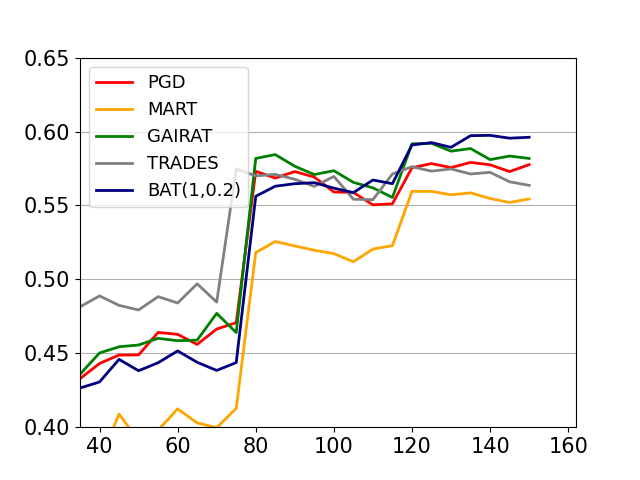
\includegraphics[width = 1.1\textwidth]{figures/base_clean.png}
\end{minipage}
}
\subfloat{
\begin{minipage}[c]{0.3\textwidth}
\centering
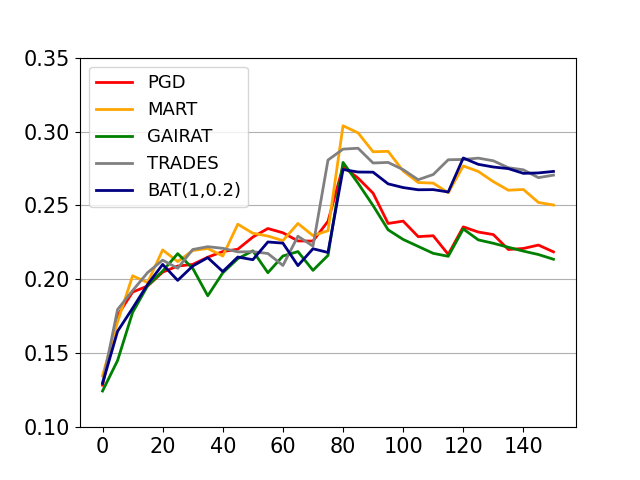
\includegraphics[width = 1.1\textwidth]{figures/base_rob.png}
\end{minipage}
}
\vspace{-0.4cm}
\caption{\small Clean Acc. (left) \& Adv. Acc (right)}
\label{fig:exp1}
\end{wrapfigure}
In Fig.~\ref{fig:exp1}, we also show the change of each models' overall clean accuracy (Fig~\ref{fig:exp1} (left)) \& adversarial accuracy (Fig~\ref{fig:exp1} (right)) along with the training progress. 
Interestingly, similar to PGD adversarial training, all baseline methods cannot achieve the optimal clean and adversarial accuracy at the same moment.
They always achieve the best adversarial accuracy around Epoch 80 (right after the first time weight decay), and the best clean accuracy on the last epochs. However, for BATs, since they can effectively prevent the robustness dropping in the late epochs, BATs are able to train until last epochs and enjoy good clean and adversarial accuracy simultaneously.
%As a result, BATs have higher clean accuracy than all baseline models, and good adversarial accuracy, which are similar or comparable to all baselines (even on their best checkpoints).

\textbf{Performance on Tiny~ImageNet.} Tiny~ImageNet~\cite{le2015tiny} contains 200 classes of the images in the original ImageNet~\cite{krizhevsky2012imagenet} dataset, with 500 training images for each class, and image size $64\times 64$. In our experiments, we only choose the first 50 classes in Tiny ImageNet for training and prediction. Since the image size is $64\times 64$, for both training and robustness evaluation, we consider the adversarial attacks are bounded by $l_\infty$-norm-4/255. In Table~\ref{Tab:results_imagenet}, we report the performance of BAT and baseline methods. Similar to the conclusions we can make from CIFAR100, BATs can achieve the highest overall clean accuracy and comparably good adversarial accuracy with baseline methods. 
\begin{table}[h]
\small
\vspace{-0.2cm}
\centering
\caption{Performance of BAT vs. Baselines on Tiny~ImageNet Under ResNet32}
\begin{tabular}{c|cc|cc|cc}
\hline
Method & All Acc. & All Adv. & Typical Acc. & Typical Adv. & Atyp. Acc. & Atyp. Adv. \\
\hline
\hline
Adv. Train (Best Adv.) & 56.3 & 32.3 & 97.5 & 85.3 &41.5 & 9.6\\
Adv. Train (Best Clean) & 58.2 & 30.5 & 98.0 & 80.4 & 44.7 & 9.1 \\
TRADES ($1/\lambda = 5$) & 55.4 & 28.8 & 97.3 & 77.4 & 38.8 & 9.6 \\
MART~\cite{wang2019improving} & 56.2 & \textbf{34.5} & 97.7 & 85.1 & 41.4 & \textbf{13.6} \\
GAIRAT~\cite{zhang2020geometry} & 58.4 & 30.4 & 98.0 & 81.7 & 45.7 & 7.8\\
\hline
BAT ($\alpha = 1, \beta = 0.2$) & \textbf{59.4} &32.0 & 98.4 & 83.9 & \textbf{48.4} & 10.2 \\
BAT ($\alpha = 2, \beta = 0.2$) &\textbf{59.4} &32.9 & \textbf{99.1} & \textbf{86.9} & 45.7 & 10.9 \\
\hline
\hline
\end{tabular}
\label{Tab:results_imagenet}
\end{table}

\vspace{-0.7cm}
\subsection{Ablation Study}\label{sec:ablation}
\vspace{-0.2cm}
\begin{wrapfigure}{r}{0.6\textwidth}
\vspace{-0.9cm}
\subfloat{
\begin{minipage}[c]{0.32\textwidth}
\centering
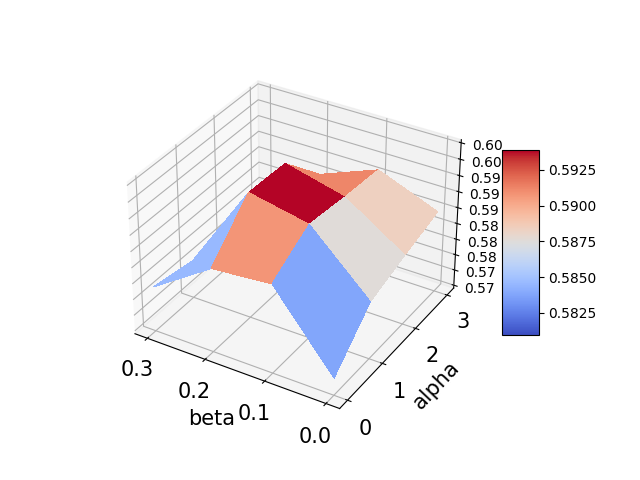
\includegraphics[width = 1.1\textwidth]{figures/abl_clean.png}
\end{minipage}
}
\subfloat{
\begin{minipage}[c]{0.32\textwidth}
\centering
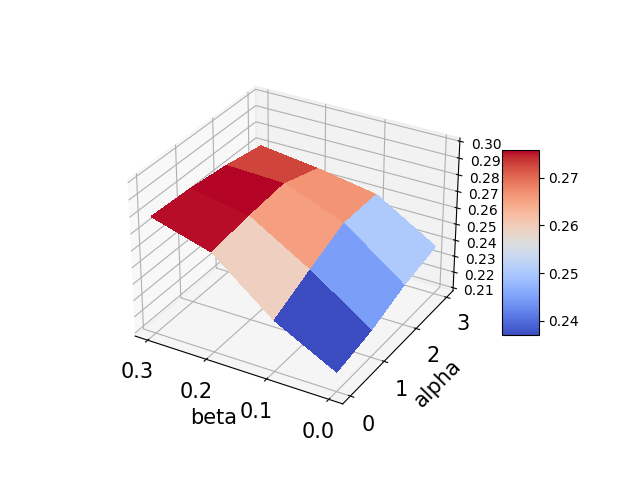
\includegraphics[width = 1.1\textwidth]{figures/abl_rob.png}
\end{minipage}
}
\caption{\small Clean Acc.(left) \& Adv. Acc.(right)}
\label{fig:exp2}
\vspace{-0.2cm}
\end{wrapfigure}
In this subsection, we study the potential impact of the hyperparameters chosen in BAT, which is $\alpha$ that controls the \textit{Reweighting} process and $\beta$ that controls the \textit{Discrimination Loss}. 
In Fig.~\ref{fig:exp2}, we conduct the experiments on CIFAR100 with BAT when $\alpha$ is chosen in [0,1,2,3] and $\beta$ is in [0, 0.1, 0.2, 0.3].
In Fig.~\ref{fig:exp2}, we show each model's overall clean accuracy~(left) \& adversarial accuracy~(right) along the Z-axis, and X-axis / Y-axis indicate the models' corresponding variables of $(\alpha,\beta)$. Note that when $\alpha=\beta=0$, the BAT method regresses to original PGD adversarial training. From the result, we can see that a positive pair of $(\alpha,\beta)$ can benefit both model clean and adversarial accuracy. Therefore, both two components \textit{Reweighting} and \textit{Discrimination Loss} of BAT are helpful and necessary. However, when $\alpha$ or $\beta$ is relatively too large, it will hurt the BAT's clean accuracy. As a result, in CIFAR~100, when $\alpha=1$ or 2 and $\beta= 0.2$, BAT can achieve the optimal performance.

%If we look at the performance of these models at their final epochs, we first observe that $\beta=0.2$ can improve both clean and adversarial accuracy, compared to all models with $\beta = 0$. Moreover, given any fixed value of $\beta$, the model with $\alpha = 1$ or 2 always outperforms than $\alpha=0$.
%Since a positive $\alpha$ indicates the BAT algorithm downweight or exclude certain samples during the training process, we can conclude that those  samples which are downweighted/excluded are acting like poisoning samples to deteriorate the models' performance. and necessary.

\section{Related Work}
\vspace*{-2mm}
% \JC{Ref Sec 2. more thorough related work }
While Sec.\,\ref{sec: primer_MU} provides a summary of related works concerning exact and approximate unlearning methods and metrics,  a more comprehensive review  is provided below.

\noindent \textbf{Machine unlearning.}
%% sparsity in unlearning.
\iffalse 
{\MU} was first introduced in   \cite{cao2015towards}, which aims to make  an ML model to `forget'  data points upon completion of training.   {\MU}  was originally used  to prevent the leakage of  data privacy  from the trained model,   
in particular in coming forth with legislation like  General Data Protection Regulation (GDPR) \cite{hoofnagle2019european} and  California Consumer Privacy Act (CCPA) \cite{pardau2018california}. 
A straightforward approach  to unlearning is to retrain the model from scratch (\textit{i.e.}, {\retrain}) after removing the forgetting dataset from the original training set. Although {\retrain} yields the ground-truth unlearning strategy, it is least efficient in computation. Thus,   approximate but fast unlearning    becomes a significant research focus nowadays; examples include \cite{golatkar2020eternal,warnecke2021machine,graves2021amnesiac,thudi2021unrolling,becker2022evaluating,izzo2021approximate} as we reviewed in Sec.\,\ref{sec: primer_MU}. 
\fi 
In addition to exact and approximate unlearning methods as we have reviewed in Sec.\,\ref{sec: primer_MU}, there  exists other literature aiming to  develop  the probabilistic notion of unlearning \cite{ginart2019making,guo2019certified,neel2021descent,ullah2021machine,sekhari2021remember}, in particular through the lens of differential privacy (DP) \cite{dwork2006our}. Although DP enables unlearning  with provable error guarantees, %\cite{guo2019certified,neel2021descent,ullah2021machine,sekhari2021remember}, 
they typically require strong model and algorithmic assumptions and could lack effectiveness when facing practical  adversaries, \textit{e.g.}, membership inference attacks. Indeed, evaluating {\MU}  is far from trivial \cite{becker2022evaluating,thudi2022necessity,thudi2021unrolling}.  %as we described in Sec.\,\ref{sec: primer_MU}. 
Furthermore, the attention on  {\MU} has also   been raised in   different learning paradigms, \textit{e.g.}, federated learning   \cite{wang2022federated,liu2022right}, graph neural networks \cite{chen2022graph,chien2022certified,cheng2023gnndelete}, and adversarial ML \cite{marchant2022hard,di2022hidden}.
In addition to   preventing the leakage of  data privacy  from the trained models, the concept of {\MU} has also inspired  other emergent applications such as adversarial defense against backdoor attacks \cite{liu2022backdoor,warnecke2021machine} that we have studied and erasing image concepts of conditional generative models \cite{gandikota2023erasing,zhang2023forget}.
%Moreover, in addition to its primary applications, we have demonstrated \MU's potential in mitigating backdoor attacks \cite{liu2022backdoor}, as well as in augmenting the performance of transfer learning \cite{jain2022data}. These diverse applications underscore the versatility and utility of machine unlearning in various domains.

 


\noindent \textbf{Understanding data influence.}
The majority of {\MU} studies are motivated by data privacy. Yet, they  also closely relate to another line of research on understanding data influence in ML. For example, the influence function approach \cite{koh2017understanding} has been used as an algorithmic backbone of many unlearning methods  \cite{warnecke2021machine,izzo2021approximate}. From the viewpoint of data influence, {\MU}  has been used in the use case of adversarial defense against data poisoning backdoor attacks \cite{liu2022backdoor}. Beyond unlearning, evaluation of data influence  has also been studied in  fair learning  \cite{sattigeri2022fair,wang2022understanding},  transfer learning  \cite{jain2022data}, and   dataset pruning \cite{borsos2020coresets,yang2022dataset}. 
%to improve  the efficiency of ML. 


% It can also be viewed as a method of understanding dataset influence
% %\PR{dataset influence?}
% in model training


%%  In [16], Liu et al., for instance, utilize forgetting in order to remove backdoors that were induced into a model.

\noindent \textbf{Model pruning.}
%\iffalse 
The deployment constraints on \textit{e.g.}, computation, energy, and memory   necessitate the pruning of
today's ML models, \textit{i.e.}, promoting their weight sparsity. %\cite{han2015deep,chen2021lottery,frankle2018lottery,frankle2020linear,ma2021sanity,zhang2022advancing}.
%\fi 
The vast majority of existing works \cite{han2015deep,chen2021lottery,frankle2018lottery,frankle2020linear,ma2021sanity,zhang2022advancing,blalock2020state} focus on  developing model pruning methods that can strike a graceful balance between model's generalization and sparsity.
%the  generalization ability of pruned models against its sparsity; see the seminal work \cite{blalock2020state}. 
In particular, the existence of LTH (lottery ticket hypothesis) \cite{frankle2018lottery} demonstrates 
the feasibility of co-improving the model's generalization  and efficiency (in terms of sparsity) \cite{liu2018rethinking,tanaka2020pruning,wang2020picking,lee2018snip,zhang2023data}. 
%has been empirically justified  by LTH (lottery ticket hypothesis) \cite{frankle2018lottery},
\iffalse 
This has inspired 
many different kinds of pruning methods \cite{liu2018rethinking,tanaka2020pruning,wang2020picking,lee2018snip}. 
\fi 
In addition to generalization, model sparsity   achieved by pruning   can also be  leveraged to improve other performance metrics, such as   robustness \cite{sehwag2020hydra,chen2022quarantine,diffenderfer2021winning}, model explanation  \cite{wong2021leveraging,chen2022can},
%model connectivity \cite{frankle2020linear}, 
and privacy \cite{huang2020privacy,wang2020against,luo2021scalable,gong2020privacy}.

\iffalse 
out-of-distribution generalization \cite{diffenderfer2021winning}. 
In particular, the   relevant work to ours is model pruning for privacy-preserving learning \cite{huang2020privacy,wang2020against,luo2021scalable,gong2020privacy}. Yet,  nearly all the existing works  focus on how sparsity impacts data privacy, \textit{e.g.}, evaluated using MIAs (membership inference attacks) 
%against pruned models on training data points 
\cite{bagmar2021membership,yuan2022membership}. This is akin to MIA evaluation on the retained dataset in our work. Thus, pruning for privacy cannot   provide   a holistic and in-depth understanding of  how pruning  impacts {\MU}.  
\fi 

\iffalse
In addition,
a few recent works   \cite{wang2022federated,ye2022learning} attempt to draw insights from pruning for unlearning. In \cite{wang2022federated},  pruning channels of a  neural network shows   unlearning benefits in federated learning. And in \cite{ye2022learning}, filter pruning is introduced in lifelong learning to detect pruning identified exemplars (PIEs)   \cite{hooker2019compressed} that  are easy to forget. 
Different from the aforementioned literature to customize  pruning   for specific unlearning applications,  our work for the first time explores and exploits the connection between model pruning and unlearning systematically and in-depth. 
\fi 


%or membership inference attack and defense 

%\textsc{Grasp}\,\cite{wang2020pick}, \textsc{Snip}\,\cite{lee2018snip}, 

%%% pruning vs. privacy
%\paragraph{Pruning for.}



\section{Conclusion}
In this work, we advance the method of {machine unlearning} through a novel viewpoint: model sparsification, achieved by weight pruning. We show in both theory and practice that model sparsity plays a foundational and crucial role in closing the gap between exact unlearning and existing approximate unlearning methods. Inspired by that, we propose two new unlearning paradigms,  `prune first, then unlearn' and `sparsity-aware unlearn', which can significantly improve the efficacy of approximate unlearning. We demonstrate the effectiveness of our findings and proposals in extensive experiments across different unlearning setups. Our study also indicates the presence of \textit{model modularity} traits, such as weight sparsity, that could simplify the process of machine unlearning. This may open up exciting prospects for future research to investigate unlearning patterns within weight or architecture space.





\section{Acknowledgement}

{The work of J. Jia, J. Liu, Y. Yao, and S. Liu were supported by the Cisco Research Award and partially supported by the NSF Grant IIS-2207052, and the ARO Award W911NF2310343. Y. Liu was partially supported by NSF Grant IIS-2143895 and IIS-2040800. }

{{
%\bibliographystyle{IEEEbib}
\bibliographystyle{unsrtnat}
\bibliography{bibs/ref_JC_attack,bibs/ref_jh_model_dataset,bibs/ref_SL_pruning,bibs/unlearning}
}}
\newpage
\clearpage
\appendix

% \setcounter{lemma}{0}
%     \renewcommand{\thelemma}{\Alph{section}\arabic{lemma}}
    
\begin{comment}
\end{comment}

{\colorred 
\section{Compatible Value Function}
\label{app:comp_v}

The original policy gradient with compatible value function is stated as follow. 
\begin{theorem}
[\cite{sutton1999policy}]
Let $Q_w$ be a state-action function with parameter $w$ and $\pi_\theta$ be a policy function with parameter $\theta$. 
If $Q_w$ satisfies $\mathbb{E}_{\pi} [(Q^\pi - Q_w) \nabla_w Q_w] = 0$ and 
$\nabla_w Q_w = \nabla_\theta \log \pi_\theta,$
then $$\nabla_\theta \mathcal{J} = \mathbb{E}_\pi [Q_w \nabla_\theta \log \pi_\theta].$$
\label{thm:pg_fa}
\end{theorem}
If we let $w = \theta$ in Theorem \ref{thm:pg_fa}, where $Q_w$ and $\pi_\theta$ share parameters, we have the following theorem. 
\begin{theorem}
Let $Q_\theta$ be a state-action function with parameter $\theta$ and $\pi_\theta$ be a policy function with parameter $\theta$. 
If $Q_\theta$ satisfies $\mathbb{E}_{\pi} [(Q^\pi - Q_\theta) \nabla_\theta Q_\theta] = 0$ and 
$\nabla_\theta Q_\theta = \nabla_\theta \log \pi_\theta,$
then $$\nabla_\theta \mathcal{J} = \mathbb{E}_\pi [Q_\theta \nabla_\theta \log \pi_\theta].$$
\label{thm:pg_fa2}
\end{theorem}
Define 
$$\chi \overset{def}{=} \mathbb{E}_\pi [\cos <\nabla_\theta Q_\theta, \nabla_\theta \log \pi_\theta>].$$
We show that $\chi = 1$ is the necessary condition for the compatible condition $\nabla_\theta Q_\theta = \nabla_\theta \log \pi_\theta$. 
\begin{theorem}
i) If $\nabla_\theta Q_\theta \propto \nabla_\theta \log \pi_\theta$ for all states, then $\chi = 1$.

ii) If $\chi = 1$, then $\nabla_\theta Q_\theta \propto \nabla_\theta \log \pi_\theta$ for all states. 
\label{thm:connect_cond}
\end{theorem}
By Theorem \ref{thm:connect_cond}, $\chi = 1$ is equivalent to $\nabla_\theta Q_\theta \propto \nabla_\theta \log \pi_\theta$, and $\nabla_\theta Q_\theta \propto \nabla_\theta \log \pi_\theta$ is the necessary condition for $\nabla_\theta Q_\theta = \nabla_\theta \log \pi_\theta$, hence $\chi = 1$ is the necessary condition for $\nabla_\theta Q_\theta = \nabla_\theta \log \pi_\theta$.
\begin{proof}
i) Since $\nabla_\theta Q_\theta \propto \nabla_\theta \log \pi_\theta$, we have $<\nabla_\theta Q_\theta, \nabla_\theta \log \pi_\theta> = 0$. 
By definition of $\chi$, we have 
$$\chi = \mathbb{E}_\pi [\cos <\nabla_\theta Q_\theta, \nabla_\theta \log \pi_\theta>] = \mathbb{E}_\pi [1] = 1.$$

ii) Since $\chi \leq 1$ and $\cos(x)$ is monotonic decreasing as $x$ goes from $0$ to $\pi$, the equality $\chi = 1$ only holds when all states satisfy $\cos <\nabla_\theta Q_\theta, \nabla_\theta \log \pi_\theta> = 0$, which means $\nabla_\theta Q_\theta \propto \nabla_\theta \log \pi_\theta$. 
\end{proof}
}

% $$
% \begin{aligned}
%     logp &= variable((3, 3, 4)) \\
%     q &= variable((3, 3, 4)) \\
%     alpha &= 0.3 \\
%     \pi &= softmax(alpha * logp + (1.0 - alpha) * q) \\
% \end{aligned}
% $$
\clearpage

\section{Gradients Between Policy Improvement and Policy Evaluation}
\label{app:mtv}

\begin{table}[hb!]
    \centering
    \scalebox{0.90}{
    \begin{math}
        \begin{array}{c|c|c|c}
    \toprule
     & \text{Function Approximation} & \text{Train Gradients} & \text{Cosine of Interested Angles} \\
    \midrule
    
    \text{PPO} & (V, logit) = (V_\theta, logit_\theta) & 0.5 \nabla L_V + \nabla \mathcal{J} & %\cos<\nabla L_V, \nabla \mathcal{J}> 
    \\ 
    & \pi = \text{softmax}(logit) & & \\
    
    \midrule
    
    \text{PPO ver.1} & (Q, logit) = (Q_\theta, logit_\theta), & 0.5 \nabla L_V + \nabla \mathcal{J} & \cos<\nabla L_Q, \nabla \mathcal{J}>%\cos<\nabla L_V, \nabla \mathcal{J}> 
    \\
    & \pi = \text{softmax}(logit) & & \cos<\nabla Q, \nabla \log \pi> \\
    & V = sg(\pi)\cdot Q & & %\cos<\nabla L_V, \nabla L_Q> 
    \\
    % & & &  \\
    
    \midrule
    
    \text{PPO ver.2} & (Q, logit) = (Q_\theta, logit_\theta), & 0.5 \nabla L_V + \nabla L_Q + \nabla \mathcal{J} & \cos<\nabla L_Q, \nabla \mathcal{J}> %\cos<\nabla L_V, \nabla \mathcal{J}> 
    \\
    & pi = \text{softmax}(logit) & & \cos<\nabla Q, \nabla \log \pi> \\
    & V = sg(\pi)\cdot Q & & %\cos<\nabla L_V, \nabla L_Q> 
    \\
    % & & &  \\
    
    \midrule
    
    \text{PPO+CASA} & (V, A) = (V_\theta, A_\theta), & 0.5 \nabla L_V + \nabla L_Q + \nabla \mathcal{J} & \cos<\nabla L_Q, \nabla \mathcal{J}> %\cos<\nabla L_V, \nabla \mathcal{J}> 
    \\
    & \pi = \text{softmax}(A/\tau), & & \cos<\nabla Q, \nabla \log \pi> \\
    & \Bar{A} = A - sg(\pi) \cdot A & & %\cos<\nabla L_V, \nabla L_Q> 
    \\
    & Q = \Bar{A} + sg(V) & &  \\
    
    \bottomrule 
    \end{array}
    \end{math}
    }
    
    \caption{PPO is the original PPO. PPO ver.1 and PPO ver.2 are adapted versions to calculate $\nabla L_Q$. PPO+CASA is applying CASA on PPO, which is described in Sec. \ref{sec:on_ppo_and_r2d2}.}
    \label{tab:ppo_mtv}
\end{table}

\begin{table}[ht!]
    \centering
    \scalebox{0.90}{
    \begin{math}
        \begin{array}{c|c|c|c}
    \toprule
     & \text{Function Approximation} & \text{Train Gradients} & \text{Cosine of Interested Angles} \\
    \midrule
    
    \text{R2D2} & (V, A) = (V_\theta, A_\theta) & \nabla L_Q & \cos<\nabla L_Q, \nabla \mathcal{J}>  %\cos<\nabla L_V, \nabla \mathcal{J}> 
    \\
    & Q = A + V & & \\
    & \pi = \text{softmax}(A / \tau) & & %\cos<\nabla L_V, \nabla L_Q> 
    \\
    % & & &  \\ % <\nabla Q, \nabla \log \pi>

    \midrule
    
    \text{R2D2 ver.1} & (V, A) = (V_\theta, A_\theta) & 0.5 \nabla L_V + \nabla L_Q & \cos<\nabla L_Q, \nabla \mathcal{J}>  % \cos<\nabla L_V, \nabla \mathcal{J}> 
    \\
    & Q = A + V & & % \cos<\nabla L_Q, \nabla \mathcal{J}> 
    \\
    & \pi = \text{softmax}(A / \tau) & & % \cos<\nabla L_V, \nabla L_Q> 
    \\
    % & & &  \\ % \cos<\nabla Q, \nabla \log \pi>

    \midrule
    
    \text{R2D2+CASA} & (V, A) = (V_\theta, A_\theta), & 0.5 \nabla L_V + \nabla L_Q + \nabla \mathcal{J} & \cos<\nabla L_Q, \nabla \mathcal{J}>  % \cos<\nabla L_V, \nabla \mathcal{J}> 
    \\
    & \pi = \text{softmax}(A/\tau),  & & %\cos<\nabla L_Q, \nabla \mathcal{J}> 
    \\
    & \Bar{A} = A - sg(\pi) \cdot A & & % \cos<\nabla L_V, \nabla L_Q> 
    \\
    & Q = \Bar{A} + sg(V) & &  \\ %\cos<\nabla Q, \nabla \log \pi>
    \bottomrule 
    \end{array}
    \end{math}
     }
    \caption{R2D2 is the original R2D2. R2D2 ver.1 is adapted version to include $\nabla L_V$ for training. R2D2+CASA is applying CASA on R2D2, which is described in Sec. \ref{sec:on_ppo_and_r2d2}.}
    \label{tab:r2d2_mtv}
\end{table}

To understand the behavior of 
{\colorred $$
    \beta \overset{def}{=} <\mathbb{E}_\pi[(Q^\pi-Q_\theta)\nabla_\theta Q_\theta],\, \mathbb{E}_\pi[(Q^\pi-V_\theta) \nabla_\theta \log \pi_\theta]>
$$
}
and 
{\colorred 
$$\chi \overset{def}{=} \mathbb{E}_\pi [\cos <\nabla_\theta Q_\theta, \nabla_\theta \log \pi_\theta>]$$
}
in reinforcement learning algorithms, we choose PPO as a representative for policy-based methods and R2D2 as a representative for value-based algorithms. 

Define $$L_V(\theta) = \mathbb{E}_\pi [ (V^{\pi} - V_\theta)^2 ],\  L_Q(\theta) = \mathbb{E}_\pi [ (Q^{\pi} - Q_\theta)^2 ],$$
and $$\nabla_\theta \mathcal{J}(\theta) = \mathbb{E}_\pi \left[ (Q^{\pi}  - V_\theta ) \nabla_\theta \log \pi \right].$$
We usually have above three kinds of loss functions in reinforcement learning, which aim to estimate the state values, state-action values and the policy. 
We do not talk about the estimations of $V^\pi$ and $Q^\pi$ as they are estimated as their usual way of PPO's and R2D2's. 
All hyperparameters are listed in Appendix \ref{app:hyperparameters}. 

{\colorred For brevity, we write 
$$\cos<\nabla Q, \nabla \log \pi> = \mathbb{E}_\pi [\cos <\nabla_\theta Q_\theta, \nabla_\theta \log \pi_\theta>],$$
and
$$
\begin{aligned}
    &\cos<\nabla L_Q, \nabla \mathcal{J}> = \cos<\mathbb{E}_\pi[(Q^\pi-Q_\theta)\nabla_\theta Q_\theta],\, \mathbb{E}_\pi[(Q^\pi-V_\theta) \nabla_\theta \log \pi_\theta]>, \\
    &\cos<\nabla L_V, \nabla \mathcal{J}> = \cos<\mathbb{E}_\pi[(V^\pi-V_\theta)\nabla_\theta V_\theta],\, \mathbb{E}_\pi[(Q^\pi-V_\theta) \nabla_\theta \log \pi_\theta]>, \\
    &\cos<\nabla L_V, \nabla L_Q> = \cos<\mathbb{E}_\pi[(V^\pi-V_\theta)\nabla_\theta V_\theta],\, \mathbb{E}_\pi[(Q^\pi-Q_\theta) \nabla_\theta Q_\theta]>. \\
\end{aligned}
$$}

The fact that PPO only has $\nabla_\theta L_V$ and $\nabla_\theta \mathcal{J}$ and R2D2 only has $\nabla_\theta L_Q$ is the main difficulty to track $\cos(\beta)$ and $\chi$. 
To solve the problem, we adjust PPO and R2D2 with different versions.

For PPO, we displace the estimation of $V_\theta$ by $sg(\pi)\cdot Q_\theta$, where $Q_\theta$ is estimated by function approximation and $V_\theta$ is estimated by taking the expectation of $Q_\theta$.
All versions of PPO are listed in Table \ref{tab:ppo_mtv}.

For R2D2, we point out that though we apply $\epsilon$-greedy to interact with environments, $\epsilon$ is only used for exploration and the final target policy of value-based methods is simply $\arg\max Q_\theta$. 
Because $\arg\max Q_\theta$ breaks the gradient, we use a surrogate policy to approximate the gradient of policy improvement. 
% \haosen{potential context, the necessity of measuring the policy gradient and ``entropy'' of the Q function is that R2D2's greedy policy changes rapidly, and the rapid change give R2D2 the implicit exploration ability. \citep{policychurn} }
Since R2D2 uses dueling structure and $\text{softmax}(A_\theta / \tau) = \text{softmax}(Q_\theta / \tau) \overset{\tau \rightarrow 0+}{\longrightarrow} \arg\max Q_\theta$, we use $\pi_{surrogate} = \text{softmax}(A_\theta / \tau)$ to calculate the policy gradient. 
We only use $\pi_{surrogate}$ on learner to calculate the gradient, where the policy that interacts with environments is still $\epsilon$-greedy. 
All versions of R2D2 are listed in Table \ref{tab:r2d2_mtv}.

% Results are shown in Figure \ref{fig:mtv_app}.


% \begin{figure}[hb!]
% % \centering
% 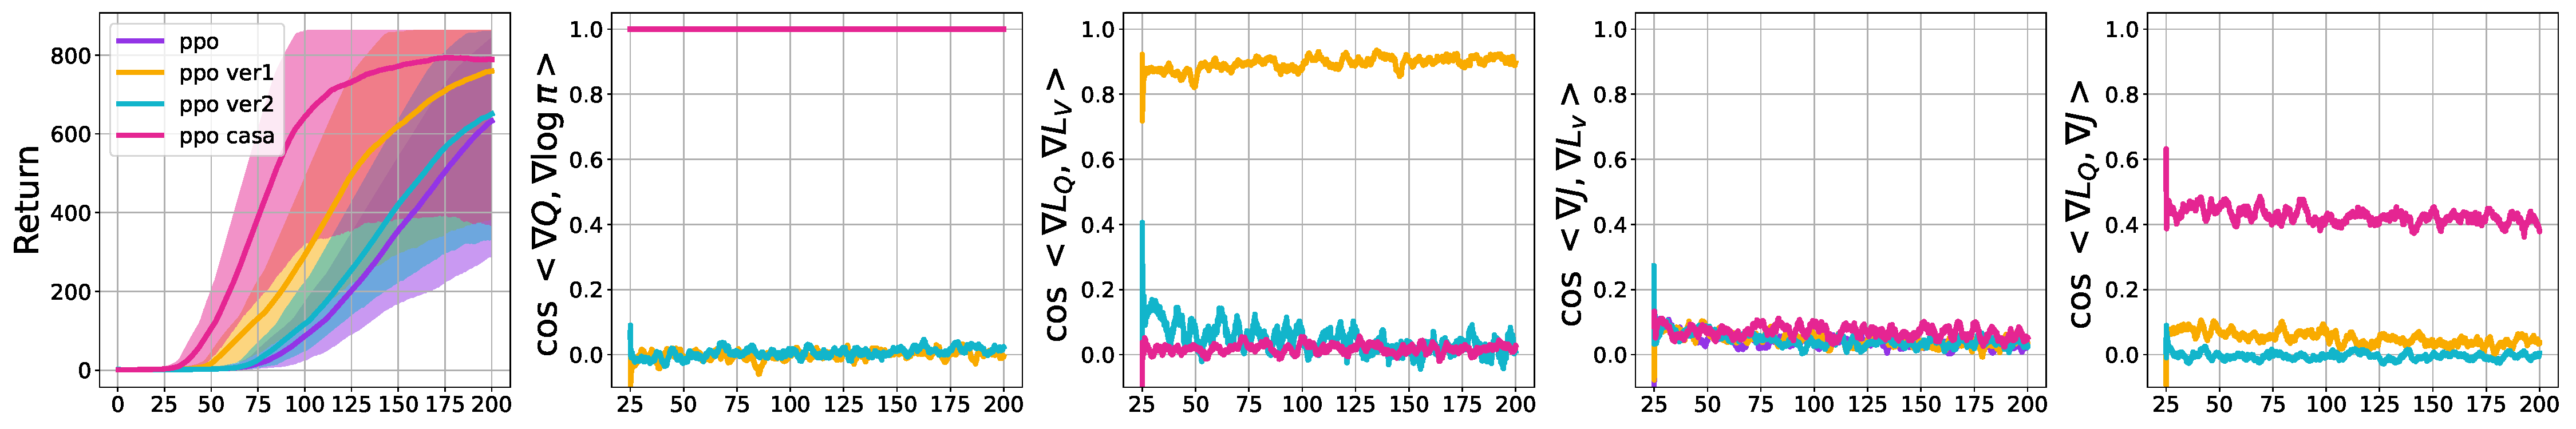
\includegraphics[width=\linewidth]{body/app_fig/app_ppo_Breakout.pdf}

% 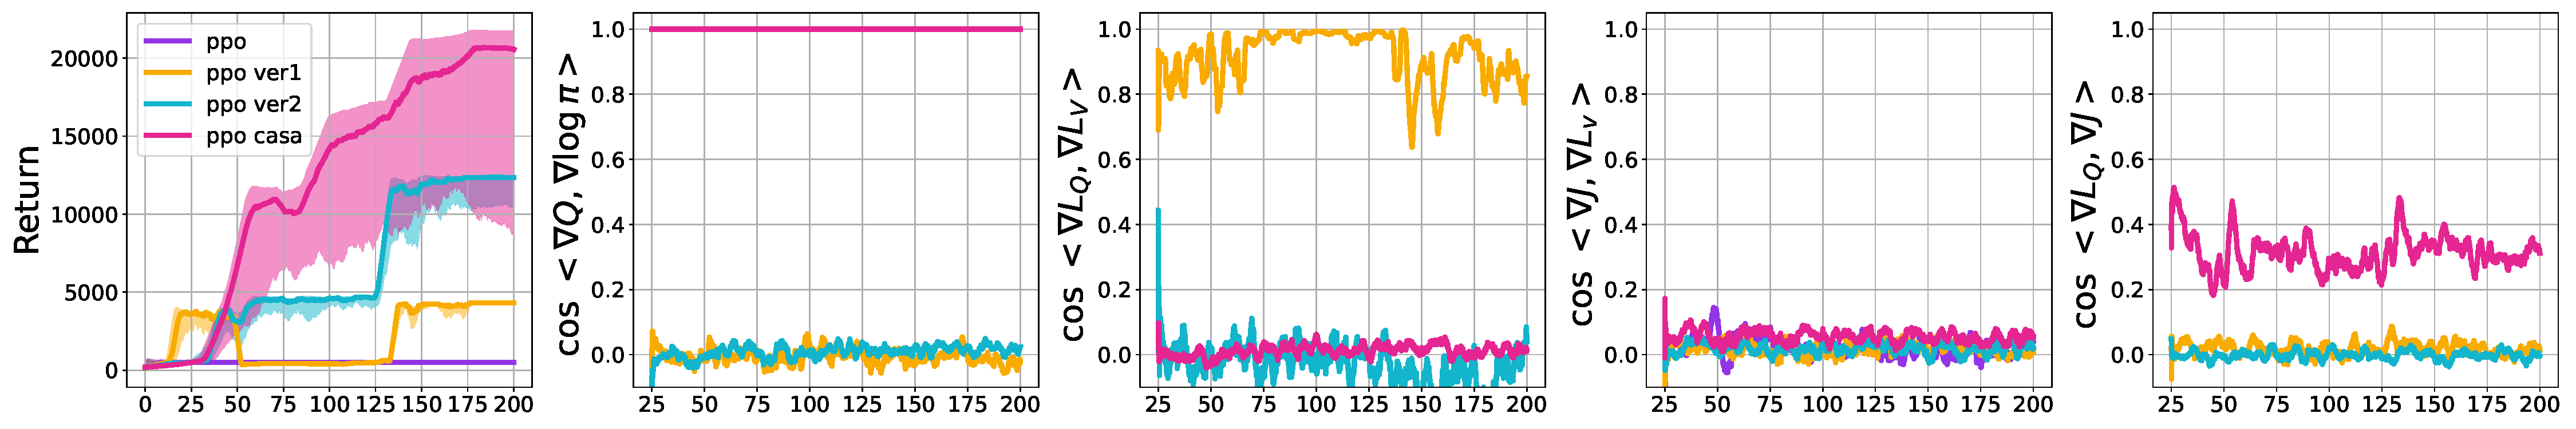
\includegraphics[width=\linewidth]{body/app_fig/app_ppo_Qbert.pdf}

% 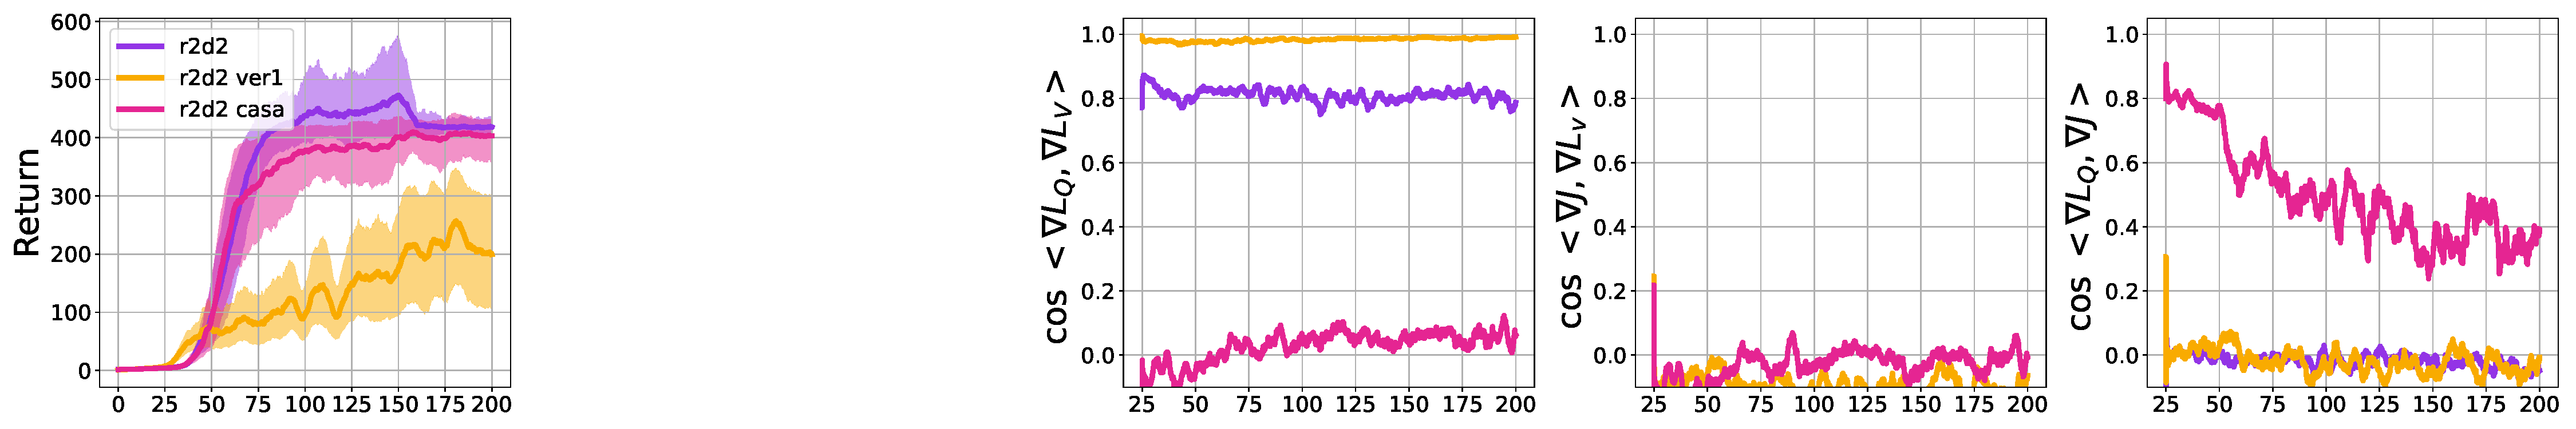
\includegraphics[width=\linewidth]{body/app_fig/app_r2d2_Breakout.pdf}


% 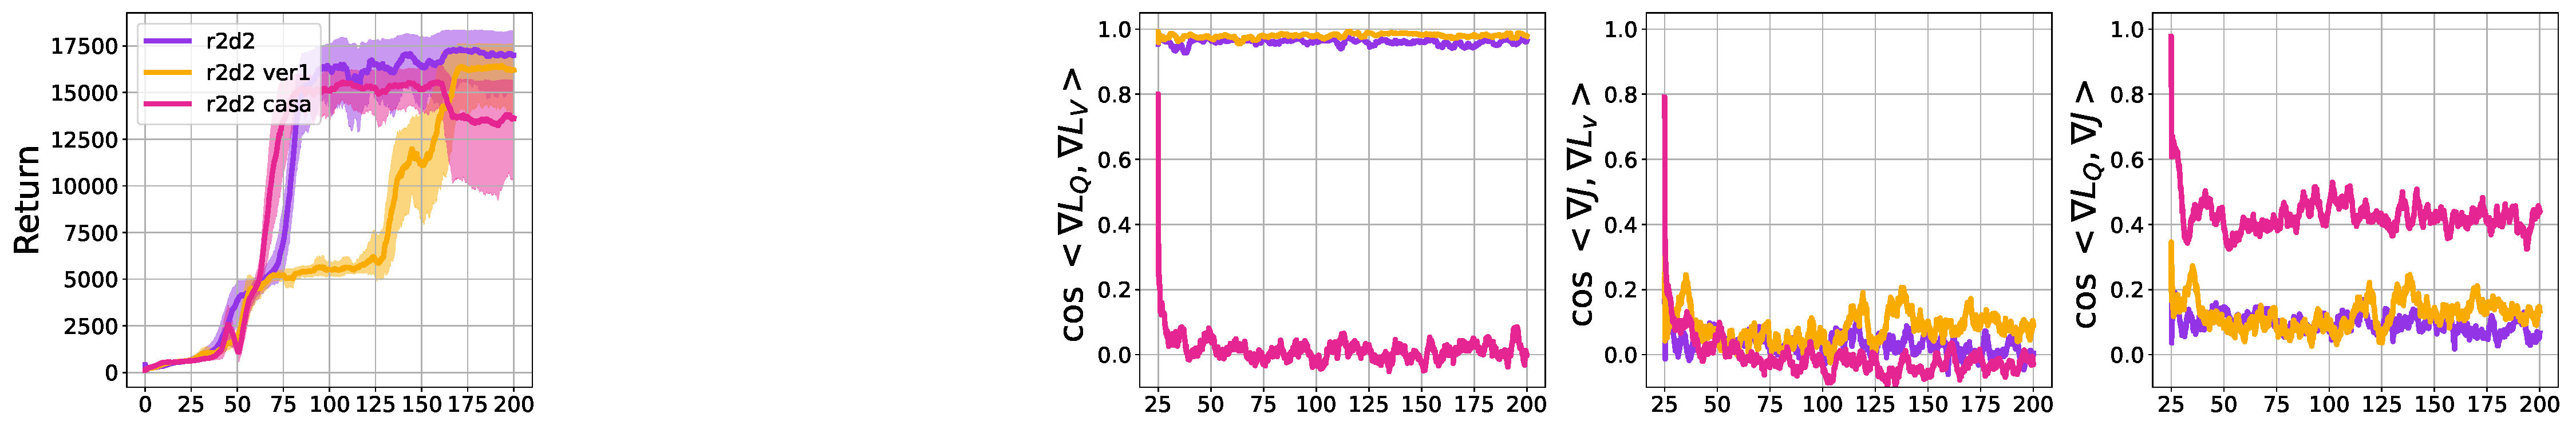
\includegraphics[width=\linewidth]{body/app_fig/app_r2d2_Qbert.pdf}
% \caption{Angles of Gradients and Returns of versions of PPO and R2D2 defined in Table \ref{tab:ppo_mtv} and Table \ref{tab:r2d2_mtv}.}
% \label{fig:mtv_app}
% \end{figure}

% \clearpage

% \changnan{casa summary deleted}
% \section{CASA summary}
% \begin{figure}[ht]
% \centering
% 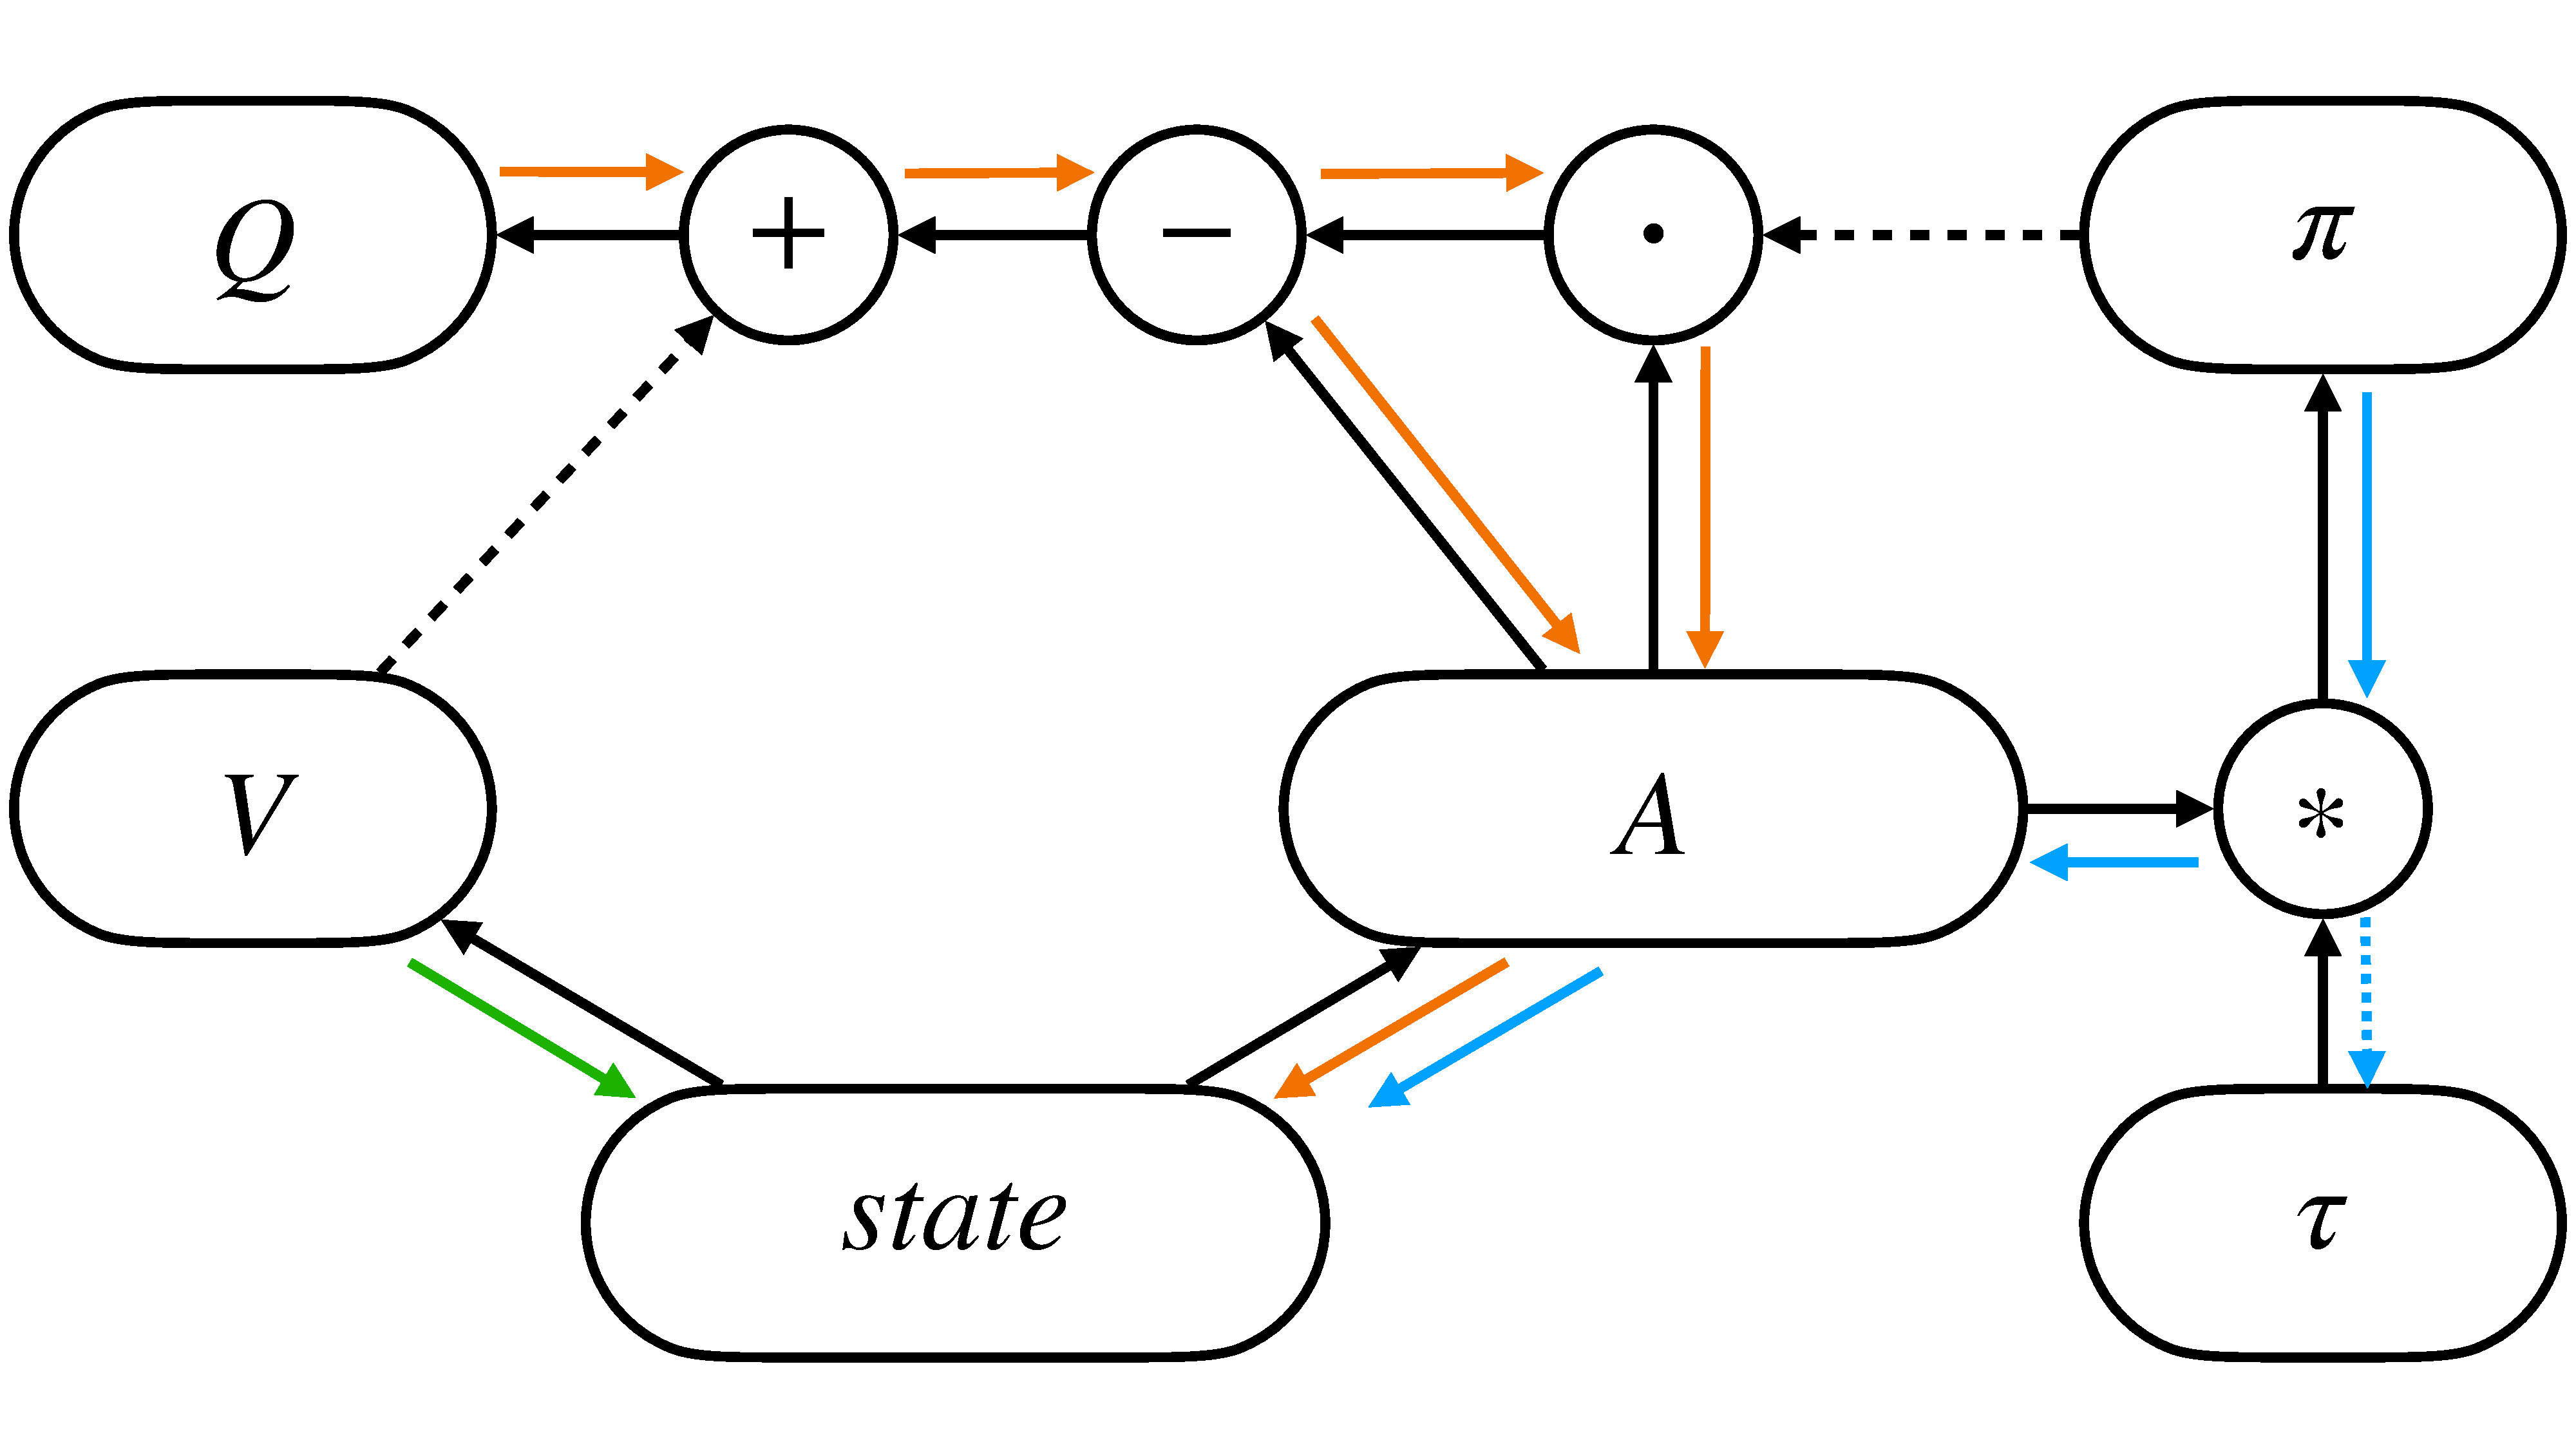
\includegraphics[width=0.4\textwidth,bb= 0 0 1800 1100]{body/figures/CASA.pdf}
% \caption{
% \textbf{Black} lines represent the forward process.
% \textbf{Dotted} black lines represent the \textit{stop gradient} operator in the forward process. 
% \textbf{Colorful} lines represent backpropagation from different loss functions. 
% Specifically, \textbf{blue} lines represent $\mathbb{E}_\pi [(Q^\pi-V)\nabla \log \pi]$, 
% \textbf{orange} lines represent $\mathbb{E}_\pi [(Q^\pi-Q)\nabla Q]$,
% and \textbf{green} lines represent $\mathbb{E}_\pi [(Q^\pi-V)\nabla V]$.}
% \label{fig:casa}
% \end{figure}
% \section{motivation experiments}

\clearpage

{\colorred \section{On Discussing Application of CASA on Continuous Action Space}
\label{app:cts_space}

As we can see CASA is only applied to discrete action space in the main context, we make a discussion on whether CASA is applicable on continuous action space. 
For brevity, we let $\tau=1$ and write \eqref{eq:casa} as:
\begin{equation}
\left\{
    \begin{aligned}
        &\pi = \text{softmax}(A), \\
        &\Bar{A} = A - \mathbb{E}_{\pi} [A], \\
        &Q = \Bar{A} + sg(V).
    \end{aligned}
\right. 
\end{equation}
The difficulty comes from estimating two quantities, one is $\text{softmax}(A)$, the other is $\mathbb{E}_{\pi} [A]$. 
This comes from the fact that discrete action space is countable so these two quantities are expressed in a closed-form, while continuous action space is uncountable so an accurate estimation of these two quantities is intractable. 
We can surely apply Monte Carlo methods to approximate, but a more elegant close-form expression may be preferred. 
Then this becomes another problem: \textit{how to estimate (state-action values / advantages / policy probabilities) of all actions in a continuous action space efficiently without loss of generality?}
This is another representational design problem, which is out of scope of this paper, so we don't touch much about it. 
But with the hope of inspiring a better solution to this problem, we provide one practical way of applying CASA on continuous action space based on kernel-based machine learning. 

Let $a_0, \dots, a_k$ to be basis actions in the action space. 
Let $A(s, a_0), \dots, A(s, a_k)$ to be advantage functions for tuples of states and basis actions. 
They can either share parameters or be isolated. 
Let $K(\cdot, \cdot)$ be a kernel function defined on the product of two action spaces. 
For any $a$ in the action space, we can estimate $A(s, a)$ by a decomposition such like $$A(s, a) = \frac{1}{Z_a} (K(a_0, a) A(s, a_0) + \dots + K(a_k, a) A(s, a_k)),$$ where $Z_a = \sum_{i=0}^k K(a_i, a)$ is a normalization constant. 

Since $K(\cdot, a)$ is a closed-form function of $a$, and $|\{A(s, a_0), \dots, A(s, a_k)\}|$ is finite, we can make a closed-form expression of both $\text{softmax}(A)$ and $\mathbb{E}_{\pi} [A]$. 
Then we can apply CASA directly on this expression, with one function estimates $V$ and the other function estimates advantages of all actions in a closed-form with only state as input.  
The policy is defined directly by $\text{softmax}$ of all advantages. 
In details, we define
\begin{equation}
\left\{
    \begin{aligned}
        &\pi(s, a) = \exp (A(s, a)) / \int_{a} \exp (A(s, a)) da, \\
        &\Bar{A}(s, a) = A(s, a) - \int_{a} sg(\pi(s, a)) A(s, a) da, \\
        &Q(s, a) = \Bar{A}(s, a) + sg(V(s)).
    \end{aligned}
\right. 
\end{equation}

Then it satisfies the consistency of CASA on continuous action space.
$$
\begin{aligned}
    \nabla \log \pi(s, a) &= \nabla A(s, a) - \frac{\nabla \int_{a} \exp (A(s, a)) da}{\int_{a} \exp (A(s, a)) da} \\
    &= \nabla A(s, a) - \frac{ \int_{a} \exp (A(s, a)) \nabla A(s, a) da}{\int_{a} \exp (A(s, a)) da} \\
    &= \nabla A(s, a) - \int_{a} \frac{  \exp (A(s, a)) }{\int_{a} \exp (A(s, a)) da} \nabla A(s, a) da \\
    &= \nabla A(s, a) - \int_{a} \pi(s, a) \nabla A(s, a) da \\
    &= \nabla \Bar{A}(s, a) = \nabla Q(s, a). 
\end{aligned}
$$
}

\section{DR-Trace}
\label{app:drtrace}

% One simple choice is to learn $V$ and $\pi$ by V-Trace \citep{impala} and to learn $Q$ by ReTrace \citep{retrace}. 
% \citep{impala} shows that $V^{\Tilde{\pi}}$ estimated by V-Trace converges to $V^*$ that corresponds to some $\Tilde{\pi}_{VTrace}$.
% Respectively, \citep{retrace} shows that $Q^{\Tilde{\pi}}$ estimated by ReTrace converges to $Q^*$ that corresponds to some $\Tilde{\pi}_{ReTrace}$.

As CASA estimates $(V, Q, \pi)$, we would ask
\textbf{i)} how to guarantee that $\Tilde{\pi}_{VTrace} = \Tilde{\pi}_{ReTrace}$, 
\textbf{ii)} how to exploit $(V, Q, \pi)$ to make a better estimation. 
Though we can apply V-Trace to estimate $V$ and ReTrace to estimate $Q$ with proper hyperparameters to guarantee $\Tilde{\pi}_{VTrace} = \Tilde{\pi}_{ReTrace}$, it's more reasonable to estimate $(V, Q)$ together. 
Inspired by Doubly Robust, which is shown to maximally reduce the variance, we introduce DR-Trace, which estimates $V$ by 
$$
\label{eq:dr-v}
    \begin{aligned}
        V_{DR}^{\Tilde{\pi}} (s_t) &\overset{def}{=} \mathbb{E}_{\mu} [ 
        V(s_t) + \sum_{k \geq 0} \gamma^k 
     c_{[t:t+k-1]} \rho_{t+k}  \delta^{DR}_{t+k} ],  
    \end{aligned}
$$
{\colorred where $\mu$ is the behavior policy}, $\delta^{DR}_t \overset{def}{=} r_t + \gamma V(s_{t+1}) - Q(s_t, a_t)$ is one-step Doubly Robust error, $\rho_t \overset{def}{=} \min\{\frac{\pi_t}{\mu_t}, \Bar{\rho} \}$ and $c_t \overset{def}{=} \min\{\frac{\pi_t}{\mu_t}, \Bar{c}\}$ are clipped per-step importance sampling, $c_{[t: t+k]} \overset{def}{=} \prod_{i=0}^{k} c_{t+i}$.

With one step Bellman equation, we estimate $Q$ by
$$
\label{eq:dr-q}
    \begin{aligned}
         Q_{DR}^{\Tilde{\pi}} (s_t, a_t) 
         &\overset{def}{=} \mathbb{E}_{s_{t+1}, r_t \sim p(\cdot, \cdot | s_t, a_t)} [  r_t + \gamma   V_{DR}^{\Tilde{\pi}} (s_{t+1}) ] 
        \\
        %  &=  \mathbb{E}_{\mu} [ r_t + \gamma V(s_{t + 1}) +
        % \gamma \sum_{k \geq 0} \gamma^k 
        % c_{[t+1:t+k]} \rho_{t+1+k}
        % \delta^{DR}_{t+1+k} V
        % ]
        % \\
        %  &= \mathbb{E}_{\mu}   [
        % Q(s_t, a_t) + \delta_t^{DR}V + \sum_{k \geq 1}  \gamma^k
        % c_{[t+1:t+k-1]} \rho_{t+k}
        % \delta^{DR}_{t+k} V
        % ],
        % \\
        &=  \mathbb{E}_{\mu}   [
        Q(s_t, a_t) + \sum_{k \geq 0}  \gamma^k
        c_{[t+1:t+k-1]} \Tilde{\rho}_{t, k}
        \delta^{DR}_{t+k}
        ], 
    \end{aligned}
$$
where $\Tilde{\rho}_{t, k} =  1_{\{k=0\}} + 1_{\{k > 0\}} \rho_{t+k}$.

% Compared to \eqref{eq:dr-v}, $c_{[t+1:t+k-1]} \Tilde{\rho}_{t, k}$ in \eqref{eq:dr-q} doesn't multiply importance sampling ratio of $a_t$, which meets the same intuition as \eqref{eq:vtrace} and \eqref{eq:retrace}.\\
\begin{theorem}
    Define $\Bar{A} = A - \mathbb{E}_\pi[A]$, $Q = \Bar{A} + sg(V)$,
    $$
    \begin{aligned}
    &\mathscr{T}(Q) \overset{def}{=} \mathbb{E}_{\mu}   [
        Q(s_t, a_t) + \sum_{k \geq 0}  \gamma^k
        c_{[t+1:t+k-1]} \Tilde{\rho}_{t, k}
        \delta^{DR}_{t+k}
        ], \\
    &\mathscr{S}(V) \overset{def}{=} \mathbb{E}_{\mu}   [
        V(s_t) + \sum_{k \geq 0}  \gamma^k
        c_{[t:t+k-1]} \rho_{t, k}
        \delta^{DR}_{t+k}
        ], \\
    &\mathscr{U}(Q, V) = (\mathscr{T}(Q) - \mathbb{E}_\pi[Q] + \mathscr{S}(V), \mathscr{S}(V)), \\
    &\mathscr{U}^{(n)}(Q, V) = \mathscr{U}(\mathscr{U}^{(n-1)}(Q, V)),
    \end{aligned}
    $$
    then $\mathscr{U}^{(n)}(Q, V) \rightarrow (Q^{\Tilde{\pi}}, V^{\Tilde{\pi}})$ that corresponds to 
    $$
        \Tilde{\pi}(a|s) = \frac
        {\min \left\{\Bar{\rho} \mu (a|s), \pi(a|s)\right\}}
        {\sum_{b \in \mathcal{A}}\min \left\{\Bar{\rho} \mu (b|s), \pi(b|s)\right\}}.
    $$ as $n \rightarrow +\infty$.
\label{thm:dr}
\end{theorem}
\begin{proof}
    See Appendix \ref{app:proof}, Theorem \ref{thm_app:dr}.
\end{proof}
Theorem \ref{thm:dr} shows that DR-Trace is a contraction mapping and $(V, Q)$ converges to $(V^{\Tilde{\pi}}, Q^{\Tilde{\pi}})$ that corresponds to 
$$
    \begin{aligned}
        \Tilde{\pi}(a|s) = \frac
        {\min \left\{\Bar{\rho} \mu (a|s), \pi(a|s)\right\}}
        {\sum_{b \in \mathcal{A}}\min \left\{\Bar{\rho} \mu (b|s), \pi(b|s)\right\}}.
    \end{aligned}
$$

% At training time, the policy evaluation is achieved by updating $\theta$ to minimize $l2$ losses
% $$
% \begin{aligned}
%     L_V(\theta) &= \mathbb{E}_\pi [ (V_\theta(s_t) -  V_{DR}^{\Tilde{\pi}} (s_t))^2 ], \\
%     L_Q(\theta) &= \mathbb{E}_\pi [ (Q_\theta(s_t, a_t) -  Q_{DR}^{\Tilde{\pi}} (s_t, a_t))^2 ],
% \end{aligned}
% $$ 
% which gives the ascent direction of $\theta$ by
% \begin{equation}
% \label{eq:grad_qv}
%     \begin{aligned}
%         \nabla_\theta L_V(\theta)
%         &= \mathbb{E}_\pi \left[ (V_{DR}^{\Tilde{\pi}} (s_t) - V_\theta(s_t) ) \nabla V_\theta(s_t) \right], \\
%         \nabla_\theta L_Q(\theta)
%         &= \mathbb{E}_\pi \left[ (Q_{DR}^{\Tilde{\pi}} (s_t, a_t) - Q_\theta(s_t, a_t)) \nabla Q_\theta(s_t, a_t) \right].
%     \end{aligned}
% \end{equation}
% And we make the policy improvement by policy gradient, which gives the ascent direction of $\theta$ by 
% \begin{equation}
% \label{eq:grad_pi}
% \begin{aligned}
%     \nabla_\theta \mathcal{J}(\tau, \theta) = \mathbb{E}_\mu \left[\tau \rho_t (Q_{DR}^{\Tilde{\pi}} (s_t, a_t) - V_\theta(s_t) ) \nabla_\theta \log \pi_t \right],
% \end{aligned}
% \end{equation}
% where $\mathcal{J} (\tau, \theta) = \tau \mathbb{E}_\pi [\sum \gamma^t r_t]$.
% It takes an additional $\tau$, which frees the scale of gradient from $\tau$.

% Finally, the gradient ascent direction of $\theta$ is given by
% \begin{equation}
%     \label{eq:grad_all}
%     \alpha_1 \nabla_\theta L_V + \alpha_2 \nabla_\theta L_Q + \alpha_3 \nabla_\theta \mathcal{J}.
% \end{equation}

% \textbf{Full algorithm is described in Appendix \ref{app:casa}.}
% Note that \eqref{eq:grad_all} doesn't need any entropy regularization. 
% We will discuss why this happens in section \ref{sec:equiv} and how CASA controls the exploration in section \ref{sec:ent_control}.


\begin{figure}[h]
    \centering
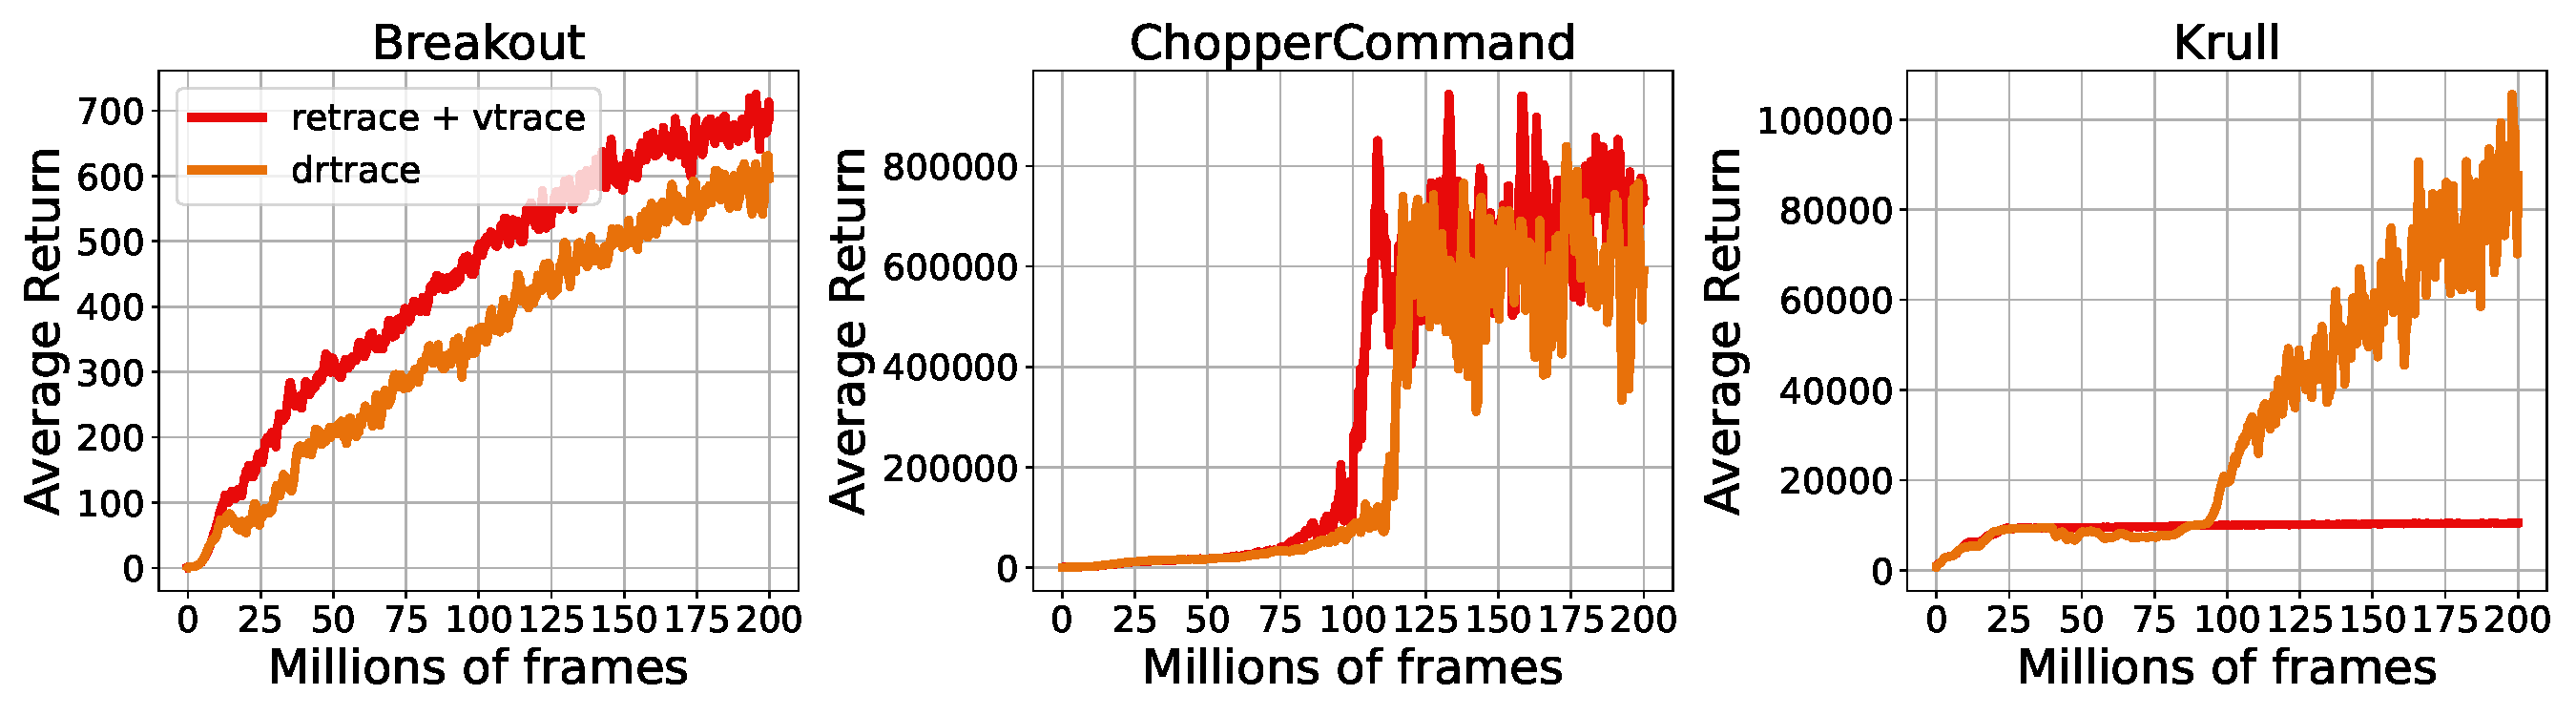
\includegraphics[width=\linewidth]{body/ablation/dr_ablation.pdf}
    \caption{Ablation study for w/wo DR-Trace on Breakout, ChopperCommand and Krull.}
    \label{fig:app_dr_trace}
\end{figure}

According to our proof, DR-Trace should work similar to V-Trace and ReTrace, as the convergence rate and the limitation are same. 
We compare DR-Trace with V-Trace+ReTrace in Figure \ref{fig:app_dr_trace}, where we replace estimation of state values by V-Trace and estimation of state-action values by ReTrace. 
We call V-Trace+ReTrace as No-DR-Trace for brevity. 
No-DR-Trace performs better on Breakout and ChopperCommand, but fails to make a breakthrough on Krull. 
Recalling the fact that Doubly Robust can maximally reduce the variance of Bellman error, No-DR-Trace is less stable but also potential to achieve a better performance. 
A conclusion cannot be made about No-DR-Trace, as this phenomenon means that No-DR-Trace is less stable than DR-Trace, but it also holds the potential to achieve a better performance.

% \clearpage


\section{Proofs}
\label{app:proof}

\theoremstyle{plain}
% \setcounter{Lemma}{0}
\newtheorem{Lemma_app}{Lemma}[section]
\newtheorem{Theorem_app}{Theorem}[section]
\theoremstyle{definition}
\newtheorem*{Remark_app}{Remark}
\theoremstyle{remark}

% \begin{Lemma_app}
% Let 
% $g \in \textbf{C}^{1}(\mathbb{R}^{n}): \mathbb{R}^{n} \to \mathbb{R}^{n}, \ f \in \textbf{C}^{1}(\mathbb{R}^{n+k}): \mathbb{R}^{n+k} \to \mathbb{R}^{n}.
% $\\
% If
% $
% \nabla_x g(x) = \nabla_x f(x, y)$, for $\forall x\in \mathbb{R}^{n}, y\in \mathbb{R}^k,
% $
% then $\exists$ $c \in \textbf{C}^{1}(\mathbb{R}^{k}): \mathbb{R}^{k} \to \mathbb{R}^{n}$, s.t. $f(x, y) = g(x) + c(y)$.
% \label{lemma_app:func_sep}
% \end{Lemma_app}
% \begin{proof}

% Let $\Tilde{f}(x, y) = f(x, y) - g(x)$.

% Since $\nabla_x g(x) = \nabla_x f(x, y)$, we have 
% $$
% \nabla_x \Tilde{f} = 0, \ for \ \forall x\in \mathbb{R}^{n}, y\in \mathbb{R}^k.
% $$

% So $\Tilde{f}$ is a constant function w.r.t $x$, which can be denoted as $c(y) = \Tilde{f}(x, y)$.

% Hence, $f(x, y) = g(x) + c(y)$.
% \end{proof}

\begin{Lemma_app}
(i) Define $\pi = softmax(A / \tau)$, then $\nabla \log \pi = (\textbf{1} - \pi) \frac{\nabla A}{\tau}$. 
(ii) Denote $sg$ to be stop gradient and define $\Bar{A} = A - \mathbb{E}_\pi [A]$, $Q = \Bar{A} + sg(V)$, then $\nabla Q = (\textbf{1} - \pi) \nabla A$.
\label{lemma_app:vannila_grad}
\end{Lemma_app}
\begin{proof}

As $Q = \Bar{A} + sg(V) = A - sg(\pi)\cdot A + sg(V)$, it's obvious that $\nabla Q = (\textbf{1} - \pi) \nabla A$.

For $\log \pi$, it's a standard derivative of cross entropy, so we have $\nabla \log \pi = (\textbf{1} - \pi) \nabla (A / \tau) = (\textbf{1} - \pi) \frac{\nabla A}{\tau}$.
\end{proof}

\begin{Lemma_app}
Define $\Bar{A}= A - \mathbb{E}_\pi[A]$, $Q = \Bar{A} + sg(V), \pi = softmax(A / \tau)$, then 
$$
\mathbb{E}_\pi \left[ (Q - V) \nabla \log \pi \right]
= - \tau \nabla \textbf{H}[\pi].
$$
\label{lemma_app:eqiv_pg_ent}
\end{Lemma_app}
\begin{proof}
Since 
$$
\pi = \exp(A / \tau) / Z,\ Z = \int_\mathcal{A} \exp(A / \tau),
$$
we have 
$$
A = \tau \log \pi + \tau \log Z.
$$
Based on the observation that $\mathbb{E}_\pi \left[ f(s) \nabla \log \pi (\cdot | s) \right] = 0$, 
we have 
$$\mathbb{E}_\pi \left[ \mathbb{E}_\pi[A] \cdot \nabla \log \pi \right] = 0,$$ 
$$\mathbb{E}_\pi \left[ \log Z \cdot \nabla \log \pi \right] = 0.$$

On the one hand,
$$
\begin{aligned}
    \mathbb{E}_\pi \left[ (Q - V) \nabla \log \pi \right]
    &= \mathbb{E}_\pi \left[ A \nabla \log \pi \right] 
    - \mathbb{E}_\pi \left[ \mathbb{E}_\pi[A] \cdot \nabla \log \pi \right] \\
    &= \tau \mathbb{E}_\pi \left[ \log \pi \nabla \log \pi \right]
    + \tau \mathbb{E}_\pi \left[ \log Z \cdot \nabla \log \pi \right] \\
    &= \tau \mathbb{E}_\pi \left[ \log \pi \nabla \log \pi \right].
\end{aligned}
$$

On the other hand, 
$$
\begin{aligned}
    \nabla \textbf{H} [\pi] 
    &= - \nabla \int_\mathcal{A} \pi_i \log \pi_i \\
    &= - \int_\mathcal{A}  \nabla \pi_i \cdot \log \pi_i - \int_\mathcal{A} \pi_i \nabla \log \pi_i  \\
    &= - \int_\mathcal{A}  \pi_i \nabla \log \pi_i \cdot \log \pi_i - \int_\mathcal{A}  \pi_i \frac{\nabla \pi_i}{\pi_i} \\
    &= - \mathbb{E}_\pi \left[ \log \pi \nabla \log \pi \right].
\end{aligned}
$$
Hence, $
\mathbb{E}_\pi \left[ (Q - V) \nabla \log \pi \right]
= - \tau \nabla \textbf{H}[\pi]
$.
\end{proof}

\begin{Theorem_app}
    Define $\Bar{A} = A - \mathbb{E}_\pi[A]$, $Q = \Bar{A} + sg(V)$.
    Define $$
    \begin{aligned}
    &\mathscr{T}(Q) \overset{def}{=} \mathbb{E}_{\mu}   [
        Q(s_t, a_t) + \sum_{k \geq 0}  \gamma^k
        c_{[t+1:t+k-1]} \Tilde{\rho}_{t, k}
        \delta^{DR}_{t+k}
        ], \\
    &\mathscr{S}(V) \overset{def}{=} \mathbb{E}_{\mu}   [
        V(s_t) + \sum_{k \geq 0}  \gamma^k
        c_{[t:t+k-1]} \rho_{t, k}
        \delta^{DR}_{t+k}
        ], \\
    &\mathscr{U}(Q, V) = (\mathscr{T}(Q) - \mathbb{E}_\pi[Q] + \mathscr{S}(V), \mathscr{S}(V)), \\
    &\mathscr{U}^{(n)}(Q, V) = \mathscr{U}(\mathscr{U}^{(n-1)}(Q, V)),
    \end{aligned}
    $$
    then $\mathscr{U}^{(n)}(Q, V) \rightarrow (Q^{\Tilde{\pi}}, V^{\Tilde{\pi}})$ that corresponds to 
    $$
        \Tilde{\pi}(a|s) = \frac
        {\min \left\{\Bar{\rho} \mu (a|s), \pi(a|s)\right\}}
        {\sum_{b \in \mathcal{A}}\min \left\{\Bar{\rho} \mu (b|s), \pi(b|s)\right\}}.
    $$ as $n \rightarrow +\infty$.
\label{thm_app:dr}
\end{Theorem_app}
\begin{Remark_app}
$\mathscr{T}(Q) - \mathbb{E}_\pi[Q] + \mathscr{S}(V)$ is \textbf{exactly} how $Q$ is updated at training time. 
Since $Q = \Bar{A} + sg(V)$, if we apply gradient ascent on $Q$ and $V$ in directions $\nabla L_Q(\theta)$ and $\nabla L_V(\theta)$ respectively, change of $Q$ comes from two aspects. One comes from $\nabla L_Q(\theta)$, which changes $A$, the other comes from $\nabla L_V(\theta)$, which changes $V$. Because the gradient of $V$ is stopped when estimating $Q$, the latter is captured by "minus old baseline, add new baseline", which is $- \mathbb{E}_\pi[Q] + \mathscr{S}(V)$ in Theorem \ref{thm_app:dr}.
\end{Remark_app}
\begin{proof}
 Define
 $$
 \begin{aligned}
        \widetilde{\mathscr{T}}(Q) &= - \mathbb{E}_\pi[Q] + \mathscr{T}(Q), \\
        \widetilde{\mathscr{U}}(Q, V) &= (\widetilde{\mathscr{T}}(Q), \mathscr{S}(V)), \\
        \widetilde{\mathscr{U}}^{(n)}(Q, V) &=   \widetilde{\mathscr{U}}(\widetilde{\mathscr{U}}^{(n-1)}(Q, V)).
 \end{aligned}
 $$
By Lemma \ref{lemma_app:dr_q}, $\widetilde{\mathscr{T}}^{(n)}(Q)$ converges to some $A^*$ as $n \rightarrow \infty$. This process will not influence the estimation of $V$ as the gradient of $V$ is stopped when estimating $Q$. According to the proof, $A^*$ does not depend on $V$. \\
By Lemma \ref{lemma_app:dr_v}, $\mathscr{S}^{(n)}(V)$ converges to some $V^*$ as $n \rightarrow \infty$. \\
Hence, we have
$$
\widetilde{\mathscr{U}}^{(n)}(Q, V) \rightarrow (A^*, V^*)\ \ as\ \ n \rightarrow +\infty. 
$$
By definition, 
$$
\mathscr{U}(Q, V) = (\widetilde{\mathscr{T}}(Q) + \mathscr{S}(V), \mathscr{S}(V)),
$$
we can regard $\widetilde{\mathscr{T}}(Q) + \mathscr{S}(V)$ as $Q$ and regard $\mathscr{S}(V)$ as $V$, then
$$
\begin{aligned}
    \mathscr{U}^{(2)}(Q, V) 
    &= \mathscr{U}(\widetilde{\mathscr{T}}(Q) + \mathscr{S}(V), \mathscr{S}(V)) \\
    &= (\mathscr{T}(\widetilde{\mathscr{T}}(Q) + \mathscr{S}(V)) -\mathscr{S}(V) + \mathscr{S}^{(2)}(V), \mathscr{S}^{(2)}(V)) \\
    &= (\widetilde{\mathscr{T}}^{(2)}(Q) + \mathscr{S}^{(2)}(V), \mathscr{S}^{(2)}(V)).
\end{aligned}
$$
By induction, 
$$
\begin{aligned}
    \mathscr{U}^{(n)}(Q, V) &= (\widetilde{\mathscr{T}}^{(n)}(Q) + \mathscr{S}^{(n)}(V), \mathscr{S}^{(n)}(V)) \\
    &\rightarrow (A^*+V^*, V^*)\ \ as\ \ n\rightarrow + \infty.
\end{aligned}
$$
Same as \citep{impala}, 
$$
    \Tilde{\pi}(a|s) = \frac
    {\min \left\{\Bar{\rho} \mu (a|s), \pi(a|s)\right\}}
    {\sum_{b \in \mathcal{A}}\min \left\{\Bar{\rho} \mu (b|s), \pi(b|s)\right\}}.
$$ 
is the policy s.t. the Bellman equation holds, which is 
$$\mathbb{E}_\mu[\rho_t (r_t + \gamma V_{t+1} - V_t) | \mathscr{F}_t] = 0,$$ and $\mathscr{U}(Q^{\Tilde{\pi}}, V^{\Tilde{\pi}}) = (Q^{\Tilde{\pi}}, V^{\Tilde{\pi}})$. \\
So we have
$(A^*+V^*, V^*) = (Q^{\Tilde{\pi}}, V^{\Tilde{\pi}}).$
\end{proof}

\begin{Lemma_app}
Define $\Bar{A}= A - \mathbb{E}_\pi[A]$, $Q = \Bar{A} + sg(V)$,
then operator 
$$
    \mathscr{T}(Q) \overset{def}{=} \mathbb{E}_{\mu}   [
        Q(s_t, a_t) + \sum_{k \geq 0}  \gamma^k
        c_{[t+1:t+k-1]} \Tilde{\rho}_{t, k}
        \delta^{DR}_{t+k}
        ]
$$
is a contraction mapping w.r.t. $Q$.
\label{lemma_app:dr_q}
\end{Lemma_app}
\begin{Remark_app}
Note that $\mathscr{T}(Q)$ is exactly \eqref{eq:dr-q}. 

Since $Q = A + sg(V)$, the gradient of $V$ is stopped when estimating $Q$, updating $Q$ will not change $V$, which is equivalent to updating $A$.
Without loss of generality, we assume $V$ is fixed as $V^*$ in the proof.
\end{Remark_app}
\begin{proof}

$\Bar{A} = A - \mathbb{E}_\pi[A]$ shows $\mathbb{E}_\pi[\Bar{A}] = 0$, which guarantees that no matter how we update $A$, we always have $\mathbb{E}_\pi[Q] = V^*$.

Based on above observations, define 
$$
    \widetilde{\mathscr{T}}(Q) \overset{def}{=} - \mathbb{E}_\pi [Q] + \mathscr{T}(Q).
$$

It's obvious that we only need to prove $\widetilde{\mathscr{T}}(Q)$ is a contraction mapping.

For brevity, we denote $$Q_t = Q(s_t, a_t), A_t = A(s_t, a_t), V^*_t = V^*(s_t).$$

Noticing that $\Tilde{\rho}_{t, 0} = 1$, let $\mathscr{F}$ represent filtration, we can rewrite $\widetilde{\mathscr{T}}$ as 
\begin{equation}
\label{eq:dr_a_2}
\begin{aligned}
    \widetilde{\mathscr{T}}(Q)
    &= \mathbb{E}_{\mu}   [
        A_t + \sum_{k \geq 0}  \gamma^k
        c_{[t+1:t+k-1]} \Tilde{\rho}_{t, k}
        \delta^{DR}_{t+k}
        ] \\
    &= \mathbb{E}_{\mu}   [
        -V^*_t + \sum_{k \geq 0}  \gamma^k
        c_{[t+1:t+k-1]} \Tilde{\rho}_{t, k}
        r_{t+k}
        + 
        \sum_{k \geq 0}  \gamma^{k+1}
        c_{[t+1:t+k-1]} \Delta_k ],
        \\
\end{aligned}
\end{equation}
where 
\begin{equation}
\label{eq:dr_delta}
    \Delta_k = \mathbb{E}_{\mu}\left[\Tilde{\rho}_{t, k} V^*_{t+k+1} - c_{t+k} \Tilde{\rho}_{t, k+1} Q_{t+k+1} | \mathscr{F}_{t+k}\right].
\end{equation}
By definition of $Q$,
$$
    \mathbb{E}_{\mu}[V_{t+k+1}^*|\mathscr{F}_{t+k}] 
    = \mathbb{E}_{\mu}[
    \mathbb{E}_\pi[Q_{t+k+1}|\mathscr{F}_{t+k+1}]
    |\mathscr{F}_{t+k}], \\
    % \geq&  \mathbb{E}_{\mu}[
    % \mathbb{E}_\mu[\Tilde{\rho}_{t, k+1} Q_{t+k+1}|\mathscr{F}_{t+k+1}]
    % |\mathscr{F}_{t+k}], 
$$
we can rewrite \eqref{eq:dr_delta} as
\begin{equation}
\label{eq:dr_q_delta}
\Delta_k = \mathbb{E}_{\mu}[
(
\Tilde{\rho}_{t, k} \frac{\pi_{t+k+1}}{\mu_{t+k+1}}- c_{t+k} \Tilde{\rho}_{t, k+1} 
) Q_{t+k+1} | \mathscr{F}_{t+k}
].
\end{equation}
For any $Q_1 = A_1 + sg(V^*)$, $Q_2 = A_2 + sg(V^*)$, since
$$
\mathbb{E}_{\mu}[
(
\Tilde{\rho}_{t, k} \frac{\pi_{t+k+1}}{\mu_{t+k+1}}- c_{t+k} \Tilde{\rho}_{t, k+1} 
) | \mathscr{F}_{t+k}
] \geq 0,
$$
by \eqref{eq:dr_a_2} \eqref{eq:dr_q_delta}, we have 
% $$
% || \Delta^1_k - \Delta_k^2 || \leq \mathbb{E}_{\mu}\left[
% \left(
% \Tilde{\rho}_{t, k} \frac{\pi_{t+k+1}}{\mu_{t+k+1}}- c_{t+k} \Tilde{\rho}_{t, k+1} 
% \right) | \mathscr{F}_{t+k}
% \right] ||A^1 - A_2||.
% $$
$$
        || \widetilde{\mathscr{T}}(Q_1) - \widetilde{\mathscr{T}}(Q_2) || 
        % \leq& \mathbb{E}_{\mu} \left[ \sum_{k \geq 0}  \gamma^{k+1} c_{[t+1:t+k-1]} || \Delta_k^1 - \Delta_k^2 || \right] \\
        \leq \mathcal{C} || Q_1 - Q_2 ||,
$$
where 
$$
    \begin{aligned}
        \mathcal{C} 
        &= \mathbb{E}_{\mu} [ \sum_{k \geq 0}  \gamma^{k+1} c_{[t+1:t+k-1]} 
        (
        \Tilde{\rho}_{t, k} \frac{\pi_{t+k+1}}{\mu_{t+k+1}}- c_{t+k} \Tilde{\rho}_{t, k+1} 
        ) ]
        \\
        &= \mathbb{E}_{\mu} [1 -1 + \sum_{k \geq 0}  \gamma^{k+1} c_{[t+1:t+k-1]} 
        \left(
        \Tilde{\rho}_{t, k} - c_{t+k} \Tilde{\rho}_{t, k+1} 
        \right) ] 
        \\
        &= 1 - (1 - \gamma)  \mathbb{E}_{\mu} [\sum_{k \geq 0} \gamma^{k}c_{[t+1:t+k-1]} \Tilde{\rho}_{t, k}  ] \\
        &\leq 1 - (1 - \gamma) < 1.
    \end{aligned}
$$
Hence, $\widetilde{\mathscr{T}}(Q)$ is a contraction mapping and converges to some fixed function, which we denote as $A^*$. So $\mathscr{T}(Q)$ is also a contraction mapping and converges to $A^*+V^*$.
\end{proof}

\begin{Lemma_app}
Define $Q = A + sg(V)$ with $\mathbb{E}_\pi [A] = 0$,
then operator 
$$
    \mathscr{S}(V) \overset{def}{=} \mathbb{E}_{\mu}  [
        V(s_t) + \sum_{k \geq 0}  \gamma^k
        c_{[t:t+k-1]} \rho_{t, k}
        \delta^{DR}_{t+k}
        ]
$$
is a contraction mapping w.r.t. $V$.
\label{lemma_app:dr_v}
\end{Lemma_app}
\begin{Remark_app}
Note that $\mathscr{S}(V)$ is exactly \eqref{eq:dr-v}. 
\end{Remark_app}
\begin{proof}

% Since $Q = A + sg(V)$, updating $V$ wouldn't influence $A$. WLOG, we assume $A$ is fixed as $A^*$ in Lemma \ref{lemma_app:dr_v}. \\
Same as Lemma \ref{lemma_app:dr_q}, we can get
$$
    \Delta_k = \mathbb{E}_{\mu}\left[
    \left( \rho_{t+k} - c_{t+k} \rho_{t+k+1}\right) V_{t+k+1} 
     -  c_{t+k} \rho_{t+k+1} A^*_{t+k+1} | \mathscr{F}_{t+k}\right],
$$
so we have 
$$
    \Delta^1_k - \Delta^2_k = \mathbb{E}_{\mu}\left[ 
    \left( \rho_{t+k} - c_{t+k} \rho_{t+k+1}\right) \cdot  
   (V^1_{t+k+1} -  V^2_{t+k+1})
     | \mathscr{F}_{t+k}\right].
$$
The remaining proof is identical to \citep{impala}'s.
\end{proof}

% \clearpage

% \begin{Lemma_app}
% Let $v \in \mathbb{R}^{|\mathcal{A}|}$ to be a vector. 
% Define 
% $
%     \pi (\tau) = \exp (v / \tau) / Z,\  Z = \int_\mathcal{A}  \exp(v / \tau).
% $
% Let $\Omega$ to be a probability measure supported on $[K, +\infty]$,
% then $f(\Omega) = \mathbb{E}_{\tau \sim \Omega} [\mathbb{E}_{\pi(\tau)} [v]]$ satisfies Lipschitz-1 condition with Wasserstein-1 metric.
% \label{lemma_app:lips}
% \end{Lemma_app}
% \begin{proof}
% Without loss of generality, we assume $v_1 \geq v_2 \geq ... \geq v_{|\mathcal{A}|}$.

% For any $\tau \in [0, +\infty)$, since
% $$
% \begin{aligned}
%     \pi (\tau) = \exp (v / \tau) / Z,\  Z = \int_\mathcal{A}  \exp(v / \tau),
% \end{aligned}
% $$
% we have
% $$
%     v = \tau \log \pi (\tau) + \tau \log Z.
% $$

% Denote $\Tilde{v}_j = v_j / \tau$. \\
% Since 
% $$
% \frac{\partial \log \pi_i}{\partial \Tilde{v}_j} = 1_{i=j} - \pi_j,
% $$
% we have
% $$
% \begin{aligned}
%     \frac{\partial \log \pi_i}{\partial \tau} 
%     &= \sum_j \frac{\partial \log \pi_i}{\partial \Tilde{v}_j} \cdot \frac{\partial \Tilde{v}_j}{\partial \tau} \\
%     &= - \sum_j (1_{i=j} - \pi_j) \frac{v_j}{\tau^2} \\
%     &= - \frac{1}{\tau^2} ( v_i - \sum_j \pi_j v_j ) \\ 
%     &= - \frac{1}{\tau^2} \left( v_i - \mathbb{E}_\pi [v] \right). 
% \end{aligned}
% $$
% Therefore, we have
% $$
% \begin{aligned}
%     \frac{\partial \pi_i}{\partial \tau} 
%     &= \pi_i \frac{\partial \log \pi_i}{\partial \tau} \\
%     &= - \frac{\pi_i}{\tau^2} \left( v_i - \mathbb{E}_\pi [v] \right).
% \end{aligned}
% $$
% Let $f(\tau) = v \cdot \pi(\tau)$, then
% $$
% \frac{\partial f}{\partial \tau} = - \frac{1}{\tau^2} \sum_i v_i \pi_i \left( v_i - \mathbb{E}_\pi [v] \right).
% $$
% Since $\sum_i \mathbb{E}_\pi [v] \pi_i \left( v_i - \mathbb{E}_\pi [v] \right) = 0$,
% we know
% $$
% \begin{aligned}
%     \frac{\partial f}{\partial \tau} 
%     &= - \frac{1}{\tau^2} \sum_i \left( v_i - \mathbb{E}_\pi [v] \right) \pi_i \left( v_i - \mathbb{E}_\pi [v] \right) \\
%     &= - \frac{1}{\tau^2} \sum_i \pi_i \left( v_i - \mathbb{E}_\pi [v] \right)^2 \\
%     &= - \frac{1}{\tau^2} \textbf{Var}_\pi [v].
% \end{aligned}
% $$
% It's obvious that
% $$
% \left| \frac{\partial f}{\partial \tau} \right| \leq \frac{1}{K^2} |v_1 - v_{|\mathcal{A}|}|^2.
% $$
% Hence, for any $\tau_1, \tau_2 \in [K, +\infty]$,
% $$
% |v \cdot \pi(\tau_1) - v \cdot \pi(\tau_2)| \leq C | \tau_1 - \tau_2|.
% $$

% Finally, for any $\gamma \in \Gamma(\Omega_1, \Omega_2)$ \footnote{$\Gamma(\Omega_1, \Omega_2)$ is the collection of all measures on $[K, +\infty] \times [K, +\infty]$ with marginals $(\Omega_1, \Omega_2)$.}, we have
% $$
% \begin{aligned}
% \left| \mathbb{E}_{\tau_1 \sim \Omega_1} [v \cdot \pi (\tau_1)] - \mathbb{E}_{\tau_2 \sim \Omega_2} [v \cdot \pi (\tau_2)] \right|
% &= \left| \int_{[K, +\infty] \times [K, +\infty]} (v \cdot \pi (\tau_1) - v \cdot \pi (\tau_2)) d \gamma (\tau_1, \tau_2) \right| \\
% &\leq \int_{[K, +\infty] \times [K, +\infty]} |v \cdot \pi (\tau_1) - v \cdot \pi (\tau_2)| d \gamma (\tau_1, \tau_2) \\
% &\leq C \int_{[K, +\infty] \times [K, +\infty]} |\tau_1 - \tau_2| d \gamma (\tau_1, \tau_2).
% \end{aligned}
% $$

% Taking infimum over $\Gamma(\Omega_1, \Omega_2)$, we have
% $$
% \left| \mathbb{E}_{\tau_1 \sim \Omega_1} [v \cdot \pi (\tau_1)] - \mathbb{E}_{\tau_2 \sim \Omega_2} [v \cdot \pi (\tau_2)] \right|
% \leq C W_1 (\Omega_1, \Omega_2),
% $$

% which proves that $f(\Omega) = \mathbb{E}_{\tau \sim \Omega} [\mathbb{E}_{\pi (\tau)} [v]]$ satisfies Lipschitz-1 condition with Wasserstein-1 metric.

% \end{proof}

\clearpage

\section{Hyperparameters}
\label{app:hyperparameters}

Our python packages are shown in Table \ref{tab:package}.


\begin{table}[h!]
\begin{center}
\begin{tabular}{l@{\hspace{.43cm}}l@{\hspace{.22cm}}}
\toprule
\textbf{Package} & \textbf{Version}  \\
\midrule
ale-py & 0.6.0.dev20200207 \\
gym & 0.19.0 \\
tensorflow & 1.15.2 \\
opencv-python & 4.1.2.30 \\
opencv-contrib-python & 4.4.0.46 \\
\bottomrule
\end{tabular}
\caption{Versions for python packages among all experiments.}
\label{tab:package}
\end{center}
\end{table}

All experiments follow the shared hyperparameters as in Table \ref{tab:shared_hyperparameters}. 
The specific hyperparameters for PPO, R2D2 and CASA+DR-Trace are shown in Table \ref{tab:ppo_hyperparameters}, Table \ref{tab:r2d2_hyperparameters} and Table \ref{tab:drtrace_hyperparameters}.
The only exceptions are $V$-loss scaling, $Q$-loss scaling and $\pi$-loss scaling, which may be zero depending on some specific ablation settings. 
We will state these three hyperparameters every time in all experiments.

% \begin{multicols}{2}
\begin{table}[H]
\begin{center}
\scalebox{0.95}{
\begin{tabular}{l@{\hspace{.43cm}}l@{\hspace{.22cm}}}
\toprule
\textbf{Parameter} & \textbf{Value}  \\
\midrule
Atari Version & NoFrameskip-v4 \\
Atari Wrapper & gym.wrappers.atari\_preprocessing \\
Image Size & (84, 84) \\
Grayscale & Yes \\
Num. Action Repeats & 4 \\
Num. Frame Stacks & 4 \\
Action Space & Full \\
End of Episode When Life Lost & No \\
% Num. States & 200M \\
Num. Environments & 160 \\
% Reward Clip & Yes \\
% Intrinsic Reward & No \\
Random No-ops & 30 \\
% Burn-in & 40 \\
% Seq-length & 80 \\
Burn-in Stored Recurrent State & Yes \\
Bootstrap & Yes \\
Optimizer & Adam Weight Decay \\
Weight Decay Rate & 0.01 \\
Weight Decay Schedule & Anneal linearly to 0 \\
Learning Rate & 5e-4 \\
Warmup Steps & 4000 \\
Learning Rate Schedule & Anneal linearly to 0 \\
AdamW $\beta_1$ & 0.9 \\
AdamW $\beta_2$ & 0.98 \\
AdamW $\epsilon$ & 1e-6 \\
AdamW Clip Norm & 50.0 \\
% Auxiliary Forward Dynamic Task & Yes \\
% Auxiliary Inverse Dynamic Task & Yes \\
Learner Push Model Every $n$ Steps & 25 \\
Actor Pull Model Every $n$ Steps & 64 \\
% Num. Bandits & 7 \\
% Bandit Learning Rate & Uniform([0.05, 0.1, 0.2]) \\
% Bandit Tiling Width & Uniform([1, 2, 3]) \\
% Num. Bandit Candidates & 7 \\
% Bandit Value Normalization & Yes \\
% Bandit UCB Scaling & 1.0 \\
% Bandit Search Range for $1 / \tau$ & [0.0, 50.0] \\
\bottomrule
\end{tabular}}
\caption{Configurations for shared hyperparameters among all experiments.}
\label{tab:shared_hyperparameters}
\end{center}
\end{table}
% \end{multicols}

% \section{Preprocess setting}
% \label{app:preprocess}
% \haosen{should we add some gym version and other details for reproducibility?}

\clearpage



% \begin{table}[H]
% \begin{center}
% \caption{Shared Hyperparameters for All Experiments.}
% \label{tab:fixed_model_hyper-parameters_atari}
% \resizebox{\textwidth}{!}{% <------ Don't forget this %
%  \begin{tabular}{l l l l }
% \toprule
% \textbf{Parameter} & \textbf{Value} & \textbf{Parameter} & \textbf{Value}  \\
% \midrule
% Image Size & (84, 84) & Grayscale & Yes \\
% Num. Action Repeats & 4 &  Num. Frame Stacks & 4 \\
% Action Space & Full & End of Episode When Life Lost & No \\
% Num. States & 200M & Num. Environments & 160 \\
% Random No-ops & 30 & Burn-in & 40 \\
% Seq-length & 80 & Burn-in Stored Recurrent State & Yes \\
% Bootstrap & Yes & Batch size & 64 \\
% % Entropy Regularization & No \\
% Backbone & IMPALA,deep & LSTM Units & 256 \\
% Optimizer & Adam Weight Decay & Weight Decay Rate & 0.01 \\
% Weight Decay Schedule & Anneal linearly to 0 & Learning Rate & 5e-4 \\
% Warmup Steps & 4000 & Learning Rate Schedule & Anneal linearly to 0 \\
% AdamW $\beta_1$ & 0.9 & AdamW $\beta_2$ & 0.98 \\
% AdamW $\epsilon$ & 1e-6 &  AdamW Clip Norm & 50.0 \\
% % Auxiliary Forward Dynamic Task & Yes \\
% % Auxiliary Inverse Dynamic Task & Yes \\
% Learner Push Model Every $n$ Steps & 25 & Actor Pull Model Every $n$ Steps & 64 \\
% % Num. Bandits & 7 \\
% % Bandit Learning Rate & Uniform([0.05, 0.1, 0.2]) \\
% % Bandit Tiling Width & Uniform([1, 2, 3]) \\
% % Num. Bandit Candidates & 7 \\
% % Bandit Value Normalization & Yes \\
% % Bandit UCB Scaling & 1.0 \\
% % Bandit Search Range for $1 / \tau$ & [0.0, 50.0] \\
% \bottomrule
% \end{tabular} 
% }
% \end{center}
% \end{table}


% \begin{multicols}{2}
\begin{table}[H]
\begin{center}
\scalebox{0.85}{
\begin{tabular}{l@{\hspace{.43cm}}l@{\hspace{.22cm}}}
\toprule
\textbf{Parameter} & \textbf{Value}  \\
\midrule
% Image Size & (84, 84) \\
% Grayscale & Yes \\
% Num. Action Repeats & 4 \\
% Num. Frame Stacks & 4 \\
% Action Space & Full \\
% End of Episode When Life Lost & No \\
{\colorred Num. States} & {\colorred 50M} \\
Sample Reuse & 1 \\
% Num. Environments & 160 \\
Reward Shape & clip$(r, 0, 1)$ \\
% Reward Clip & Yes \\
% Intrinsic Reward & No \\
% Random No-ops & 30 \\
{\colorred Burn-in} & {\colorred 0} \\
{\colorred Seq-length} & {\colorred 40} \\
% Burn-in Stored Recurrent State & Yes \\
% Bootstrap & Yes \\
% Batch size & 64 \\
Discount ($\gamma$) & 0.995 \\
{\colorred Batch size} & {\colorred 8} \\
{\colorred Backbone} & {\colorred IMPALA,shallow without LSTM} \\
% $V$-loss Scaling ($\alpha_1$) & 0.5 \\
% $Q$-loss Scaling ($\alpha_2$) & 1.0 \\
% $\pi$-loss Scaling ($\alpha_3$) & 1.0 \\
PPO clip $\epsilon$ & 0.2 \\
GAE $\lambda$ & 0.8 \\
Temperature ($\tau$) & 0.1 \\
% Entropy Regularization & No \\
% Backbone & IMPALA,deep \\
% LSTM Units & 256 \\
% Optimizer & Adam Weight Decay \\
% Weight Decay Rate & 0.01 \\
% Weight Decay Schedule & Anneal linearly to 0 \\
% Learning Rate & 5e-4 \\
% Warmup Steps & 4000 \\
% Learning Rate Schedule & Anneal linearly to 0 \\
% AdamW $\beta_1$ & 0.9 \\
% AdamW $\beta_2$ & 0.98 \\
% AdamW $\epsilon$ & 1e-6 \\
% AdamW Clip Norm & 50.0 \\
% % Auxiliary Forward Dynamic Task & Yes \\
% % Auxiliary Inverse Dynamic Task & Yes \\
% Learner Push Model Every $n$ Steps & 25 \\
% Actor Pull Model Every $n$ Steps & 64 \\
% Num. Bandits & 7 \\
% Bandit Learning Rate & Uniform([0.05, 0.1, 0.2]) \\
% Bandit Tiling Width & Uniform([1, 2, 3]) \\
% Num. Bandit Candidates & 7 \\
% Bandit Value Normalization & Yes \\
% Bandit UCB Scaling & 1.0 \\
% Bandit Search Range for $1 / \tau$ & [0.0, 50.0] \\
\bottomrule
\end{tabular}}
\caption{Hyperparameter configurations for PPO.}
\label{tab:ppo_hyperparameters}
\end{center}
\end{table}
% \end{multicols}
% \clearpage

% \begin{multicols}{2}
\begin{table}[H]
\begin{center}
\scalebox{0.85}{
\begin{tabular}{l@{\hspace{.43cm}}l@{\hspace{.22cm}}}
\toprule
\textbf{Parameter} & \textbf{Value}  \\
\midrule
% Image Size & (84, 84) \\
% Grayscale & Yes \\
% Num. Action Repeats & 4 \\
% Num. Frame Stacks & 4 \\
% Action Space & Full \\
% End of Episode When Life Lost & No \\
{\colorred Num. States} & {\colorred 50M} \\
Sample Reuse & 2 \\
% Num. Environments & 160 \\
Target Shape & $Q_{t}^{\Tilde{\pi}} = h(\sum_{i=0}^{n-1} \gamma^i r_{t+i} + \gamma^n h^{-1}(\text{Double}(Q_{t+n})))$ \\
Target Shape Function $h$ & $h(x) = \text{sign}(x) \cdot (\sqrt{|x| + 1} - 1) + 10^{-3} x$ \\
Bootstrap Length $n$ & 5 \\
$\epsilon$-greedy & $\epsilon \sim 0.4^{\text{uniform}(1, 8)}$ \\
PER Sample Temperature $\alpha$ & 0.9 \\
PER Buffer Size & 400000 \\
% Reward Clip & No \\
% Intrinsic Reward & No \\
% Random No-ops & 30 \\
{\colorred Burn-in} & {\colorred 0} \\
{\colorred Seq-length} & {\colorred 40} \\
% Burn-in Stored Recurrent State & Yes \\
% Bootstrap & Yes \\
% Batch size & 64 \\
Discount ($\gamma$) & 0.997 \\
{\colorred Batch size} & {\colorred 8} \\
{\colorred Backbone} & {\colorred IMPALA,shallow without LSTM} \\
% $V$-loss Scaling ($\alpha_1$) & 0.5 \\
% $Q$-loss Scaling ($\alpha_2$) & 1.0 \\
% $\pi$-loss Scaling ($\alpha_3$) & 1.0 \\
Temperature ($\tau$) & 0.1 \\
% Entropy Regularization & No \\
% Backbone & IMPALA,deep \\
% LSTM Units & 256 \\
% Optimizer & Adam Weight Decay \\
% Weight Decay Rate & 0.01 \\
% Weight Decay Schedule & Anneal linearly to 0 \\
% Learning Rate & 5e-4 \\
% Warmup Steps & 4000 \\
% Learning Rate Schedule & Anneal linearly to 0 \\
% AdamW $\beta_1$ & 0.9 \\
% AdamW $\beta_2$ & 0.98 \\
% AdamW $\epsilon$ & 1e-6 \\
% AdamW Clip Norm & 50.0 \\
% Auxiliary Forward Dynamic Task & Yes \\
% Auxiliary Inverse Dynamic Task & Yes \\
% Learner Push Model Every $n$ Steps & 25 \\
% Actor Pull Model Every $n$ Steps & 64 \\
% Num. Bandits & 7 \\
% Bandit Learning Rate & Uniform([0.05, 0.1, 0.2]) \\
% Bandit Tiling Width & Uniform([1, 2, 3]) \\
% Num. Bandit Candidates & 7 \\
% Bandit Value Normalization & Yes \\
% Bandit UCB Scaling & 1.0 \\
% Bandit Search Range for $1 / \tau$ & [0.0, 50.0] \\
\bottomrule
\end{tabular}}
\caption{Hyperparameter configurations for R2D2.}
\label{tab:r2d2_hyperparameters}
\end{center}
\end{table}
% \end{multicols}
% \clearpage

% \begin{multicols}{2}
\begin{table}[H]
\begin{center}
\scalebox{0.85}{
\begin{tabular}{l@{\hspace{.43cm}}l@{\hspace{.22cm}}}
\toprule
\textbf{Parameter} & \textbf{Value}  \\
\midrule
% Image Size & (84, 84) \\
% Grayscale & Yes \\
% Num. Action Repeats & 4 \\
% Num. Frame Stacks & 4 \\
% Action Space & Full \\
% End of Episode When Life Lost & No \\
{\colorred Num. States} & {\colorred 200M} \\
Sample Reuse & 2 \\
% Num. Environments & 160 \\
Reward Shape & $\log (|r| + 1.0) \cdot (2 \cdot 1_{\{r \geq 0\}} - 1_{\{r < 0\}})$ \\
% Reward Clip & No \\
% Intrinsic Reward & No \\
% Random No-ops & 30 \\
{\colorred Burn-in} & {\colorred 40} \\
{\colorred Seq-length} & {\colorred 80} \\
% Burn-in Stored Recurrent State & Yes \\
% Bootstrap & Yes \\
% Batch size & 64 \\
Discount ($\gamma$) & 0.997 \\
{\colorred Batch size} & {\colorred 64} \\
{\colorred Backbone} & {\colorred IMPALA,deep} \\
{\colorred LSTM Units} & {\colorred 256} \\
$V$-loss Scaling ($\alpha_1$) & 1.0 \\
$Q$-loss Scaling ($\alpha_2$) & 10.0 \\
$\pi$-loss Scaling ($\alpha_3$) & 10.0 \\
Temperature ($\tau$) & 1.0 \\
% Entropy Regularization & No \\
Importance Sampling Clip $\Bar{c}$ & 1.05 \\
Importance Sampling Clip $\Bar{\rho}$ & 1.05 \\
% Backbone & IMPALA,deep \\
% LSTM Units & 256 \\
% Optimizer & Adam Weight Decay \\
% Weight Decay Rate & 0.01 \\
% Weight Decay Schedule & Anneal linearly to 0 \\
% Learning Rate & 5e-4 \\
% Warmup Steps & 4000 \\
% Learning Rate Schedule & Anneal linearly to 0 \\
% AdamW $\beta_1$ & 0.9 \\
% AdamW $\beta_2$ & 0.98 \\
% AdamW $\epsilon$ & 1e-6 \\
% AdamW Clip Norm & 50.0 \\
% Auxiliary Forward Dynamic Task & Yes \\
% Auxiliary Inverse Dynamic Task & Yes \\
% Learner Push Model Every $n$ Steps & 25 \\
% Actor Pull Model Every $n$ Steps & 64 \\
% Num. Bandits & 7 \\
% Bandit Learning Rate & Uniform([0.05, 0.1, 0.2]) \\
% Bandit Tiling Width & Uniform([1, 2, 3]) \\
% Num. Bandit Candidates & 7 \\
% Bandit Value Normalization & Yes \\
% Bandit UCB Scaling & 1.0 \\
% Bandit Search Range for $1 / \tau$ & [0.0, 50.0] \\
\bottomrule
\end{tabular}}
\caption{Hyperparameter configurations for CASA + DR-Trace.}
\label{tab:drtrace_hyperparameters}
\end{center}
\end{table}
% \end{multicols}
\clearpage

\section{Evaluation of CASA on Atari Games}
\label{app:atari_results}

Random scores and average human's scores are from \citep{agent57}.
Human World Records (HWR) are from \citep{saber}.
Rainbow's scores are from \citep{rainbow}.
IMPALA's scores are from \citep{impala}.
LASER's scores are from \citep{laser}, no sweep at 200M. 
% \haiyan{no need to show RND/human columns}
% \changnan{Will change later. What about HWR?}
% As there are many versions of R2D2 and NGU, we use original papers'.
% R2D2's scores are from \citep{r2d2}.
% NGU's scores are from \citep{ngu}.
% Agent57's scores are from \citep{agent57}.

% According to the videos, we observe that there exist 19 games whose results achieve \textit{Full Score} by our method.
% We underline the results of these games in the table below.

\tiny
\begin{center}
\hskip -0.05in
\scalebox{1.05}{
\begin{tabular}{ccccccccccc}
\toprule
Games & RND & HUMAN & RAINBOW & HNS(\%) & IMPALA & HNS(\%) & LASER & HNS(\%) & CASA & HNS(\%) \\
\midrule
Scale  &     &       & 200M   &       &  200M    &        & 200M   &
       &  200M   &  \\
\midrule
 alien  & 227.8 & 7127.8 & 9491.7 & 134.26 & 15962.1  & 228.03 & \textbf{35565.9} & \textbf{512.15} & 26137 & 375.50 \\
 amidar & 5.8   & 1719.5 & \textbf{5131.2} & \textbf{299.08} & 1554.79  & 90.39  & 1829.2  & 106.4  & 560   & 32.34 \\
 assault & 222.4 & 742   & 14198.5 & 2689.78 & 19148.47 & 3642.43  & \textbf{21560.4} & \textbf{4106.62} & 16228  & 3080.37  \\
 asterix & 210   & 8503.3 & \textbf{428200} & \textbf{5160.67} & 300732   & 3623.67  & 240090  & 2892.46 & 213580 & 2572.80 \\
 asteroids & 719 & 47388.7 & 2712.8 & 4.27   & 108590.05 & 231.14  & \textbf{213025}  &  \textbf{454.91} & 80339   & 170.60 \\
 atlantis & 12850 & 29028.1 & 826660 & 5030.32 & 849967.5 & 5174.39 & 841200 & 5120.19 & \textbf{3211600} & \textbf{19772.10} \\
 bank heist & 14.2 & 753.1  & \textbf{1358}   & \textbf{181.86}  & 1223.15  & 163.61  & 569.4  & 75.14   & 895.3   & 119.24 \\
 battle zone & 236 & 37187.5 & 62010 & 167.18  & 20885    & 55.88  & 64953.3 & 175.14  & \textbf{91269}   & \textbf{246.36} \\
 beam rider & 363.9 & 16926.5 & 16850.2 & 99.54 & 32463.47 & 193.81 & \textbf{90881.6} & \textbf{546.52} & 57456   & 344.70 \\
 berzerk & 123.7 & 2630.4  & 2545.6   & 96.62  & 1852.7   & 68.98  & \textbf{25579.5}  & \textbf{1015.51} & 1648   & 60.81 \\
 bowling & 23.1 & 160.7   & 30   & 5.01        & 59.92    & 26.76  & 48.3    & 18.31   & \textbf{162.4}     & \textbf{101.24} \\
 boxing  & 0.1  & 12.1    & 99.6 & 829.17      & 99.96    & 832.17 & \textbf{100}   & \textbf{832.5}     & 98.3   & 818.33 \\
 breakout & 1.7 & 30.5    & 417.5 & 1443.75    & \textbf{787.34}   & \textbf{2727.92} & 747.9 & 2590.97  & 624.3  & 2161.81 \\
 centipede & 2090.9 & 12017 & 8167.3 & 61.22   & 11049.75 & 90.26   & \textbf{292792} & \textbf{2928.65} & 102600 & 1012.57 \\
 chopper command & 811 & 7387.8 & 16654 & 240.89 & 28255  & 417.29  & \textbf{761699} & \textbf{11569.27} & 616690 & 9364.42 \\
 crazy climber & 10780.5 & 36829.4 & \textbf{168788.5} & \textbf{630.80} & 136950 & 503.69 & 167820  & 626.93 & 161250 & 600.70 \\
 defender & 2874.5 & 18688.9 & 55105 & 330.27 & 185203 & 1152.93 & 336953  & 2112.50   & \textbf{421600} & \textbf{2647.75} \\
 demon attack & 152.1 & 1971 & 111185 & 6104.40 & 132826.98 & 7294.24 & 133530 & 7332.89 & \textbf{291590} & \textbf{16022.76} \\
 double dunk & -18.6 & -16.4 & -0.3   & 831.82  & -0.33     & 830.45  & 14     & 1481.82 & \textbf{20.25} & \textbf{1765.91} \\
 enduro      & 0   & 860.5 & 2125.9 & 247.05  & 0       & 0.00     & 0    & 0.00       & \textbf{10019} & \textbf{1164.32} \\
 fishing derby & -91.7 & -38.8 & 31.3 & 232.51  & 44.85   & 258.13    & 45.2   & 258.79  & \textbf{53.24} & \textbf{273.99} \\
 freeway       & 0     & 29.6  & \textbf{34} & \textbf{114.86}  & 0     & 0.00       & 0    & 0.00       & 3.46   & 11.69 \\
 frostbite     & 65.2  & 4334.7 & \textbf{9590.5} & \textbf{223.10} & 317.75 & 5.92     & 5083.5 & 117.54  & 1583 & 35.55 \\
 gopher  & 257.6 & 2412.5 & 70354.6 & 3252.91    & 66782.3 & 3087.14 & 114820.7 & 5316.40 & \textbf{188680} & \textbf{8743.90} \\
 gravitar & 173 & 3351.4  & 1419.3  & 39.21   & 359.5      & 5.87    & 1106.2   & 29.36   & \textbf{4311}  & \textbf{130.19} \\
 hero   & 1027 & 30826.4 & \textbf{55887.4} & \textbf{184.10}   & 33730.55  & 109.75   & 31628.7 & 102.69   & 24236 & 77.88 \\
 ice hockey & -11.2 & 0.9 & 1.1    & 101.65   & 3.48      & 121.32   & \textbf{17.4}    & \textbf{236.36}   & 1.56  & 105.45 \\
 jamesbond  & 29    & 302.8 & 19809 & 72.24   & 601.5     & 209.09   & \textbf{37999.8} & \textbf{13868.08} & 12468 & 4543.10 \\
 kangaroo   & 52    & 3035 & \textbf{14637.5} & \textbf{488.05} & 1632    & 52.97    & 14308   & 477.91     & 5399 & 179.25 \\
 krull     & 1598   & 2665.5 & 8741.5  & 669.18 & 8147.4  & 613.53   & 9387.5  &  729.70  & \textbf{64347} & \textbf{5878.13} \\
 kung fu master & 258.5 & 22736.3 & 52181 & 230.99 & 43375.5 & 191.82 & \textbf{607443} & \textbf{2701.26}  & 124630.1 & 553.31 \\
 montezuma revenge & 0  & \textbf{4753.3}  & 384   & 8.08   & 0       & 0.00   & 0.3    & 0.01     & 2488.4  & 52.35 \\
 ms pacman  & 307.3 & 6951.6   & 5380.4  & 76.35   & 7342.32 & 105.88 & 6565.5 & 94.19    & \textbf{7579}  & \textbf{109.44} \\
 name this game & 2292.3 & 8049 & 13136 & 188.37   & 21537.2 & 334.30 & 26219.5 & 415.64  & \textbf{32098} & \textbf{517.76} \\
 phoenix & 761.5 & 7242.6  & 108529 & 1662.80   & 210996.45  & 3243.82 & \textbf{519304} & \textbf{8000.84} & 498590 & 7681.23 \\
 pitfall & -229.4 & \textbf{6463.7} & 0      & 3.43      & -1.66      & 3.40    & -0.6   & 3.42    & -17.8 & 3.16 \\
 pong    & -20.7  & 14.6   & 20.9   & 117.85    & 20.98      & 118.07  & \textbf{21}     &  \textbf{118.13} & 20.39  & 116.40 \\
 private eye & 24.9 & \textbf{69571.3} & 4234 & 6.05     & 98.5       & 0.11    & 96.3   & 0.10    & 134.1  & 0.16 \\
 qbert  & 163.9 & 13455.0 & 33817.5  & 253.20   & \textbf{351200.12}  & \textbf{2641.14} & 21449.6 & 160.15 & 27371 & 204.70 \\
 riverraid & 1338.5 & 17118.0 & 22920.8 & 136.77 & 29608.05  & 179.15  & \textbf{40362.7} & \textbf{247.31} & 11182 & 62.38 \\
 road runner & 11.5 & 7845    & 62041   & 791.85 & 57121     & 729.04  & 45289   & 578.00 & \textbf{251360} & \textbf{3208.64} \\
 robotank   & 2.2   & 11.9  & 61.4   & 610.31    & 12.96     & 110.93  & \textbf{62.1}    & \textbf{617.53} & 10.44  & 84.95 \\
 seaquest  & 68.4 & \textbf{42054.7} & 15898.9 & 37.70    & 1753.2    & 4.01    & 2890.3  & 6.72   & 11862  & 28.09 \\
 skiing & -17098  & \textbf{-4336.9} & -12957.8 & 32.44  & -10180.38 & 54.21   & -29968.4 & -100.86 & -12730 & 34.23 \\
 solaris & 1236.3 & \textbf{12326.7} & 3560.3  & 20.96  & 2365      & 10.18   & 2273.5   & 9.35    & 2319 & 9.76 \\
 space invaders & 148 & 1668.7 & 18789 & 1225.82 & 43595.78 & 2857.09 & \textbf{51037.4} & \textbf{3346.45} & 3031 & 189.58 \\
 star gunner & 664 & 10250 & 127029    & 1318.22 & 200625   & 2085.97 & 321528  & 3347.21 & \textbf{337150} & \textbf{3510.18} \\
 surround    & -10 & 6.5   & \textbf{9.7}       & \textbf{119.39}  & 7.56     & 106.42  & 8.4     & 111.52  & -10  & 0.00 \\
 tennis  & -23.8   & -8.3 & 0        & 153.55    & 0.55     & 157.10  & \textbf{12.2}    & \textbf{232.26}  & -21.05 & 17.74 \\
 time pilot & 3568 & 5229.2 & 12926 & 563.36     & 48481.5  & 2703.84 & \textbf{105316}  & \textbf{6125.34} & 84341 & 4862.62 \\
 tutankham  & 11.4 & 167.6  & 241   & 146.99     & 292.11   & 179.71  & 278.9   & 171.25  & \textbf{381} & \textbf{236.62} \\
 up n down  & 533.4 & 11693.2 & 125755 & 1122.08 & 332546.75 & 2975.08 & 345727 & 3093.19 & \textbf{416020} & \textbf{3723.06} \\
 venture    & 0     & \textbf{1187.5}  & 5.5    & 0.46    & 0         & 0.00    & 0      & 0.00    & 0  & 0.00 \\
 video pinball & 0 & 17667.9  & 533936.5 & 3022.07 & \textbf{572898.27} & \textbf{3242.59} & 511835 & 2896.98 & 297920 & 1686.22 \\
 wizard of wor & 563.5 & 4756.5 & 17862.5 & 412.57 & 9157.5    & 204.96  & \textbf{29059.3} & \textbf{679.60} & 26008 & 606.83 \\
 yars revenge & 3092.9 & 54576.9 & 102557 & 193.19 & 84231.14  & 157.60 & \textbf{166292.3} & \textbf{316.99} & 118730 & 224.61 \\
 zaxxon       & 32.5   & 9173.3 & 22209.5 & 242.62 & 32935.5   & 359.96 & 41118    & 449.47 & \textbf{46070.8}  & \textbf{503.66} \\
\hline
MEAN HNS(\%) &     0.00 & 100.00   &         & 873.97 &         & 957.34  &        & 1741.36 &      & 1941.08 \\
\hline
MEDIAN HNS(\%) & 0.00   & 100.00   &         & 230.99 &         & 191.82  &        & 454.91  &      & 246.36 \\
\bottomrule
\end{tabular}
}
% \caption{Comparison With 200M Scale Algorithms.}
\end{center}
\normalsize
\clearpage

\tiny
\begin{center}
\begin{tabular}{ccccccccccc}
\toprule
Games & RND & HWR & RAINBOW & SABER(\%) & IMPALA & SABER(\%) & LASER & SABER(\%) & CASA & SABER(\%) \\
\midrule
Scale  &     &       & 200M   &       &  200M    &        & 200M   & &  200M   &  \\
\midrule
 alien              & 227.8     & \textbf{251916}    & 9491.7   &3.68    & 15962.1    & 6.25       & 976.51  & 14.04                                & 26137             & 10.29    \\
 amidar             & 5.8       & \textbf{104159}    & 5131.2   &4.92    & 1554.79    & 1.49       & 1829.2  & 1.75                                 & 560             & 0.53            \\
 assault            & 222.4     & 8647               & 14198.5  &165.90  & 19148.47   & 200.00     & \textbf{21560.4} & \textbf{200.00}                               & 16228             & 189.99   \\
 asterix            & 210       & \textbf{1000000}   & 428200   &42.81   & 300732     & 30.06      & 240090  & 23.99                                & 213580            & 21.34  \\
 asteroids          & 719       & \textbf{10506650}  & 2712.8   &0.02    & 108590.05  & 1.03       & 213025  & 2.02                                 & 80339            & 0.76   \\
 atlantis           & 12850     & \textbf{10604840}  & 826660   &7.68    & 849967.5   & 7.90       & 841200  & 7.82                                 & 3211600               & 30.20   \\
 bank heist         & 14.2      & \textbf{82058}     & 1358     &1.64    & 1223.15    & 1.47       & 569.4   & 0.68                                 & 895.3             & 1.07 \\
 battle zone        & 236       &\textbf{801000}    & 62010    &7.71    & 20885      & 2.58       & 64953.3 & 8.08                                           & 91269            & 11.37  \\
 beam rider         & 363.9     & \textbf{999999}    & 16850.2  &1.65    & 32463.47   & 3.21       & 90881.6 & 9.06                                 & 57456           & 5.71    \\
 berzerk            & 123.7     & \textbf{1057940}            & 2545.6   &0.23    & 1852.7     & 0.16       & 25579.5 & 2.41                        & 1648             & 0.14        \\
 bowling            & 23.1      & \textbf{300}       & 30       &2.49    & 59.92      & 13.30      & 48.3    & 9.10                                 & 162.4            & 50.31   \\
 boxing             & 0.1       & \textbf{100}                & 99.6     &99.60   & 99.96      & 99.96      & \textbf{100}     & \textbf{100.00}    & 98.3             & 98.3  \\
 breakout           & 1.7       & \textbf{864}                & 417.5    &48.22   & 787.34     & 91.11      & 747.9   & 86.54                       & 624.3             & 72.20  \\
 centipede          & 2090.9    & \textbf{1301709}   & 8167.3   &0.47    & 11049.75   & 0.69       & 292792  & 22.37                                & 102600           & 7.73 \\
 chopper command    & 811       & \textbf{999999}             & 16654    &1.59    & 28255      & 2.75       & 761699  & 76.15                       & 616690            & 61.64 \\
 crazy climber      & 10780.5   & \textbf{219900}    & 168788.5 &75.56   & 136950     & 60.33      & 167820  & 75.10                                         & 161250           & 71.95       \\
 defender           & 2874.5    & \textbf{6010500}   & 55105    &0.87    & 185203     & 3.03       & 336953  & 5.56                                 & 421600           & 6.97       \\
 demon attack       & 152.1     & \textbf{1556345}   & 111185   &7.13    & 132826.98  & 8.53       & 133530  & 8.57                                 & 291590           & 18.73       \\
 double dunk        & -18.6     & \textbf{21}                 & -0.3     &46.21   & -0.33      & 46.14      & 14      & 82.32                                & 20.25            & 98.11 \\
 enduro             & 0         & 9500               & 2125.9   &22.38   & 0          & 0.00       & 0       & 0.00                                 &\textbf{10019}             &\textbf{105.46}\\
 fishing derby      & -91.7     & \textbf{71}        & 31.3     &75.60   & 44.85      & 83.93      & 45.2    & 84.14                                & 53.24            & 89.08 \\
 freeway            & 0         & \textbf{38}        & 34       &89.47   & 0          & 0.00       & 0       & 0.00                                 & 3.46             & 9.11 \\
 frostbite          & 65.2      & \textbf{454830}    & 9590.5   &2.09    & 317.75     & 0.06       & 5083.5  & 1.10                                 & 1583            & 0.33        \\          
 gopher             & 257.6     & \textbf{355040}             & 70354.6  &19.76   & 66782.3    & 18.75      & 114820.7& 32.29                                & 188680          & 53.11 \\
 gravitar           & 173       & \textbf{162850}    & 1419.3   &0.77    & 359.5      & 0.11       & 1106.2  & 0.57                                 & 4311             & 2.54        \\
 hero               & 1027      & \textbf{1000000}            & 55887.4  &5.49    & 33730.55   & 3.27       & 31628.7 & 3.06                        & 24236            & 2.32 \\
 ice hockey         & -11.2     & \textbf{36}                 & 1.1      &26.06   & 3.48       & 31.10      & 17.4    & 60.59                                & 1.56             & 27.03 \\
 jamesbond          & 29        & \textbf{45550}              & 19809    &43.45   & 601.5      & 1.26       & 37999.8 & 83.41                                & 12468           & 27.33 \\
 kangaroo           & 52        & \textbf{1424600}            & 14637.5  &1.02    & 1632       & 0.11       & 14308   & 1.00                        & 5399           & 0.38       \\
 krull              & 1598      & \textbf{104100}    & 8741.5   &6.97    & 8147.4     & 6.39       & 9387.5  & 7.60                                          & 64347            & 61.22              \\
 kung fu master     & 258.5     & \textbf{1000000}   & 52181    &5.19    & 43375.5    & 4.31       & 607443  & 60.73                                         & 124630.1            & 12.44        \\
 montezuma revenge  &0          & \textbf{1219200}   & 384      &0.03    & 0          & 0.00       & 0.3     & 0.00                                 & 2488.4           & 0.20       \\
 ms pacman          & 307.3     & \textbf{290090}    & 5380.4   &1.75    & 7342.32    & 2.43       & 6565.5  & 2.16                                 & 7579             & 2.51     \\
 name this game     & 2292.3    & 25220              & 13136    &47.30   & 21537.2    & 83.94      & 26219.5 & 104.36                               &\textbf{32098}             &\textbf{130.00}  \\
 phoenix            & 761.5     & \textbf{4014440}   & 108529   &2.69    & 210996.45  & 5.24       & 519304  & 12.92                                & 498590           & 12.40           \\
 pitfall            & -229.4    & \textbf{114000}    & 0        &0.20    & -1.66      & 0.20       & -0.6    & 0.20               & -17.8            & 0.19     \\
 pong               & -20.7     & \textbf{21}                 & 20.9     &99.76   & 20.98      & 99.95      & \textbf{21}      & \textbf{100.00}    & 20.39           & 98.54    \\
 private eye        & 24.9      & \textbf{101800}    & 4234     &4.14    & 98.5       & 0.07       & 96.3    & 0.07                                 & 134.1           & 0.11         \\
 qbert              & 163.9     & \textbf{2400000}   & 33817.5  &1.40    & 351200.12  & 14.63      & 21449.6 & 0.89                                 & 27371            & 1.13     \\
 riverraid          & 1338.5    & \textbf{1000000}   & 22920.8  &2.16    & 29608.05   & 2.83       & 40362.7 & 3.91                                 & 11182            & 0.99    \\
 road runner        & 11.5      & \textbf{2038100}   & 62041    &3.04    & 57121      & 2.80       & 45289   & 2.22                                 & 251360            & 12.33          \\
 robotank           & 2.2       & \textbf{76}                 & 61.4     &80.22   & 12.96      & 14.58      & 62.1    & 81.17                                & 10.44            & 11.17 \\
 seaquest           & 68.4      & \textbf{999999}             & 15898.9  &1.58    & 1753.2     & 0.17       & 2890.3  & 0.28                                 & 11862          & 1.18 \\
 skiing             & -17098    & \textbf{-3272}     & -12957.8 &29.95   & -10180.38  & 50.03      & -29968.4& -93.09                               & -12730            & 31.59       \\
 solaris            & 1236.3    & \textbf{111420}    & 3560.3   &2.11    & 2365       & 1.02       & 2273.5  & 0.94                                 & 2319           & 0.98      \\
 space invaders     & 148       & \textbf{621535 }   & 18789    &3.00    & 43595.78   & 6.99       & 51037.4 & 8.19                                 & 3031           & 0.46            \\
 star gunner        & 664       & 77400              & 127029   &164.67  & 200625     & 200.00     & 321528  & 200.00                               &\textbf{337150}            &\textbf{200.00}   \\
 surround           & -10       & 9.6                & \textbf{9.7}      &\textbf{100.51}  & 7.56       & 89.59      & 8.4     & 93.88              & -10              & 0.00 \\
 tennis             & -23.8     & \textbf{21}                 & 0        &53.13   & 0.55       & 54.35      & 12.2    & 80.36                                & -21.05              & 6.14 \\
 time pilot         & 3568      & 65300              & 12926    &15.16   & 48481.5    & 72.76      & \textbf{105316}  & \textbf{164.82}                               & 84341            & 130.84   \\
 tutankham          & 11.4      & \textbf{5384}      & 241      &4.27    & 292.11     & 5.22       & 278.9   & 4.98                                 & 381             & 6.88          \\
 up n down          & 533.4     & 82840              & 125755   &152.14  & 332546.75  & 200.00     & 345727  & 200.00                               &\textbf{416020}            &\textbf{200.00} \\
 venture            & 0         & \textbf{38900}     & 5.5      &0.01    & 0          & 0.00       & 0       & 0.00                                 & 0             & 0.00                 \\
 video pinball      & 0         & \textbf{89218328}  & 533936.5 &0.60    & 572898.27  & 0.64       & 511835  & 0.57                                 & 297920           & 0.33                  \\\
 wizard of wor      & 563.5     & \textbf{395300}    & 17862.5  &4.38    & 9157.5     & 2.18       & 29059.3 & 7.22                                 & 26008            & 6.45                \\
 yars revenge       & 3092.9    & \textbf{15000105}  & 102557   &0.66    & 84231.14   & 0.54       & 166292.3& 1.09                                 & 118730           & 0.77              \\
 zaxxon             & 32.5      & \textbf{83700}              & 22209.5  &26.51   & 32935.5    & 39.33      & 41118   & 49.11                                & 46070.8            & 55.03  \\
\hline
MEAN SABER(\%) &     0.00 & 100.00   &         & 28.39 &         & 29.45  &        & 36.78 &      &36.10\\
\hline
MEDIAN SABER(\%) & 0.00   & 100.00   &         & 4.92 &         & 4.31  &        & 8.08  &      &10.29  \\
\bottomrule
\end{tabular}
% \caption{Score table of SOTA 200M model-free algorithms on SABER.}
\end{center}
% \clearpage
% \normalsize
\clearpage

\begin{figure*}[t]
    \centering
    \vspace{-1.3cm}
    % \hspace{-1.5cm}
    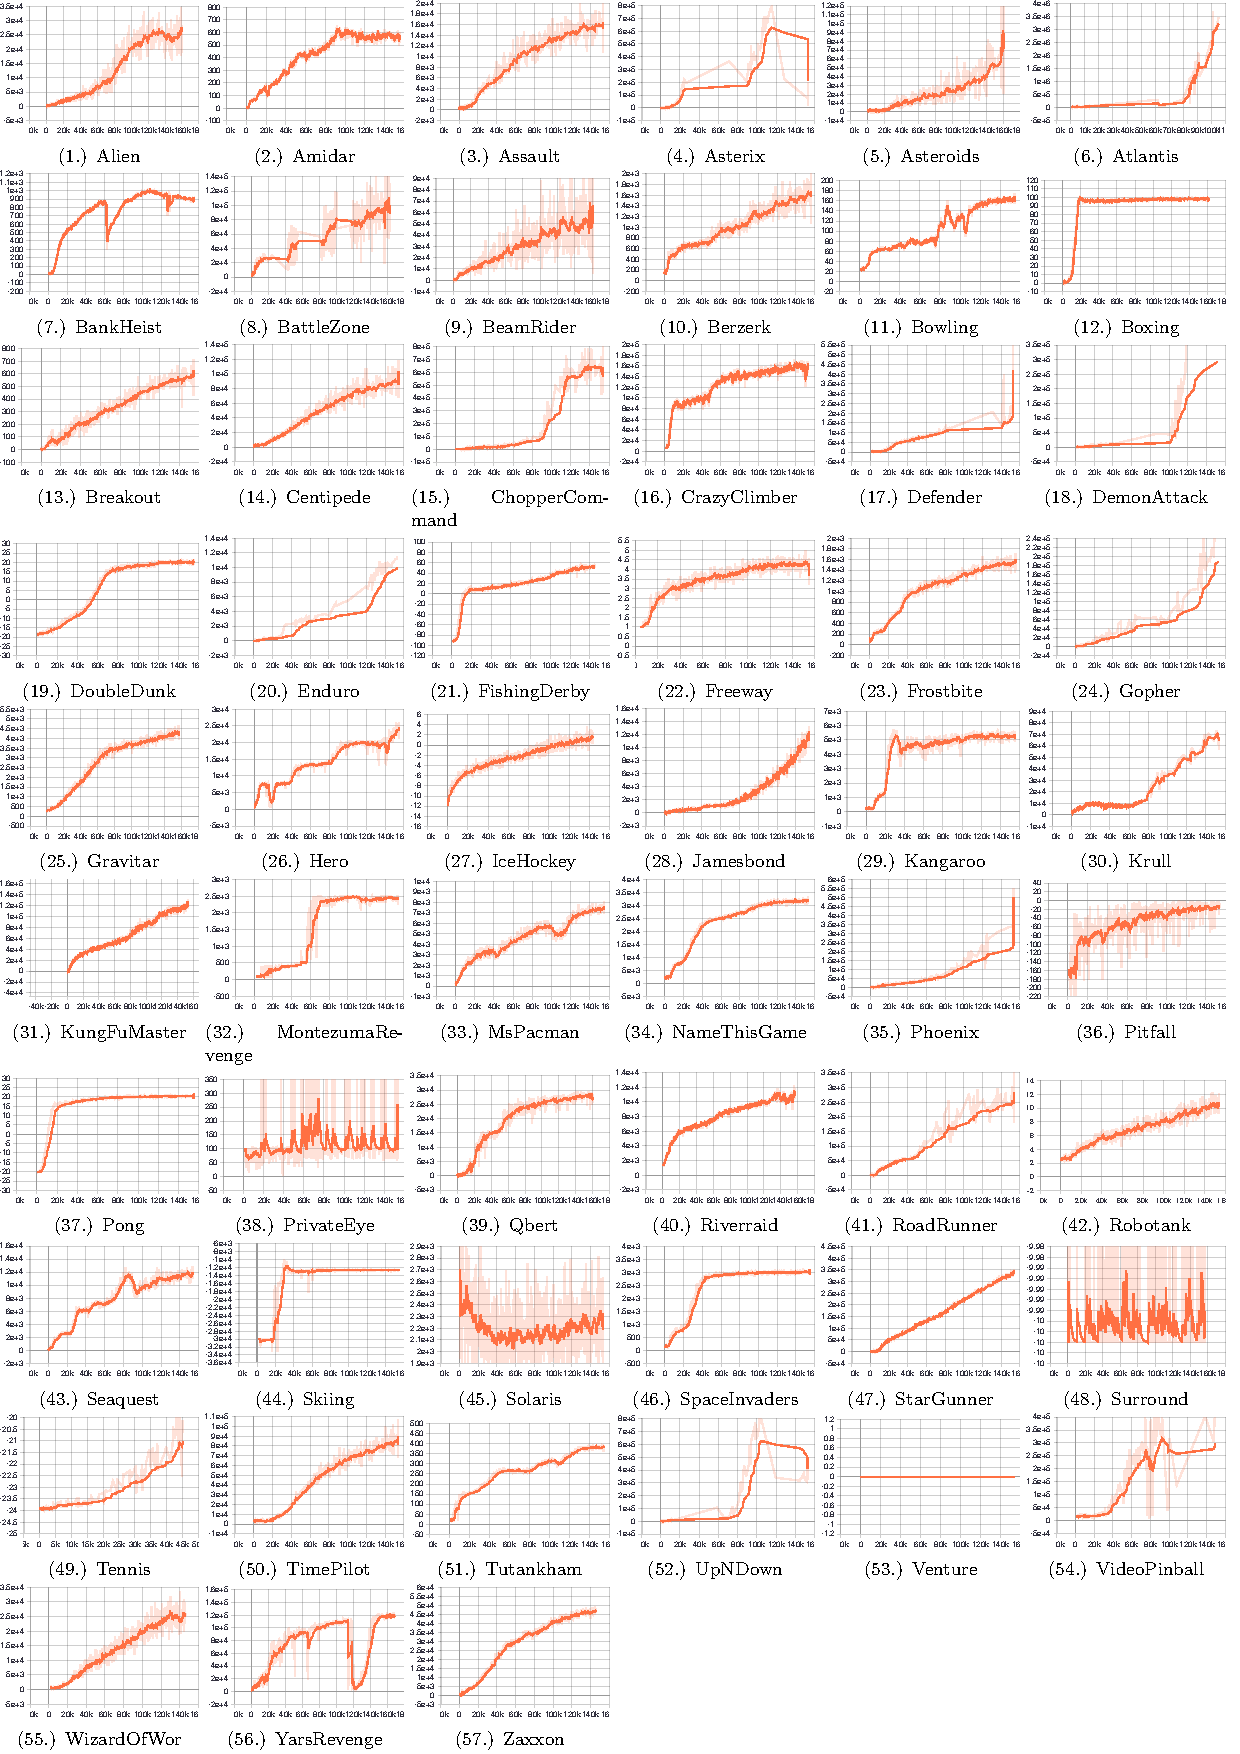
\includegraphics[width=1.0\linewidth]{body/all_fig3.pdf}
\end{figure*}

\clearpage


\end{document}